\section{Results} \label{sec:results}
Several simulations were run with \gls{sispo} in order to assess the capabilities and quality of the output of the three stages, i.e. rendering, compression and reconstruction. Furthermore, the effects of compression using the \gls{jp2} standard on the quality of \gls{3d} model reconstruction were investigated. Table~\ref{tab:sim_params} shows a summary of the simulated scenarios.

\begin{table}[htb]
    \centering
    \caption{Simulation parameters used for investigating capabilities of \gls{sispo}. For each scenario \gls{png}, \gls{jp2} quality 1000, quality 100, quality 10 and quality 1 compression methods were used to investigate the effects of compression.}
    \label{tab:sim_params}
    \begin{tabular}{l|lll}
        \textbf{\gls{sssb} Size [\SI{}{\kilo\meter}]}& \textbf{Encounter Distance [\SI{}{\kilo\meter}]} & \textbf{Number of Images [-]} \\ \hline
        1  & 50  & 120\\
        1  & 100 & 120\\
        1  & 200 & 120\\
        1  & 400 & 120\\
        10 & 50  & 120\\
        10 & 100 & 120\\
        10 & 200 & 120\\
        10 & 400 & 120\\
    \end{tabular}
\end{table}

Two computers were used to create the results. A laptop with \SI{8}{\giga\byte} \gls{ram}, an Intel\textsuperscript{\textregistered}~Core\texttrademark~i7-6700HQ with \SI{4}{} cores at \SI{2.6}{\giga\hertz} and Windows 10. The second is a workstation computer with \SI{16}{\giga\byte} of \gls{ram}, an Intel\textsuperscript{\textregistered}~Core\texttrademark~i7-8700 processor with \SI{6}{} cores at \SI{3.2}{\giga\hertz} and Ubuntu 18.04.3 LTS. During simulation, it was noticed that the reconstruction pipeline is more often successful when using the laptop running Windows. Therefore, images were rendered on the Linux computer and reconstructions were made using the Windows computer.

\subsection{Rendering} \label{sec:results_sim}
A subset of all settings was kept constant for all simulations. The instrument settings are presented in Table~\ref{tab:inst_settings} and the settings for the \gls{sssb} in Table~\ref{tab:sssb_settings}. The specific values were chosen in order to mimic the scenario in~\cite{Pajusalu2019CharacterizationMapping}.

\begin{table}[htb]
    \centering
    \caption{Instrument settings used in all simulation scenarios presented in Table~\ref{tab:sim_params}. The parameters represent the preliminary instrument design presented in~\cite{Pajusalu2019CharacterizationMapping}.}
    \label{tab:inst_settings}
    \begin{tabular}{l|l}
        \textbf{Parameter Name} & \textbf{Value} \\ \hline
        res       & $\SI{2464}{} \times \SI{2054}{}$   \\
        pix\_l        & \SI{3.45}{\micro\meter}     \\
        focal\_l       & \SI{230}{\milli\meter}     \\
        aperture\_d     &  \SI{4}{\centi\meter} \\
        wavelength  & \SI{550}{\nano\meter} \\
        quantum\_eff & \SI{0.25}{} \\
        color\_depth & \SI{8}{\bit}
    \end{tabular}
\end{table}

\begin{table}[htb]
    \centering
    \caption{\gls{sssb} trajectory settings used in all simulation scenarios presented in Table~\ref{tab:sim_params}. The orbital elements and rotation rate of Didymos were used, comparable to~\cite{Pajusalu2019CharacterizationMapping}.}
    \label{tab:sssb_settings}
    \begin{tabular}{l|l}
        \textbf{Parameter Name} & \textbf{Value} \\ \hline
        a & \SI{1.644641475071416}{\astronomicalunit}   \\
        e & \SI{3.838774437558215E-01}{}\\
        i & \SI{3.408231185574551E+00}{\radian}\\
        P &  \SI{7.703805051391988E+02}{\radian} \\
        omega  & \SI{3.192958853076784E+02}{\radian} \\
        Omega & \SI{7.320940216397703E+01}{\radian} \\
        M & \SI{1.967164895190036E+02}{\radian} \\
        date & 2017-08-19T00:00:00.000 \\
        rotation\_rate & \SI{8133.48}{\per\second} \\
        albedo & \SI{0.15}{} \\
        max\_dim & \SI{512}{}
    \end{tabular}
\end{table}

\begin{table}[htb]
    \centering
    \caption{Propagation and rendering settings used in all simulation scenarios presented in Table~\ref{tab:sim_params}.}
    \label{tab:sim_settings}
    \begin{tabular}{l|l}
        \textbf{Parameter Name} & \textbf{Value} \\ \hline
        duration       & \SI{120}{\second}   \\
        encounter\_date & 2017-08-15T12:00:00.000\\
        frames       & \SI{120}{}     \\
        relative\_velocity     &  \SI{10}{\kilo\meter\per\second} \\
        with\_terminator  & \SI{0}{} \\
        with\_sunnyside & \SI{1}{} \\
        timesampler\_mode & \SI{1}{} \\
        exposure & \SI{0}{} \\
        samples & \SI{48}{} \\
        device & \gls{gpu} \\
        tile\_size & \SI{512}{} \\
        with\_clipping & \SI{1}{}
    \end{tabular}
\end{table}

\subsubsection{Image Comparison}
In a first step, the overall image quality is compared visually to real images. A set of images at different distances of nuclei with different sizes is depicted in Figure~\ref{fig:render_quali_comparison}. A set of five images from asteroid Bennu taken by the PolyCam aboard the \textit{OSIRIS-REx} mission is shown in Figure~\ref{fig:render_quali_bennu}. Additionally, the rendered images are compared to images of comet \gls{67p} taken by the OSIRIS imager aboard the \textit{Rosetta} spacecraft. Figure~\ref{fig:render_quali_67p} shows one image that represents all important features of \gls{67p}. A collection of several views of the comet \gls{81p}, also known as Wild 2, are shown in Figure~\ref{fig:render_quali_81p}. \Gls{81p} was visited during the \textit{Stardust} mission~\cite{Brownlee2003Stardust:Mission}.

\begin{figure}[htb]
    \centering
    \begin{subfigure}[b]{0.48\textwidth}
        \centering
        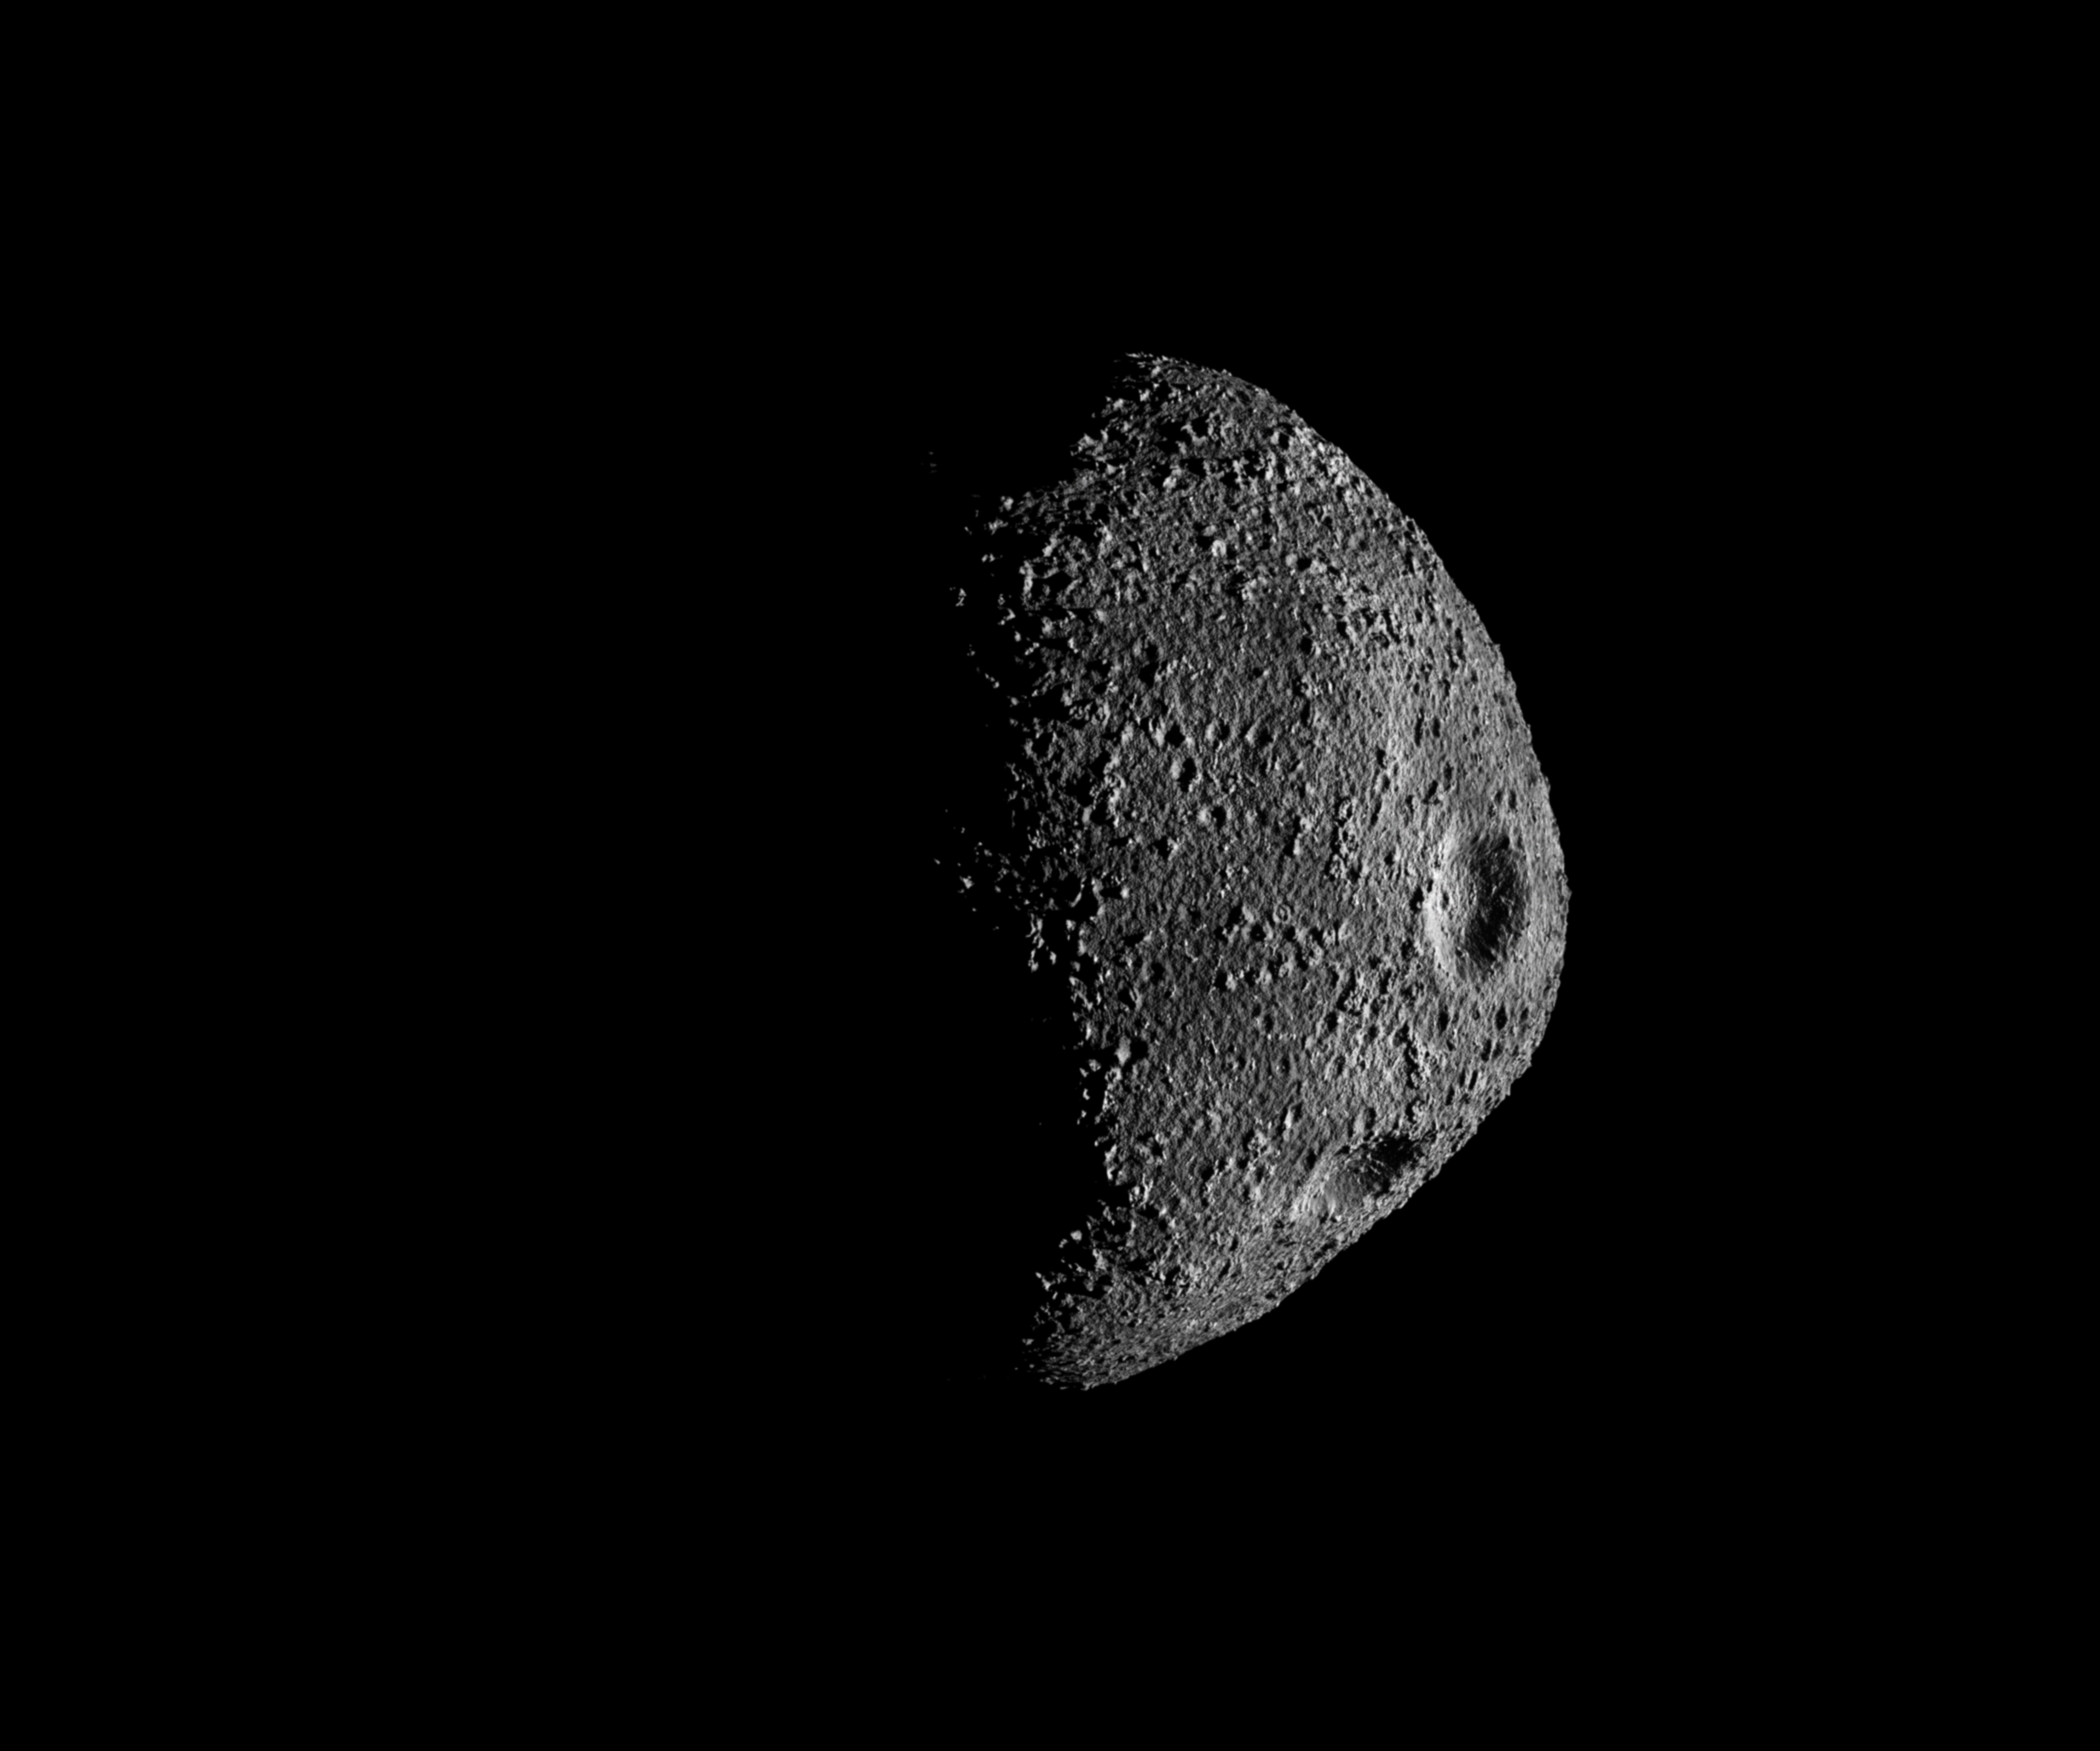
\includegraphics[width=\textwidth]{doc/thesis/0_figures/procedural_terrain/50_10_Inst_2017-08-15T115755-845000.png}
        \caption{}
        \label{fig:render_quali_comparison_1}
    \end{subfigure}
    \begin{subfigure}[b]{0.48\textwidth}
        \centering
        \includegraphics[width=\textwidth]{doc/thesis/0_figures/procedural_terrain/50_10_Inst_2017-08-15T115855-260000.png}
        \caption{}
        \label{fig:render_quali_comparison_2}
    \end{subfigure}
    \\
    \begin{subfigure}[b]{0.48\textwidth}
        \centering
        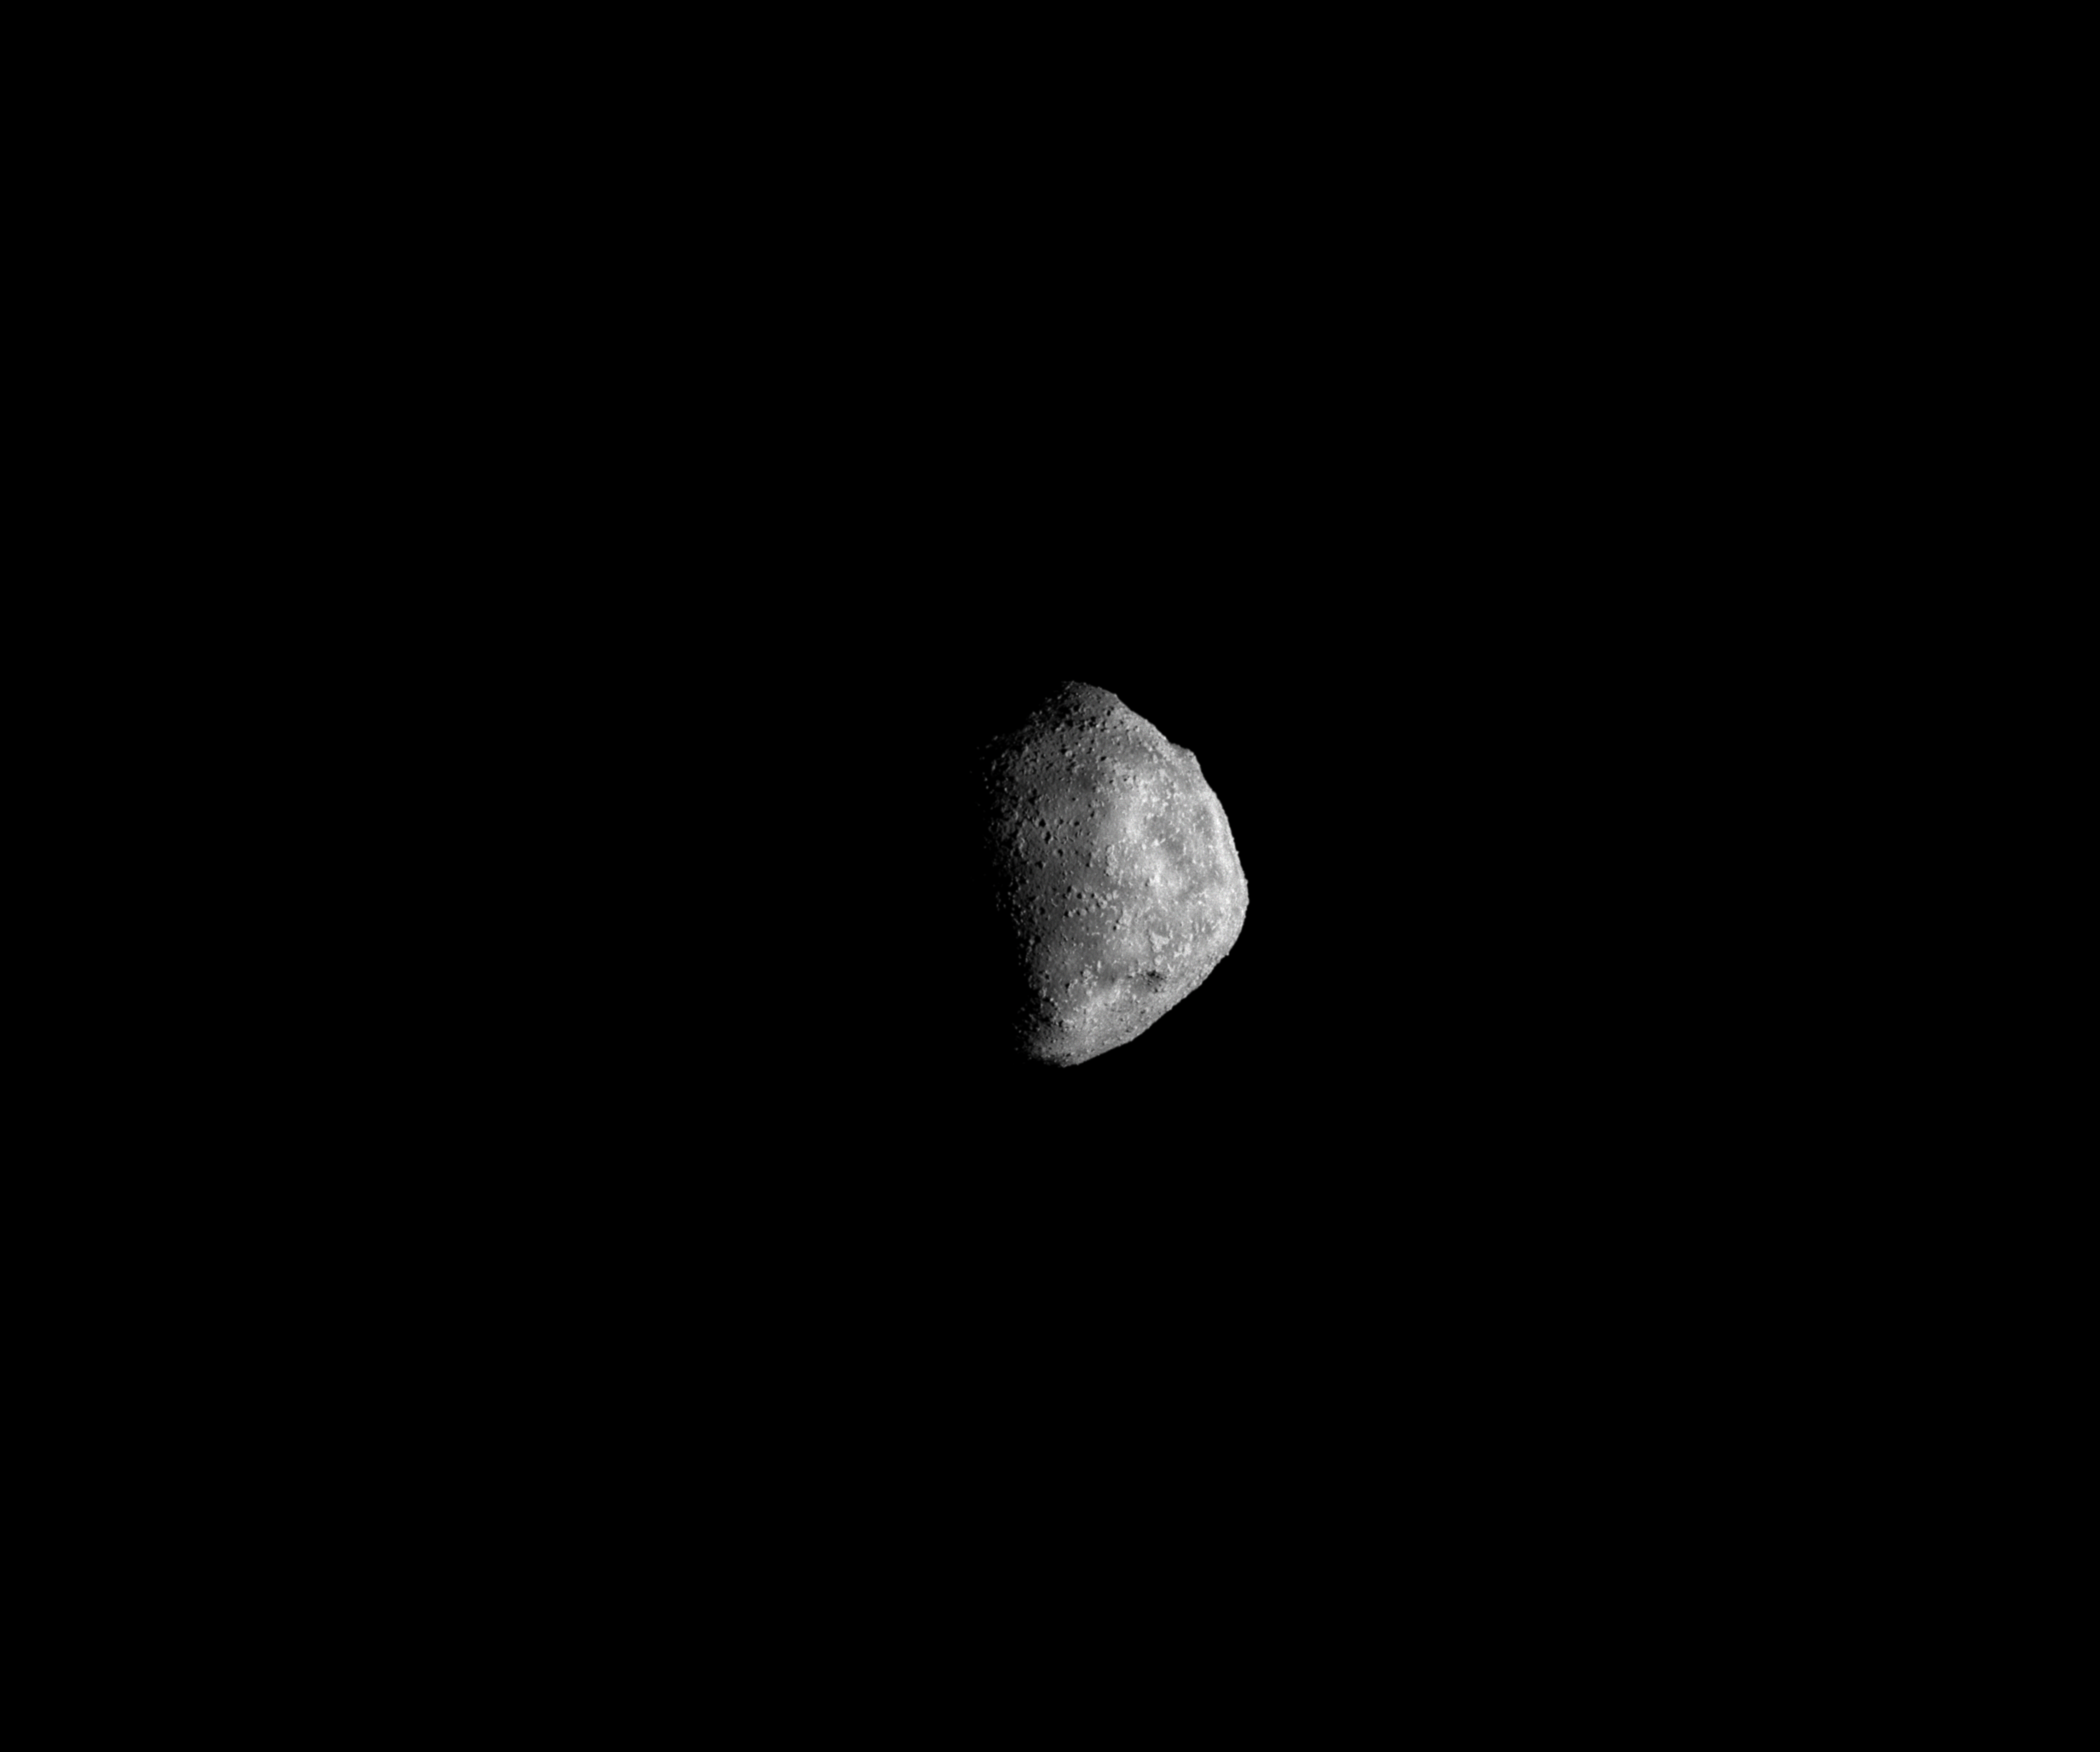
\includegraphics[width=\textwidth]{doc/thesis/0_figures/procedural_terrain/50_1_Inst_2017-08-15T115837-133000.png}
        \caption{}
        \label{fig:render_quali_comparison_3}
    \end{subfigure}
    \begin{subfigure}[b]{0.48\textwidth}
        \centering
        \includegraphics[width=\textwidth]{doc/thesis/0_figures/procedural_terrain/50_1_Inst_2017-08-15T115851-232000.png}
        \caption{}
        \label{fig:render_quali_comparison_4}
    \end{subfigure}
    \caption{Rendered images of an \gls{sssb} nucleus of different sizes from varying distances. (a) Nucleus of \SI{10}{\kilo\meter} from \SI{566}{\kilo\meter} distance. (b) Nucleus of \SI{10}{\kilo\meter} from \SI{106}{\kilo\meter} distance. (c) Nucleus of \SI{1}{\kilo\meter} from \SI{149}{\kilo\meter} distance. (d) Nucleus of \SI{1}{\kilo\meter} from \SI{50}{\kilo\meter} distance.}
    \label{fig:render_quali_comparison}
\end{figure}

\begin{figure}[htb]
    \centering
    \begin{subfigure}[b]{0.59\textwidth}
        \centering
        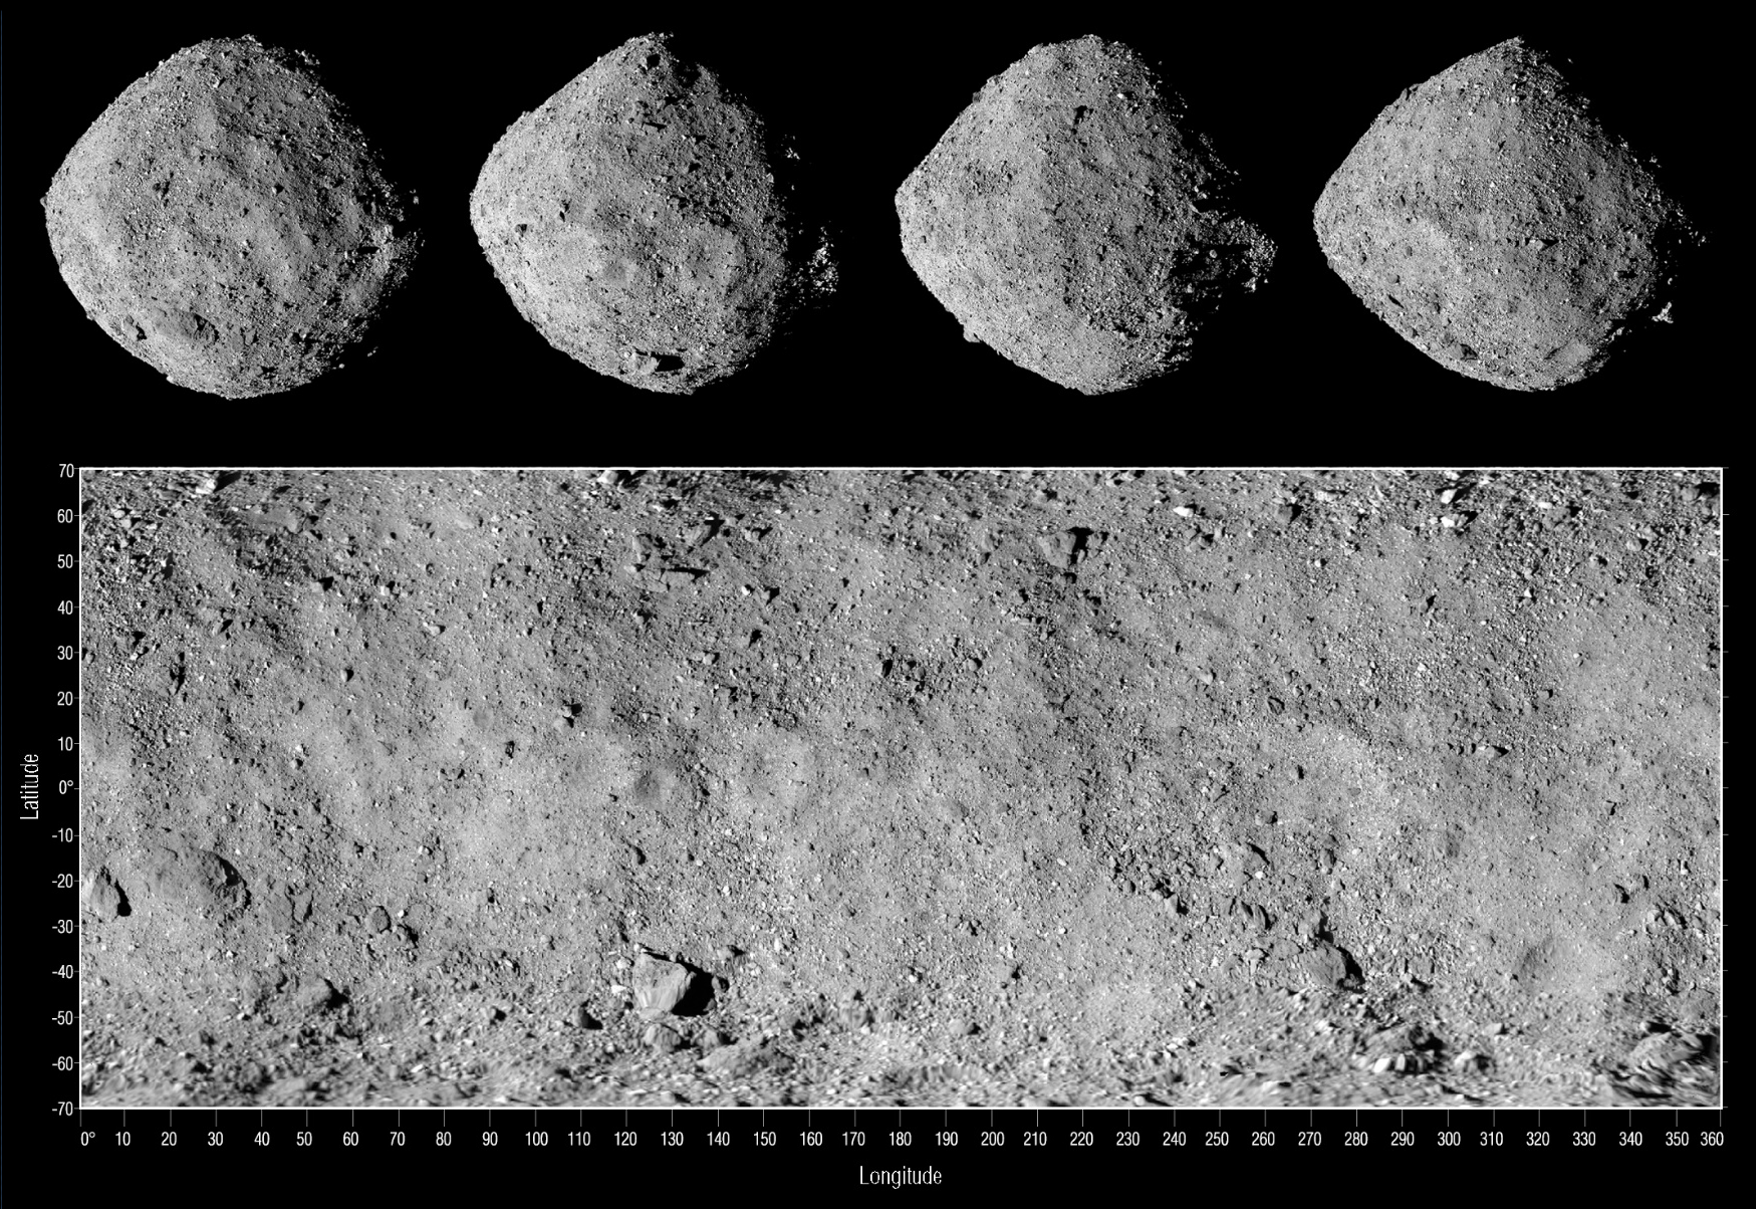
\includegraphics[width=\textwidth]{doc/thesis/0_figures/procedural_terrain/2963_Bennu.png}
        \caption{}
        \label{fig:render_quali_bennu}
    \end{subfigure} %
    \begin{subfigure}[b]{0.4\textwidth}
        \centering
        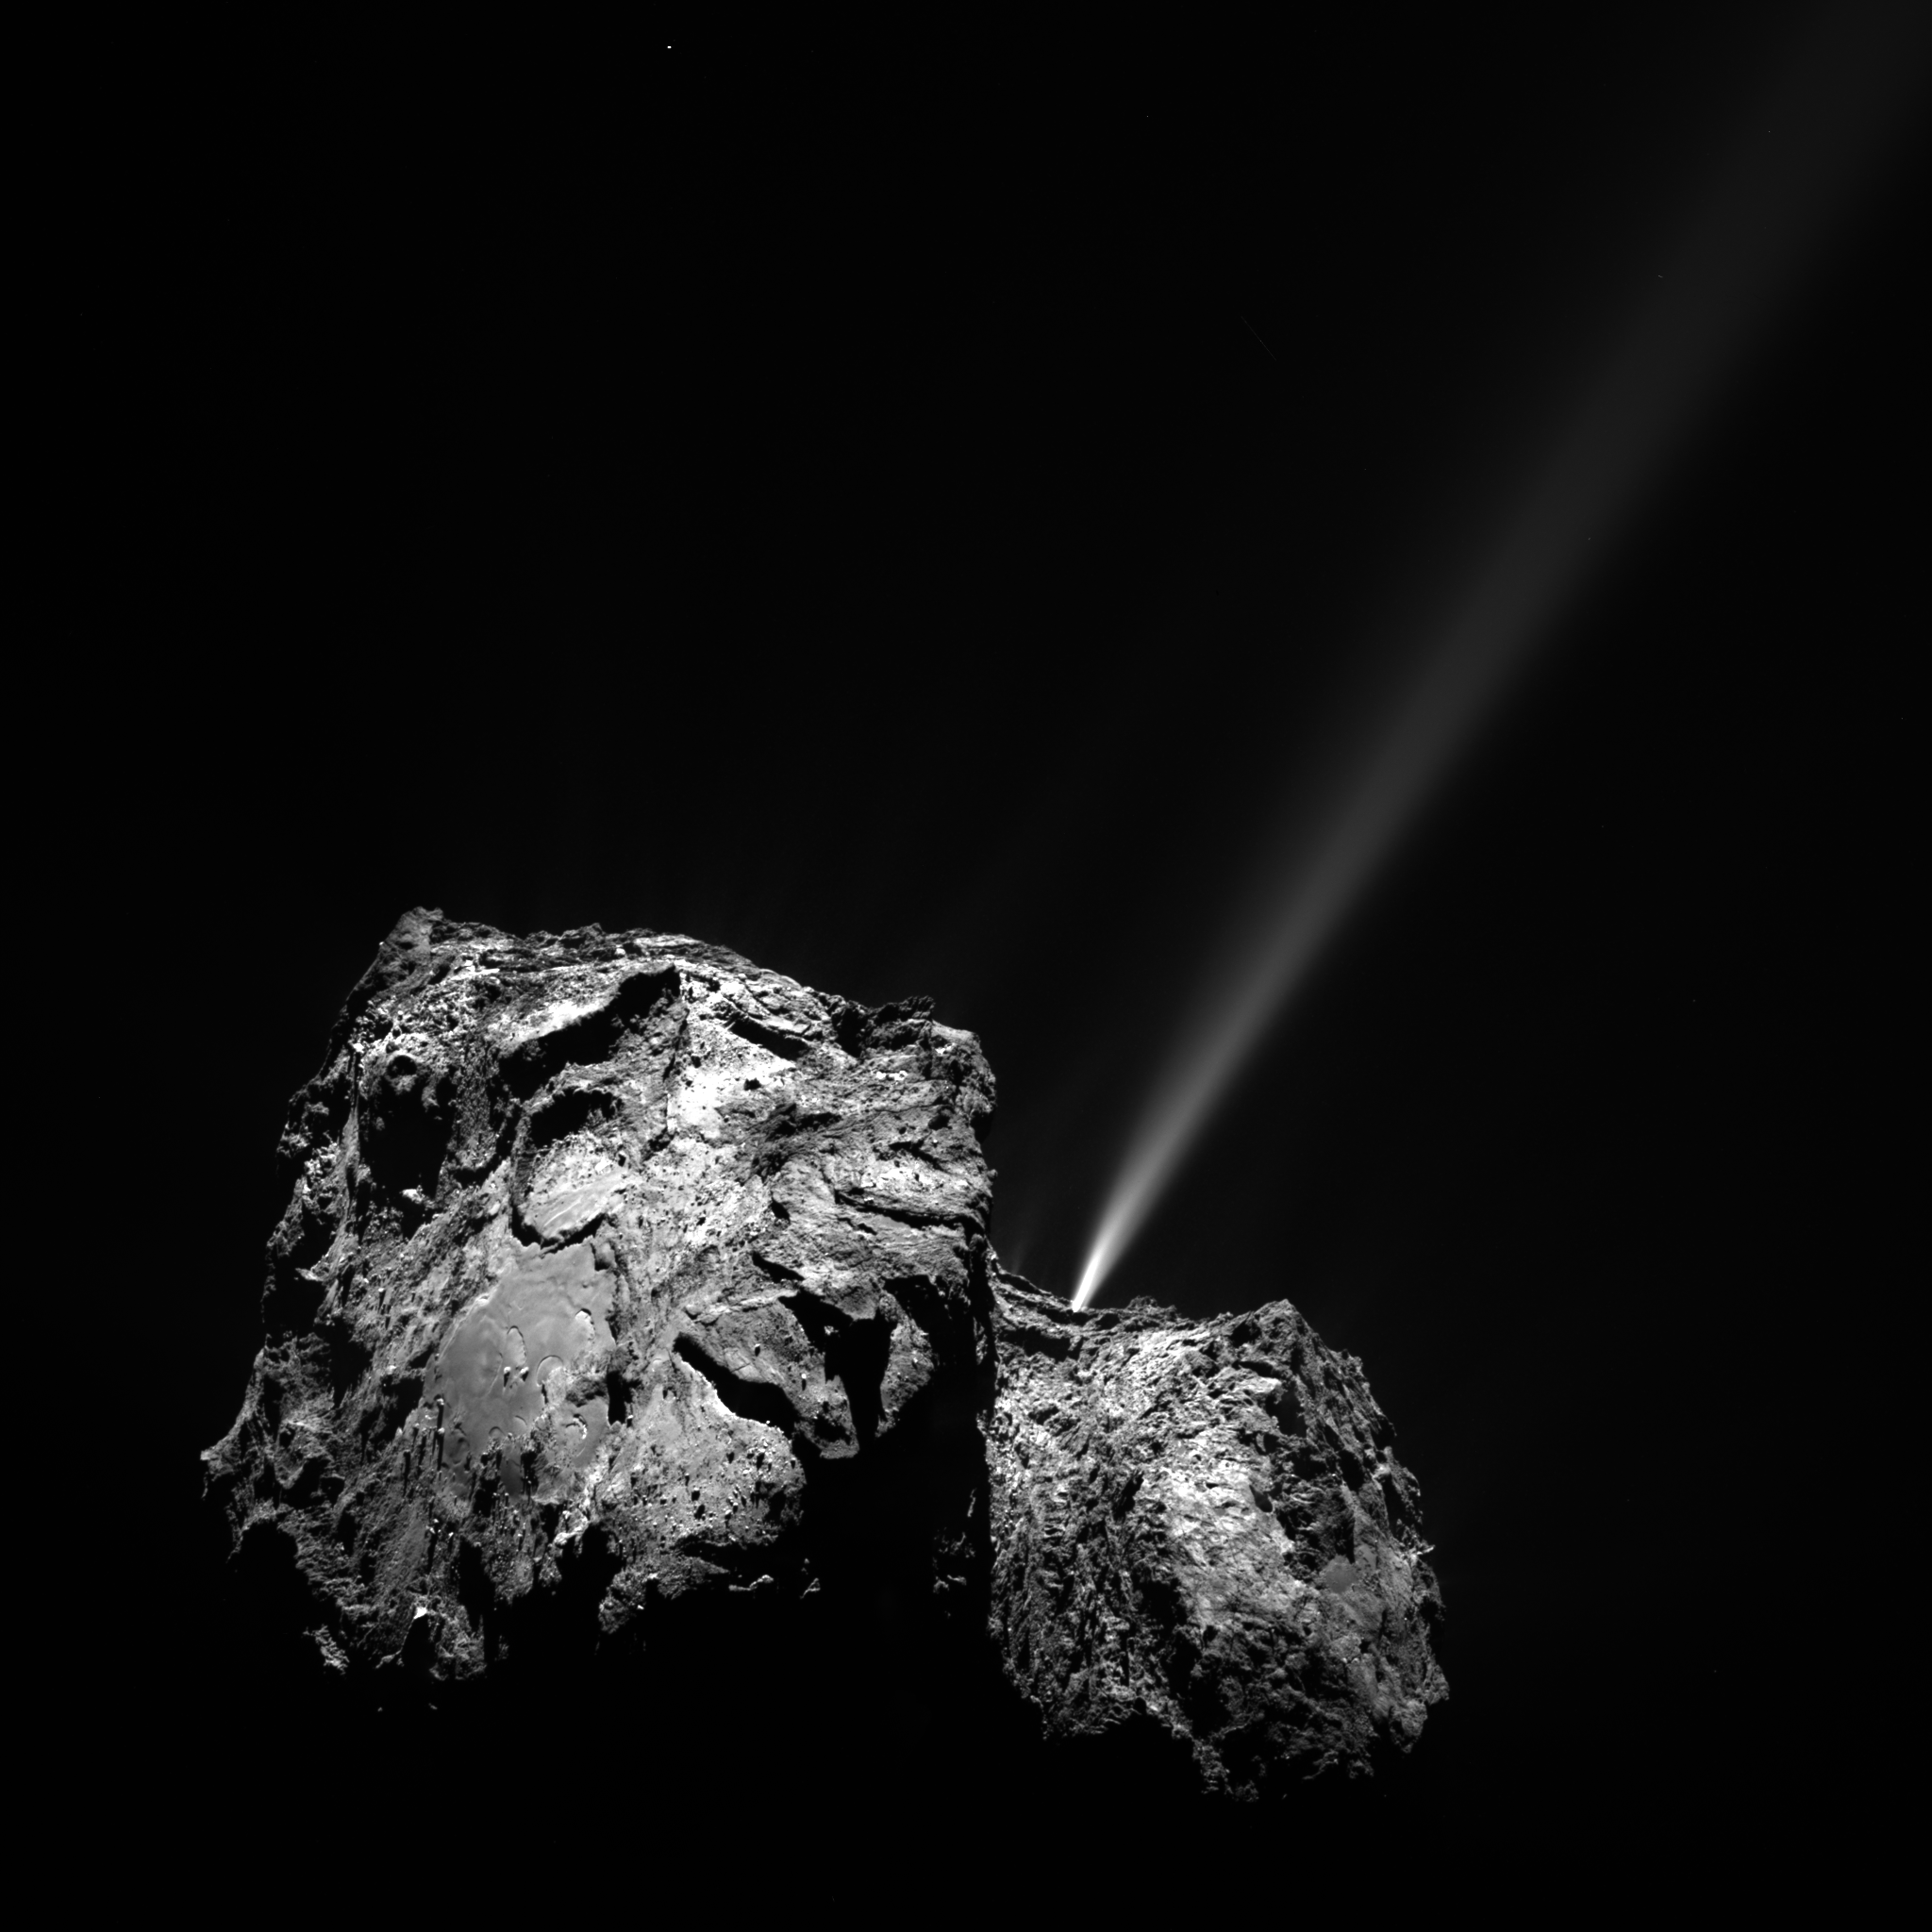
\includegraphics[width=\textwidth]{doc/thesis/0_figures/procedural_terrain/67P_CG.PNG}
        \caption{}
        \label{fig:render_quali_67p}
    \end{subfigure}
    \\
    \begin{subfigure}[b]{0.6\textwidth}
        \centering
        \includegraphics[width=\textwidth]{doc/thesis/0_figures/procedural_terrain/Wild2.jpg}
        \caption{}
        \label{fig:render_quali_81p}
    \end{subfigure}
    \label{fig:render_quali}
    \caption{(a) Four images of asteroid Bennu and a global surface mosaic. These images were taken by the PolyCam aboard the \textit{OSIRIS-REx} mission~\cite{NASAFourBennu}. (b) Representative image of comet \acrlong{67p}. The image was taken by the OSIRIS imager aboard the \textit{Rosetta} mission~\cite{OSIRISArchiveb}. (c) Collection of images of comet \acrlong{81p} taken during the \textit{Stardust} mission by its navigation camera~\cite{StardustImages}.}
\end{figure}

While all images show pits, the overall appearance of the rendered images resembles the smoother pits of Bennu better than the sharper pits of \gls{67p} or \gls{81p}. The overall looks of the rendered images resemble the real images of Bennu well. The rocks and boulders present on Bennu's surface appear similar to the rocks and boulders in the rendered images. When comparing the rendered images to the images of \gls{67p} or \gls{81p}, the most pronounced difference are the jets. \Gls{sispo} does not yet contain a gas and dust model that would produce a coma or jets and therefore these are missing in the rendered images. While the surface of both comets feature some rocks and boulders, there surfaces more defined by ridge-like structures. This type of feature is missing in the rendered images. Hence, the rendering output of \gls{sispo} better represents asteroids than comets.

Through procedural terrain generation, \gls{sispo} produces results for a large range of encounter distances. Example images with different surface distances and \gls{sssb} sizes are shown in Figure~\ref{fig:render_quali_comparison}.It is visible from Figure~\ref{fig:render_quali_comparison} that surface features and details do not degrade visually. Moving closer to the surface reveals more details, such as tiny bumps between larger structures which are not visible from larger distances. The visible quality of surface features is defined by the shader implementation. 

\subsubsection{Image Composition}
The composition process uses raw images rendered with Blender and produces photometrically calibrated images. An example set of four images consisting of two images before and after calibration is shown in Figure~\ref{fig:composition_before_after}. All four images were converted to \SI{8}{\bit} images. Two effects can be seen. First, the original images differ in there overall brightness. This difference is removed by the calibration. Secondly, images become brighter by the calibration process. 

\begin{figure}[htb]
    \centering
    \begin{subfigure}[b]{0.48\textwidth}
        \centering
        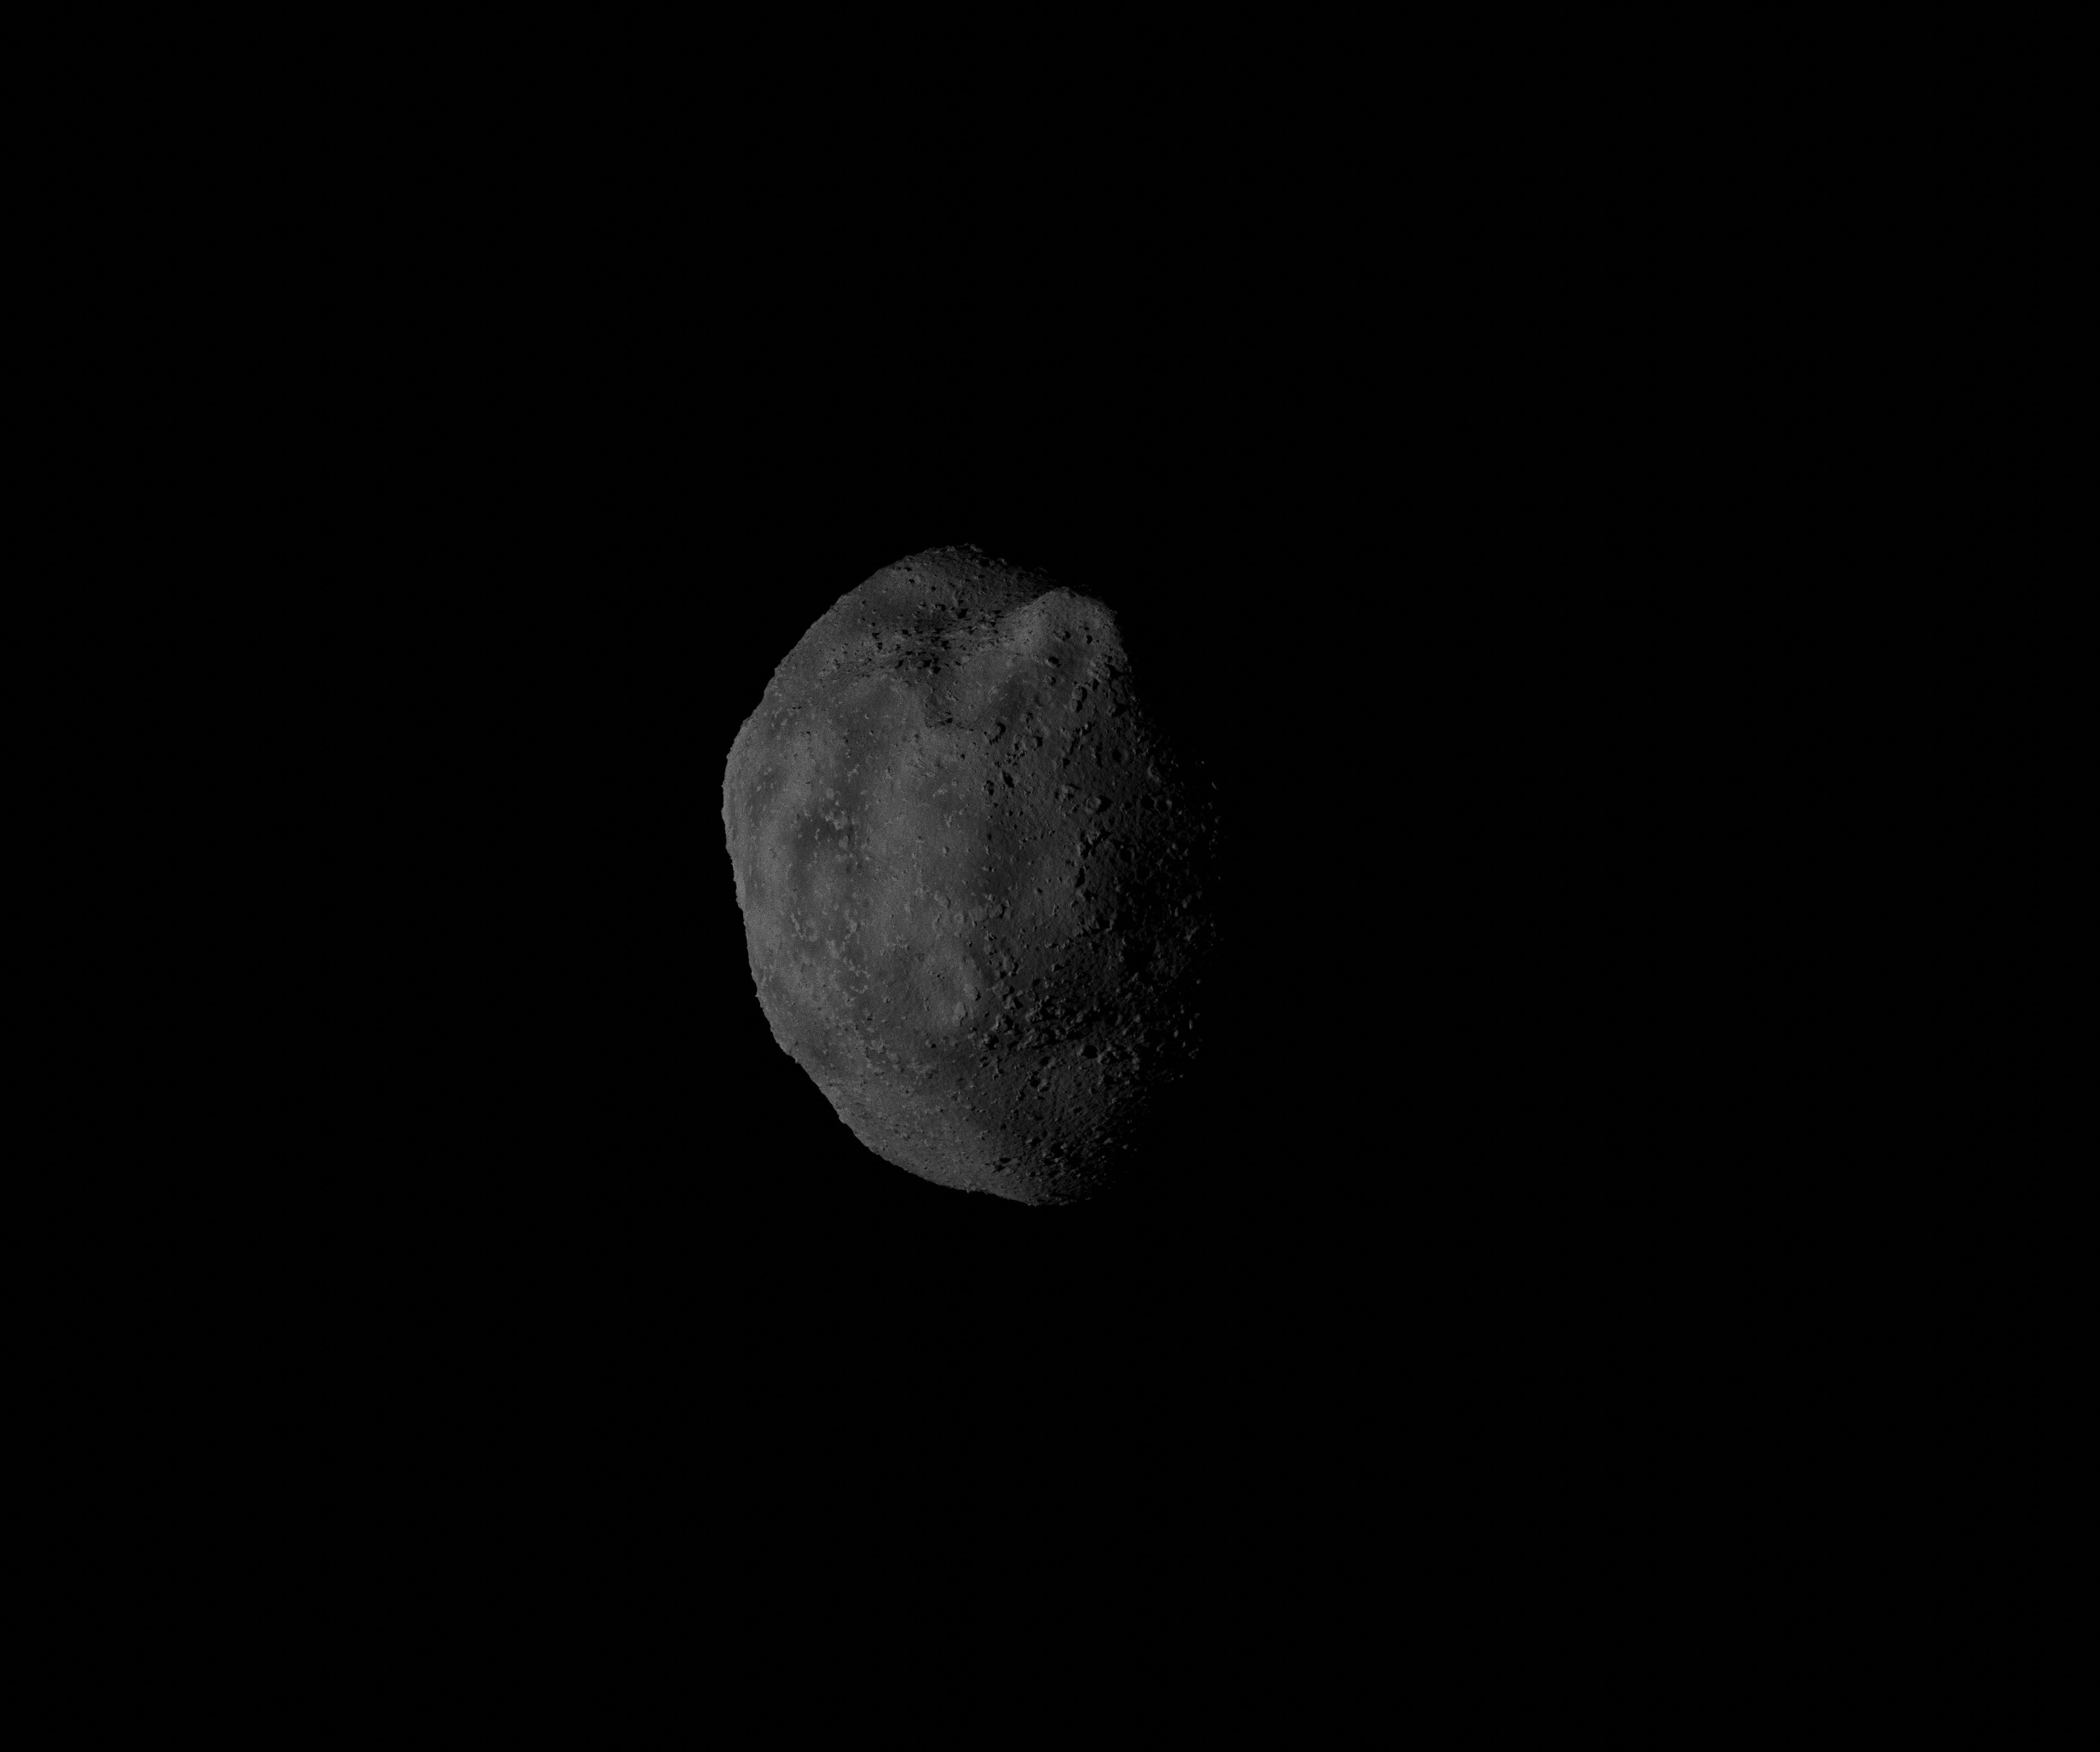
\includegraphics[width=\textwidth]{doc/thesis/0_figures/rendering_lighting/SssbOnly_2017-08-15T115858-281000.jpg}
        \caption{}
        \label{fig:composition_before_1}
    \end{subfigure}
    \begin{subfigure}[b]{0.48\textwidth}
        \centering
        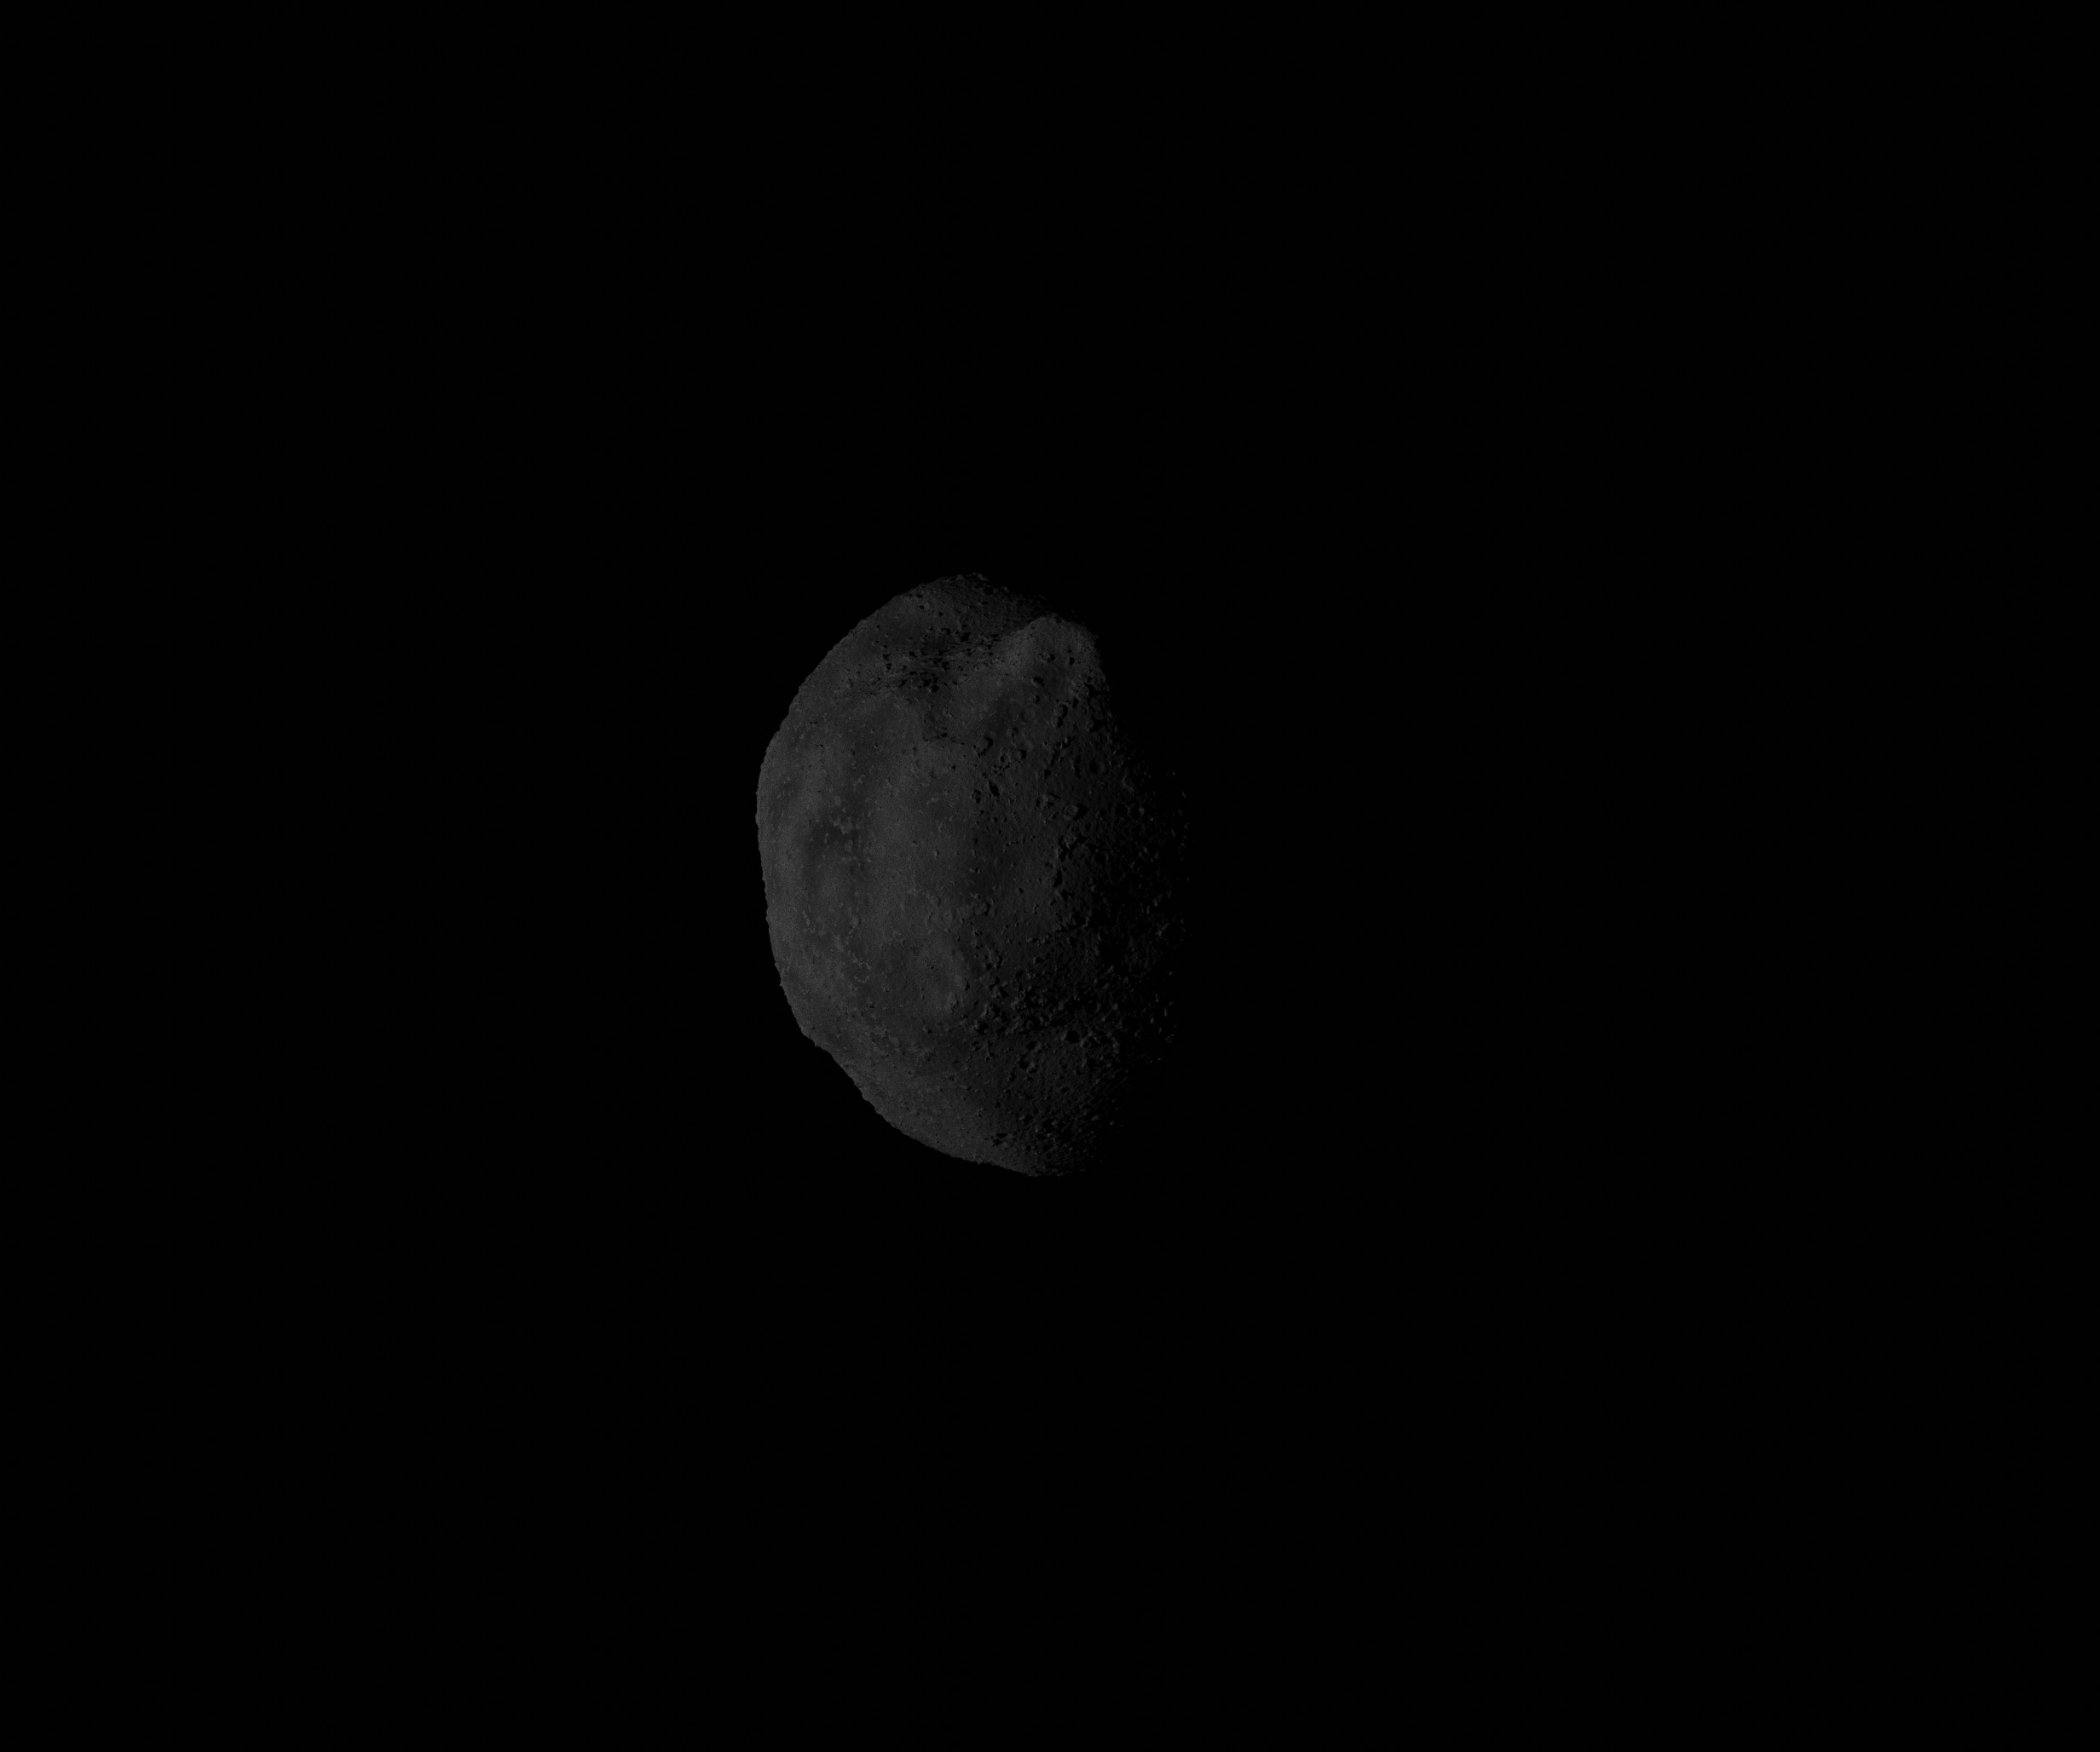
\includegraphics[width=\textwidth]{doc/thesis/0_figures/rendering_lighting/SssbOnly_2017-08-15T115859-288000.jpg}
        \caption{}
        \label{fig:composition_before_2}
    \end{subfigure}
    \\
    \begin{subfigure}[b]{0.48\textwidth}
        \centering
        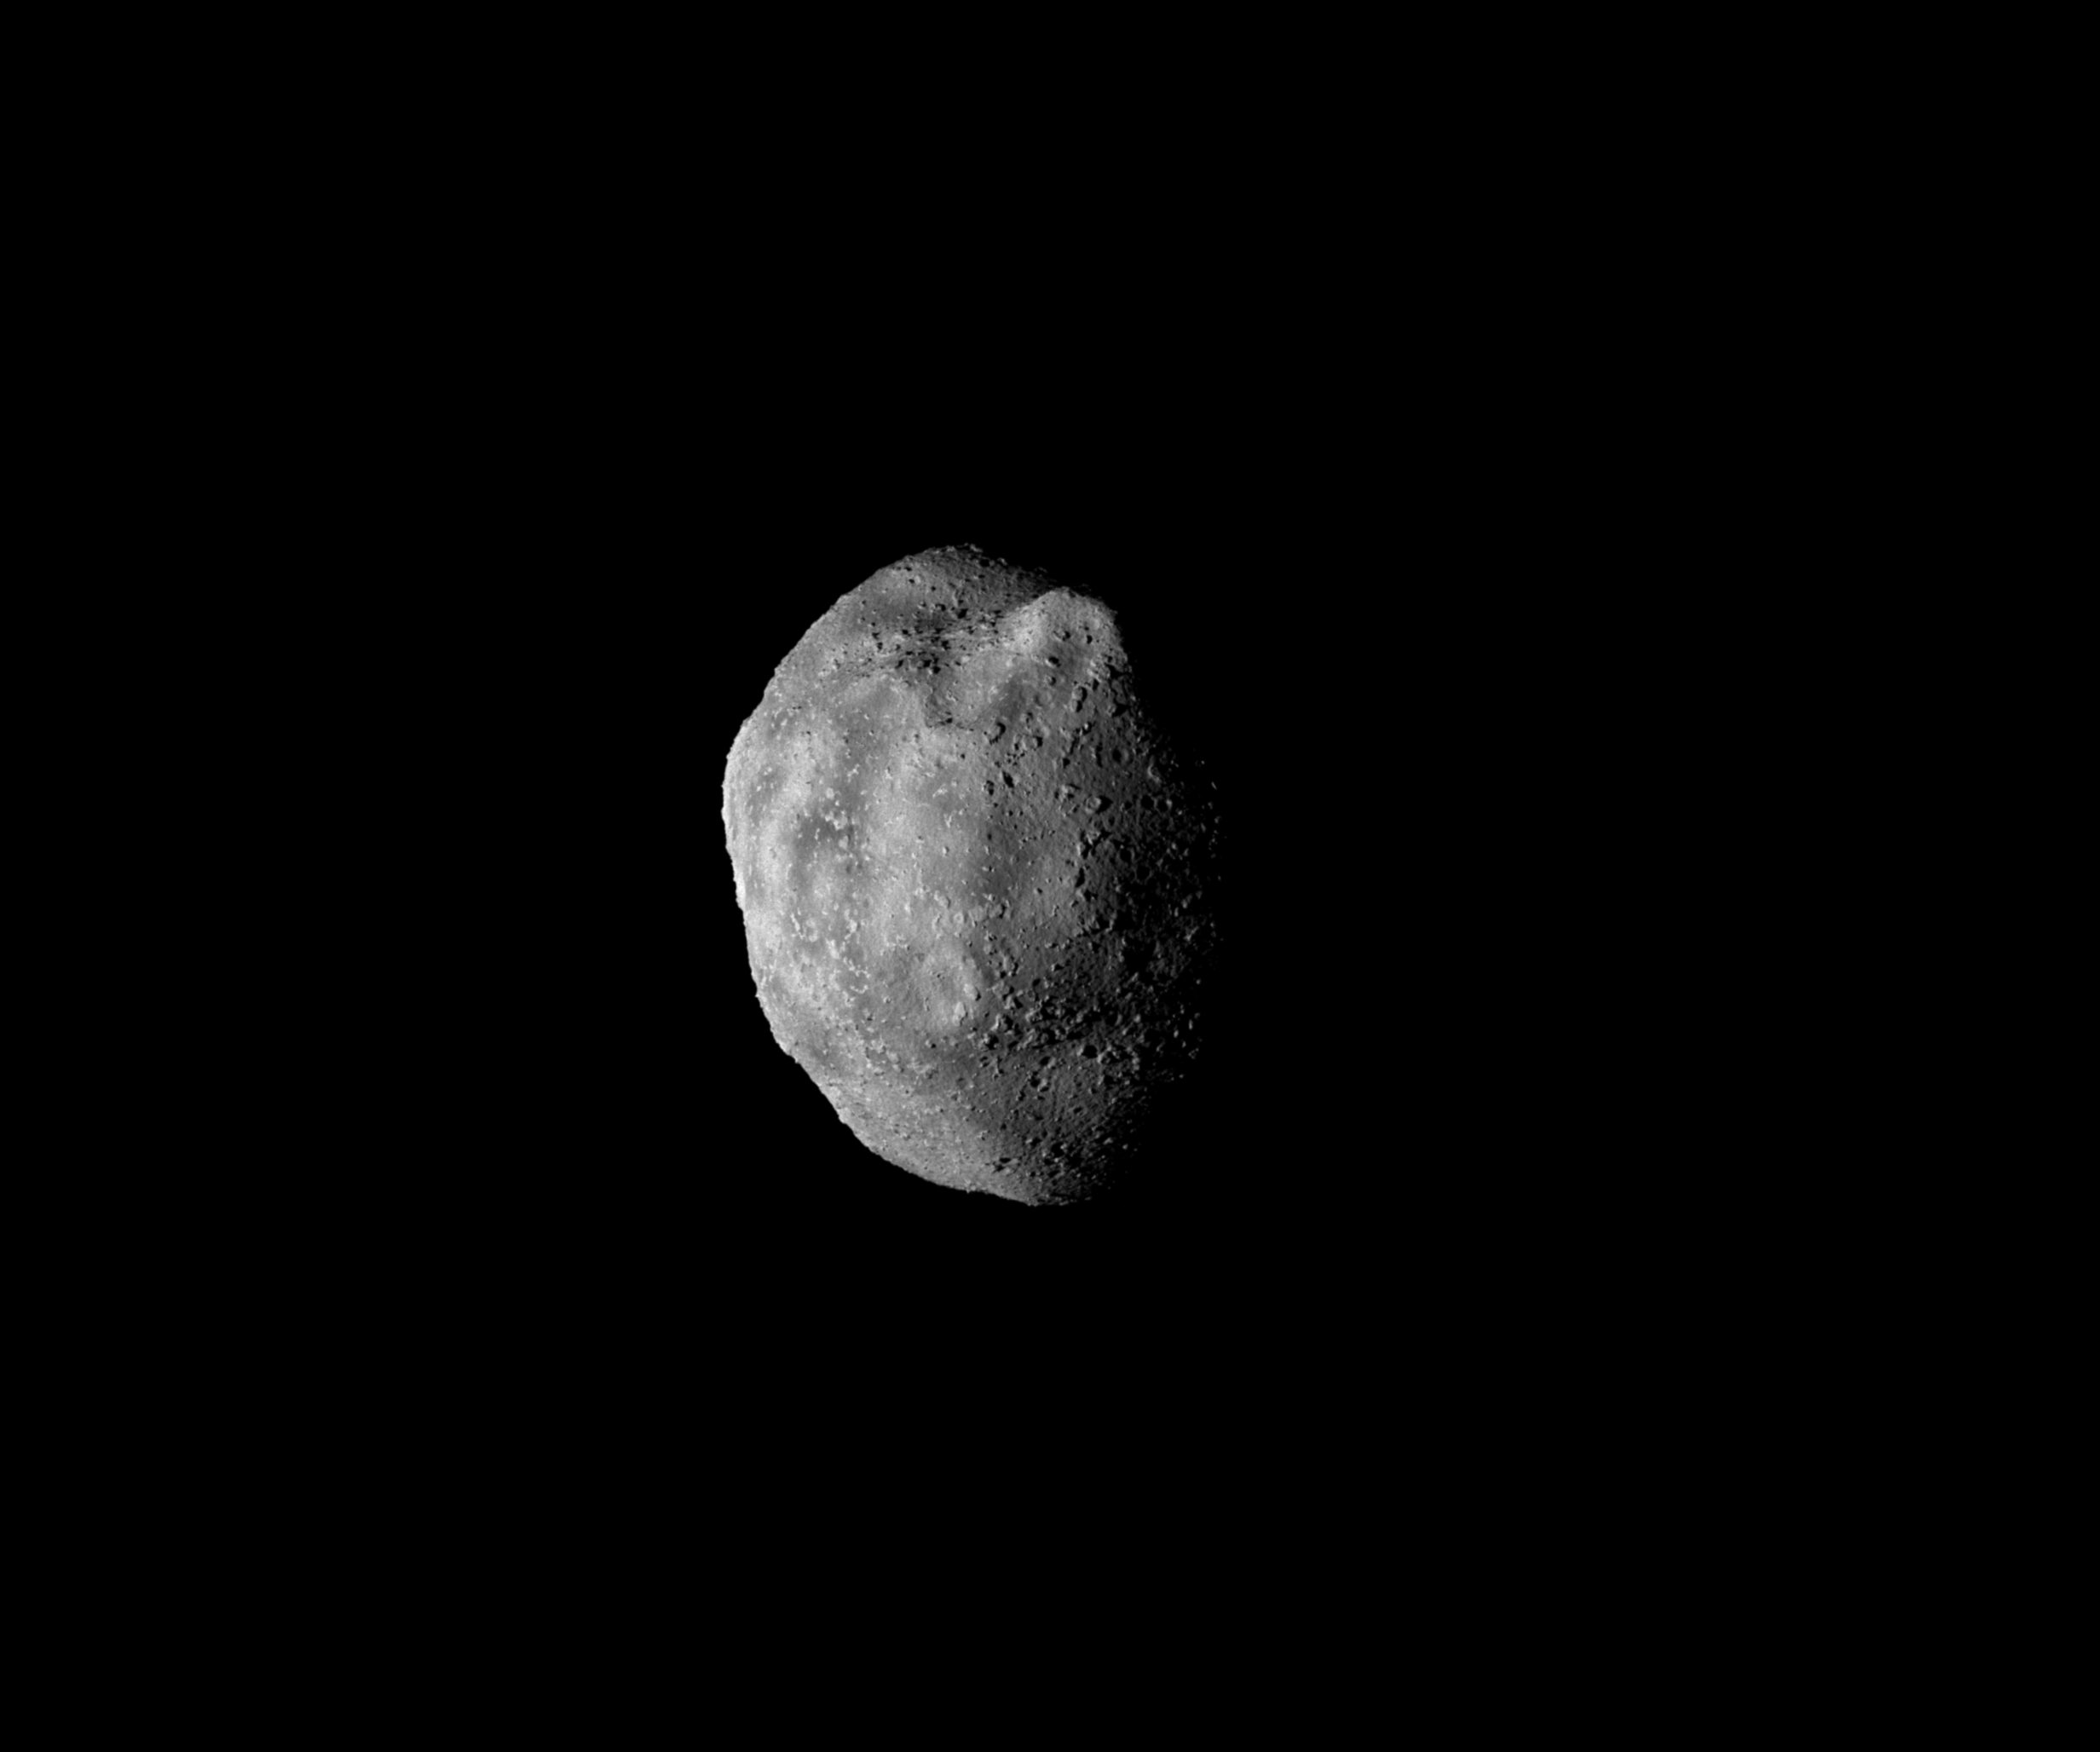
\includegraphics[width=\textwidth]{doc/thesis/0_figures/rendering_lighting/Inst_2017-08-15T115858-281000.png}
        \caption{}
        \label{fig:composition_after_1}
    \end{subfigure}
    \begin{subfigure}[b]{0.48\textwidth}
        \centering
        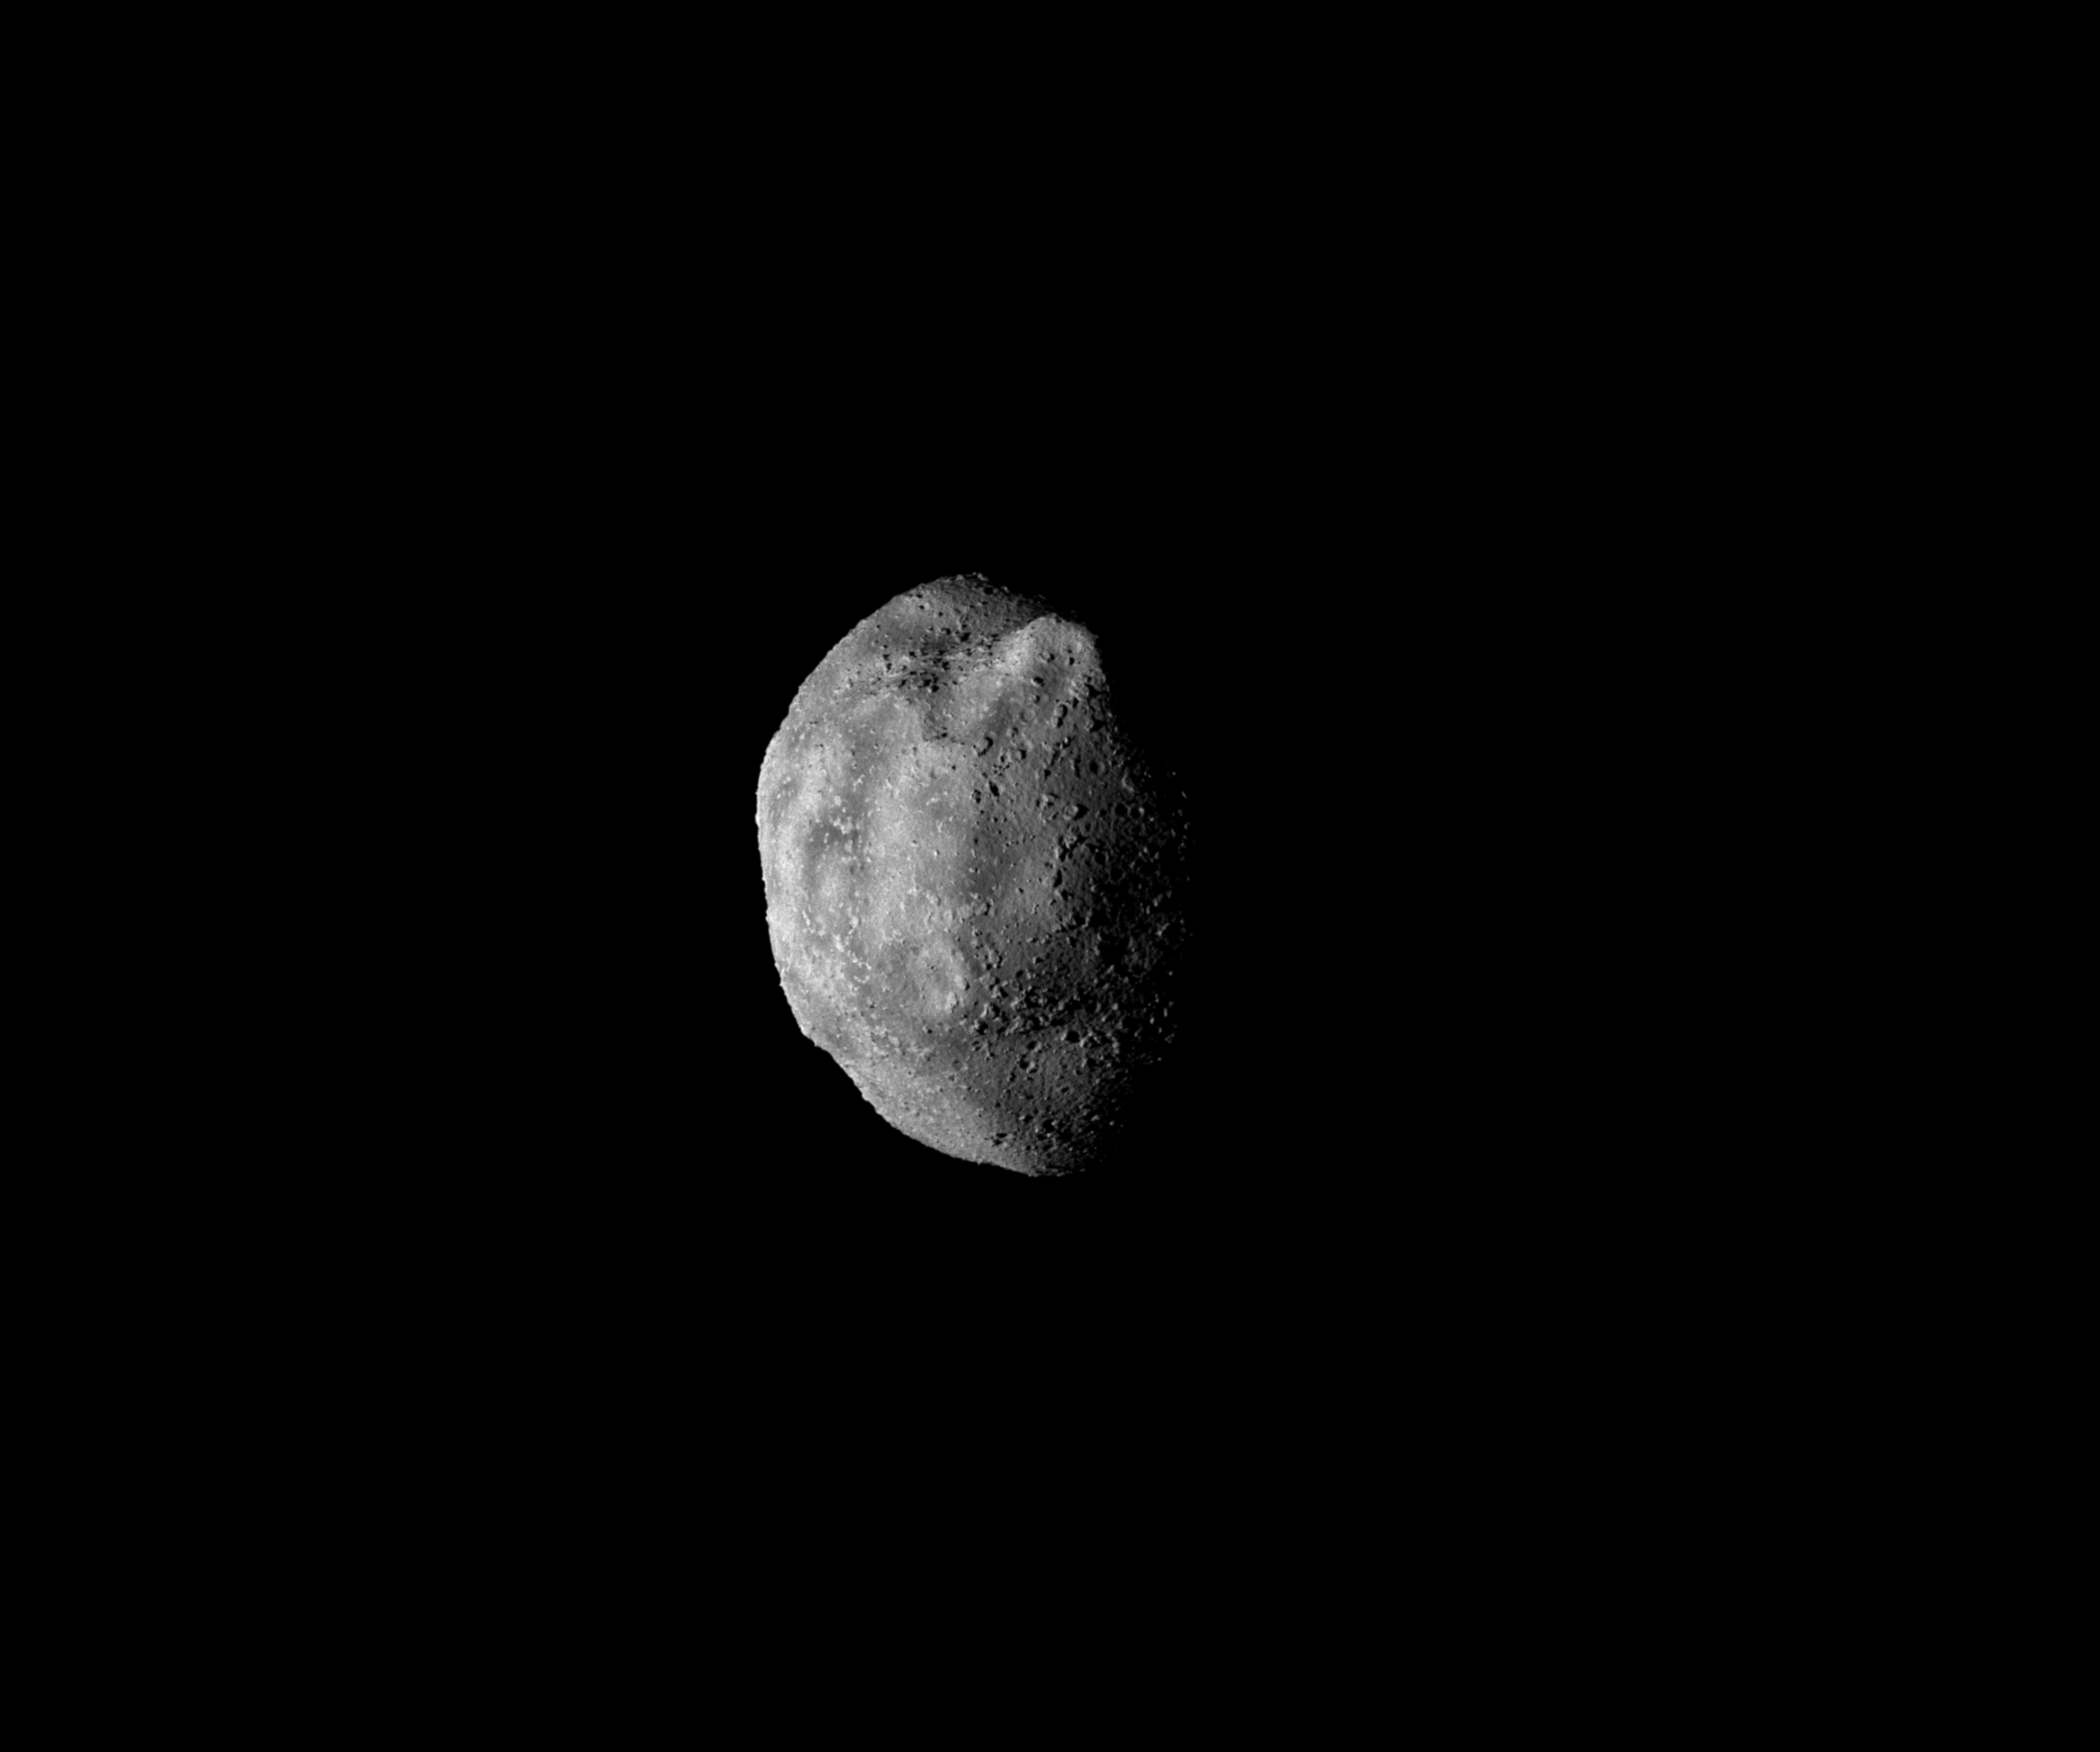
\includegraphics[width=\textwidth]{doc/thesis/0_figures/rendering_lighting/Inst_2017-08-15T115859-288000.png}
        \caption{}
        \label{fig:composition_after_2}
    \end{subfigure}
    \caption{Two consecutive images before and after the composition process. The nucleus is much brighter than background stars thus no stars are visible in these images after calibration. (a)~Image 1 before calibration. (b)~Image 2 before calibration. (c)~Image 1 after calibration. (d)~Image 2 after calibration.}
    \label{fig:composition_before_after}
\end{figure}

% As Figures~\ref{fig:composition_after_1} and \ref{fig:composition_after_2} show, the composition properly calibrates the overall brightness of different images. However, there are sometimes darker and brighter patches within images that are not yet calibrated properly. Figure 

% \begin{figure}[htb]
%     \centering
%         \begin{subfigure}[b]{0.32\textwidth}
%             \centering
%             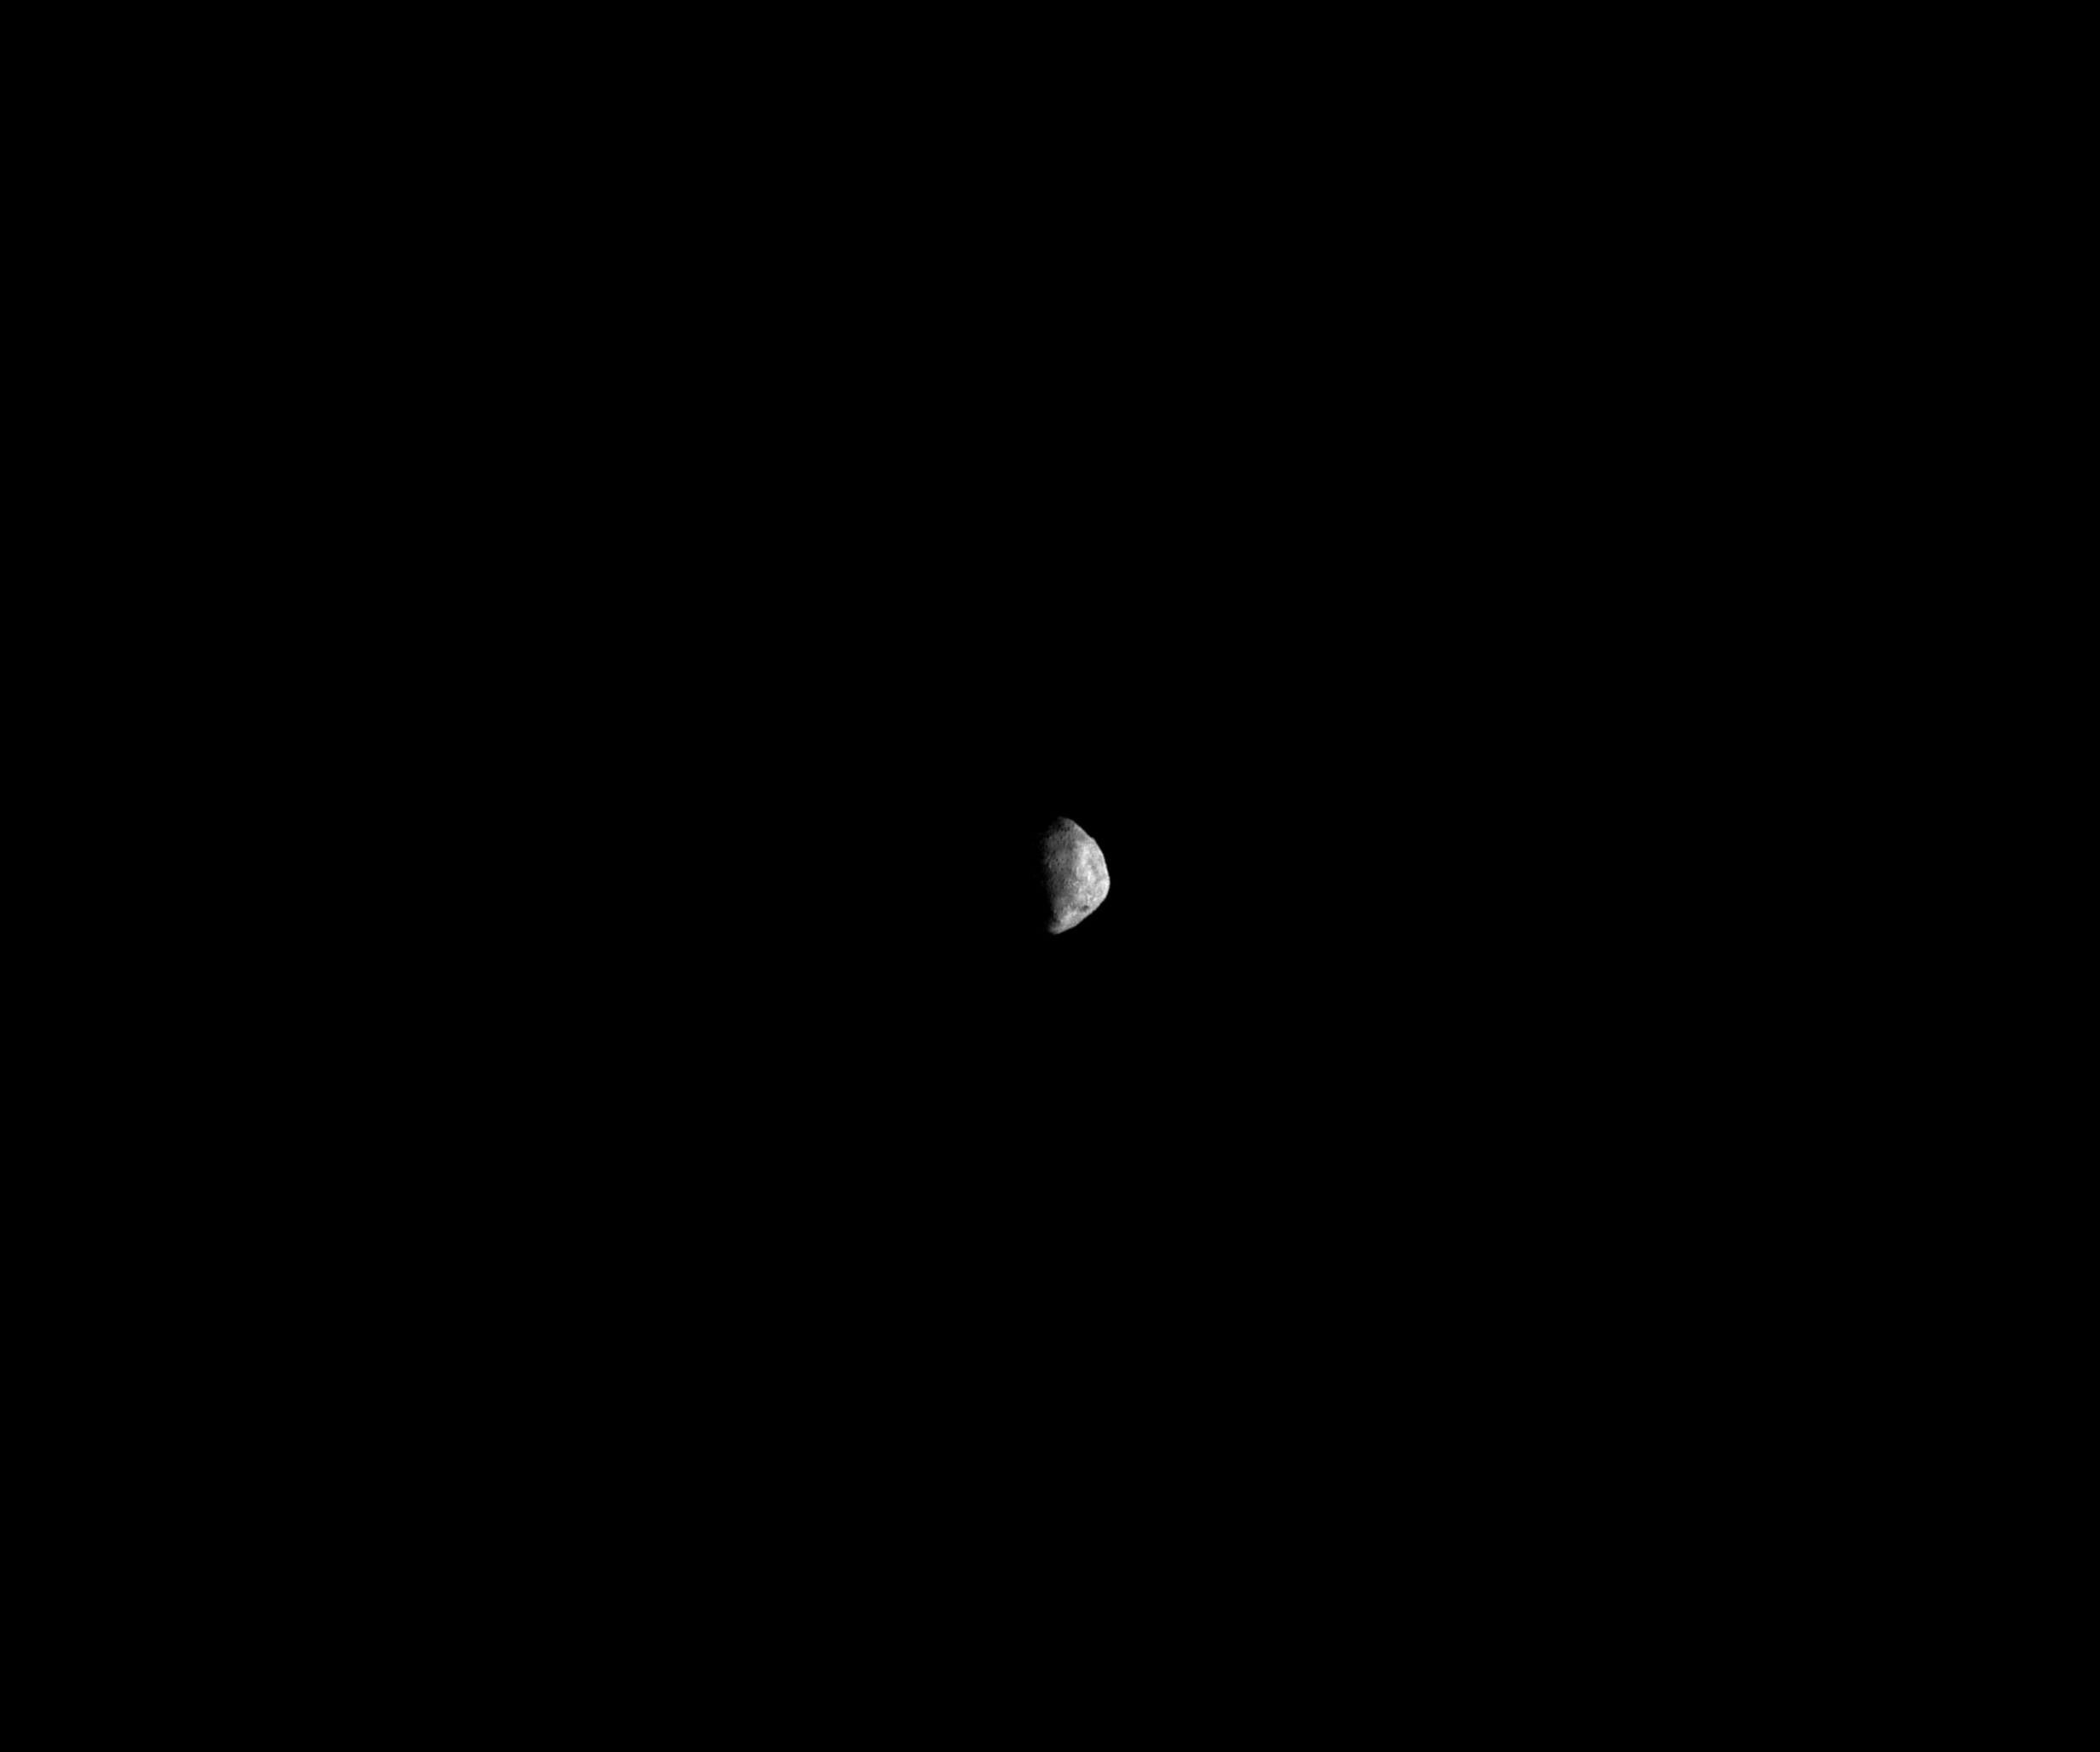
\includegraphics[width=\textwidth]{doc/thesis/0_figures/composition_varying_brightness/Inst_2017-08-15T115803-901000.png}
%             \label{fig:composition_varying_1}
%         \end{subfigure}
%         \begin{subfigure}[b]{0.32\textwidth}
%             \centering
%             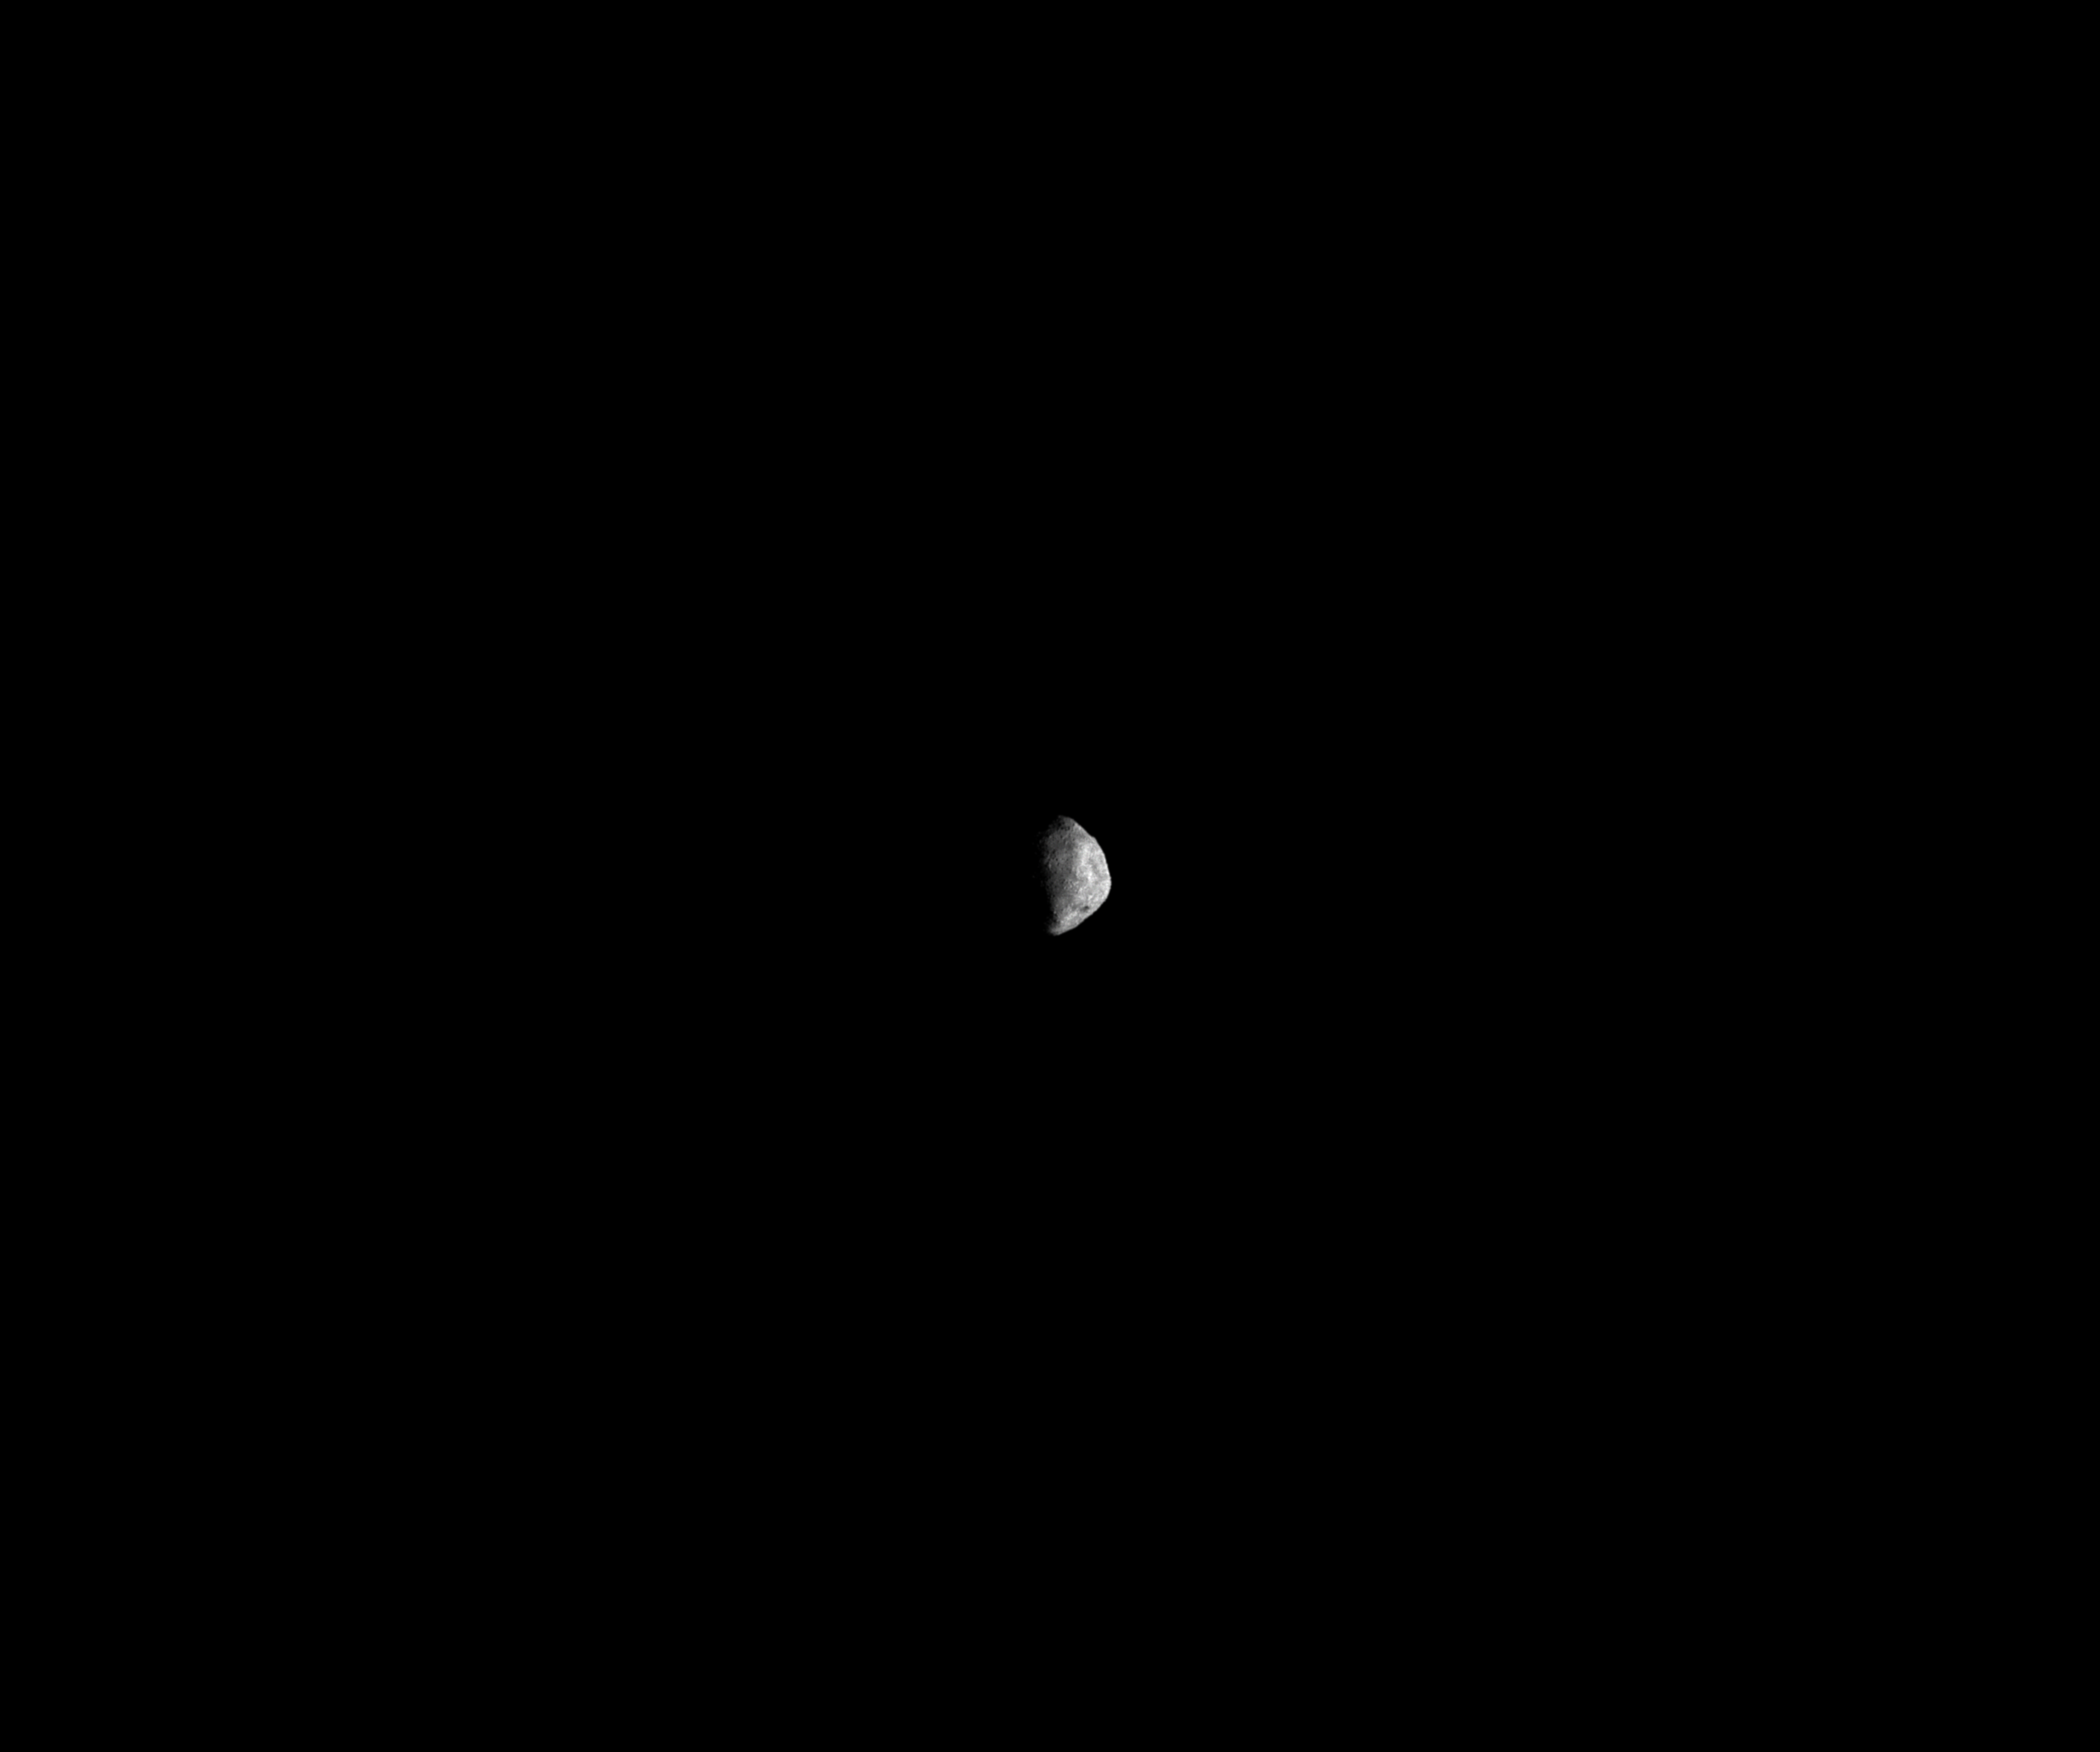
\includegraphics[width=\textwidth]{doc/thesis/0_figures/composition_varying_brightness/Inst_2017-08-15T115804-908000.png}
%             \label{fig:composition_varying_2}
%         \end{subfigure}
%         \begin{subfigure}[b]{0.32\textwidth}
%             \centering
%             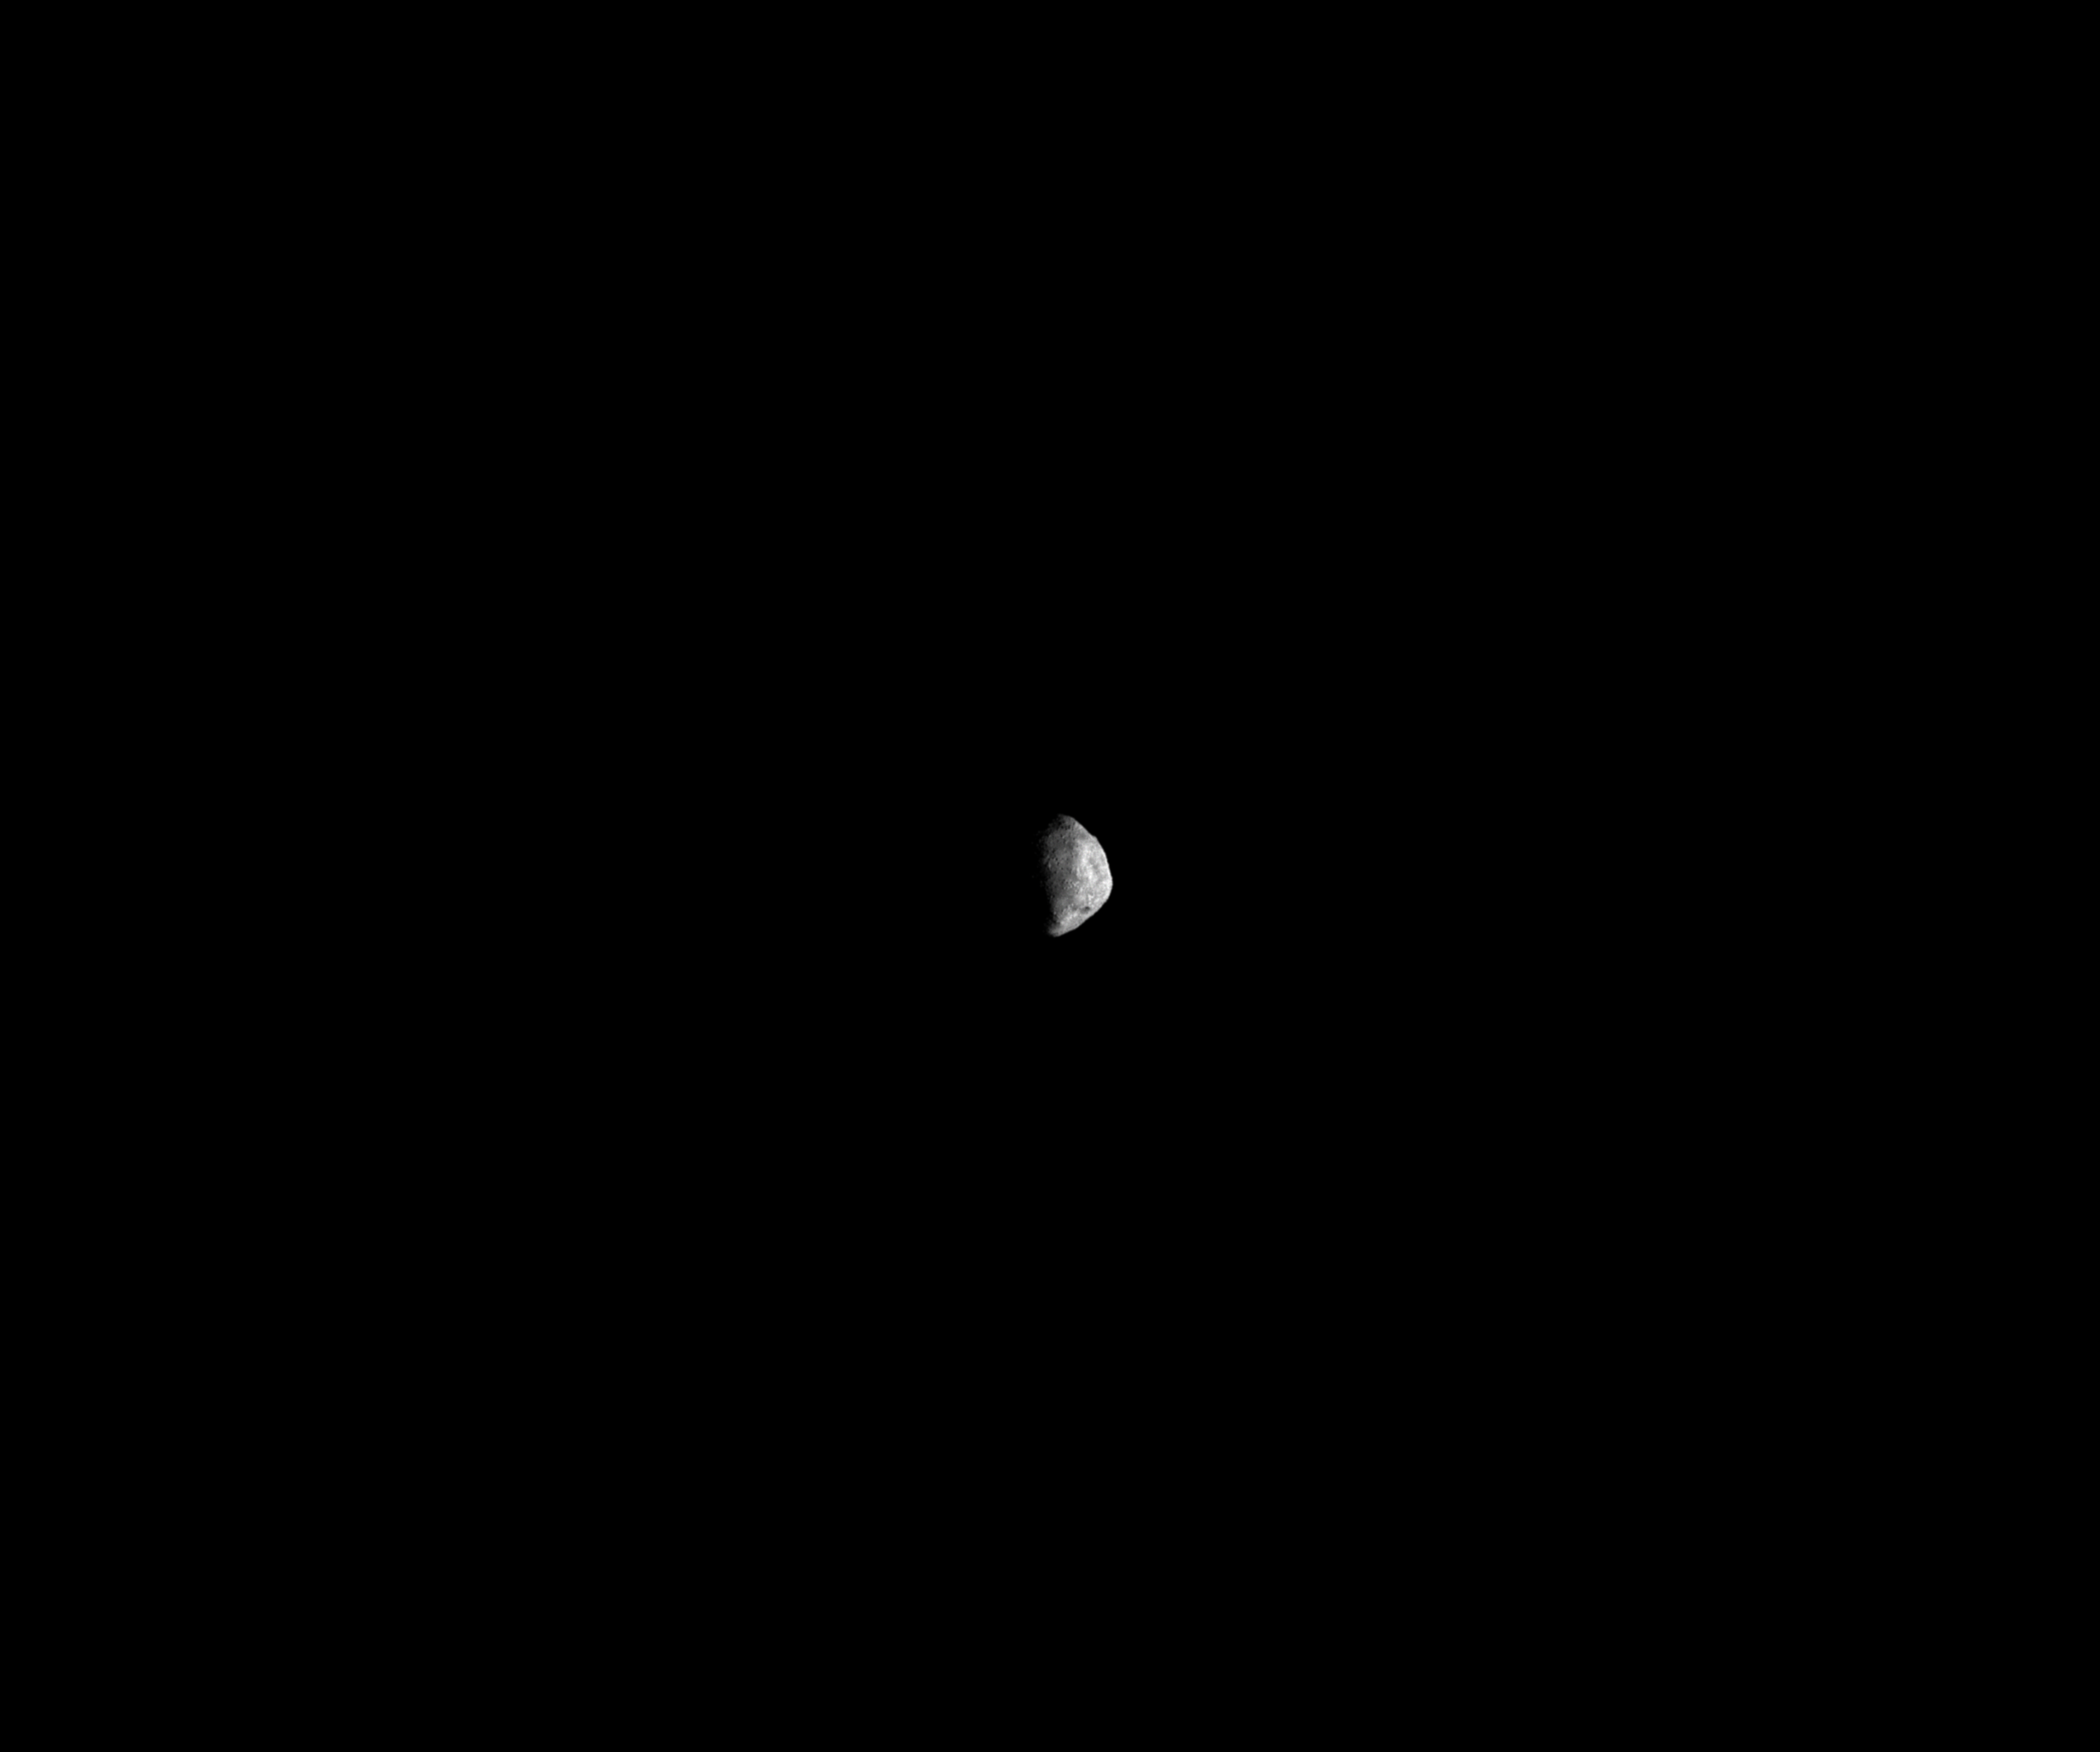
\includegraphics[width=\textwidth]{doc/thesis/0_figures/composition_varying_brightness/Inst_2017-08-15T115805-915000.png}
%             \label{fig:composition_varying_3}
%         \end{subfigure}
%     \caption{Varying brightness of patches on the \gls{sssb} surface.}
%     \label{fig:composition_varying}
% \end{figure}

\subsubsection{Rendering Problems} \label{sec:render_problems}
Rendering a fly-by scenario with a \SI{10}{\kilo\meter} \gls{sssb} created artefacts in the images. Figure~\ref{fig:render_artefacts} shows renders from fly-bys with different closest distances from the nucleus. All three images are the raw output from rendering, before composition. The images show a stripe, a darker patch across the \gls{sssb} with sharp brightness transitions. Moreover, the stripe is at the same location across the \gls{sssb} in all three images. This type of artefact does not appear for other \gls{sssb} sizes and not in all images with a \SI{10}{\kilo\meter} \gls{sssb}. The most likely explanation are errors while scaling the nucleus from the original \SI{1}{\kilo\meter} to the \SI{10}{\kilo\meter} model.
\begin{figure}[htb]
    \centering
    \begin{subfigure}[b]{0.32\textwidth}
        \centering
        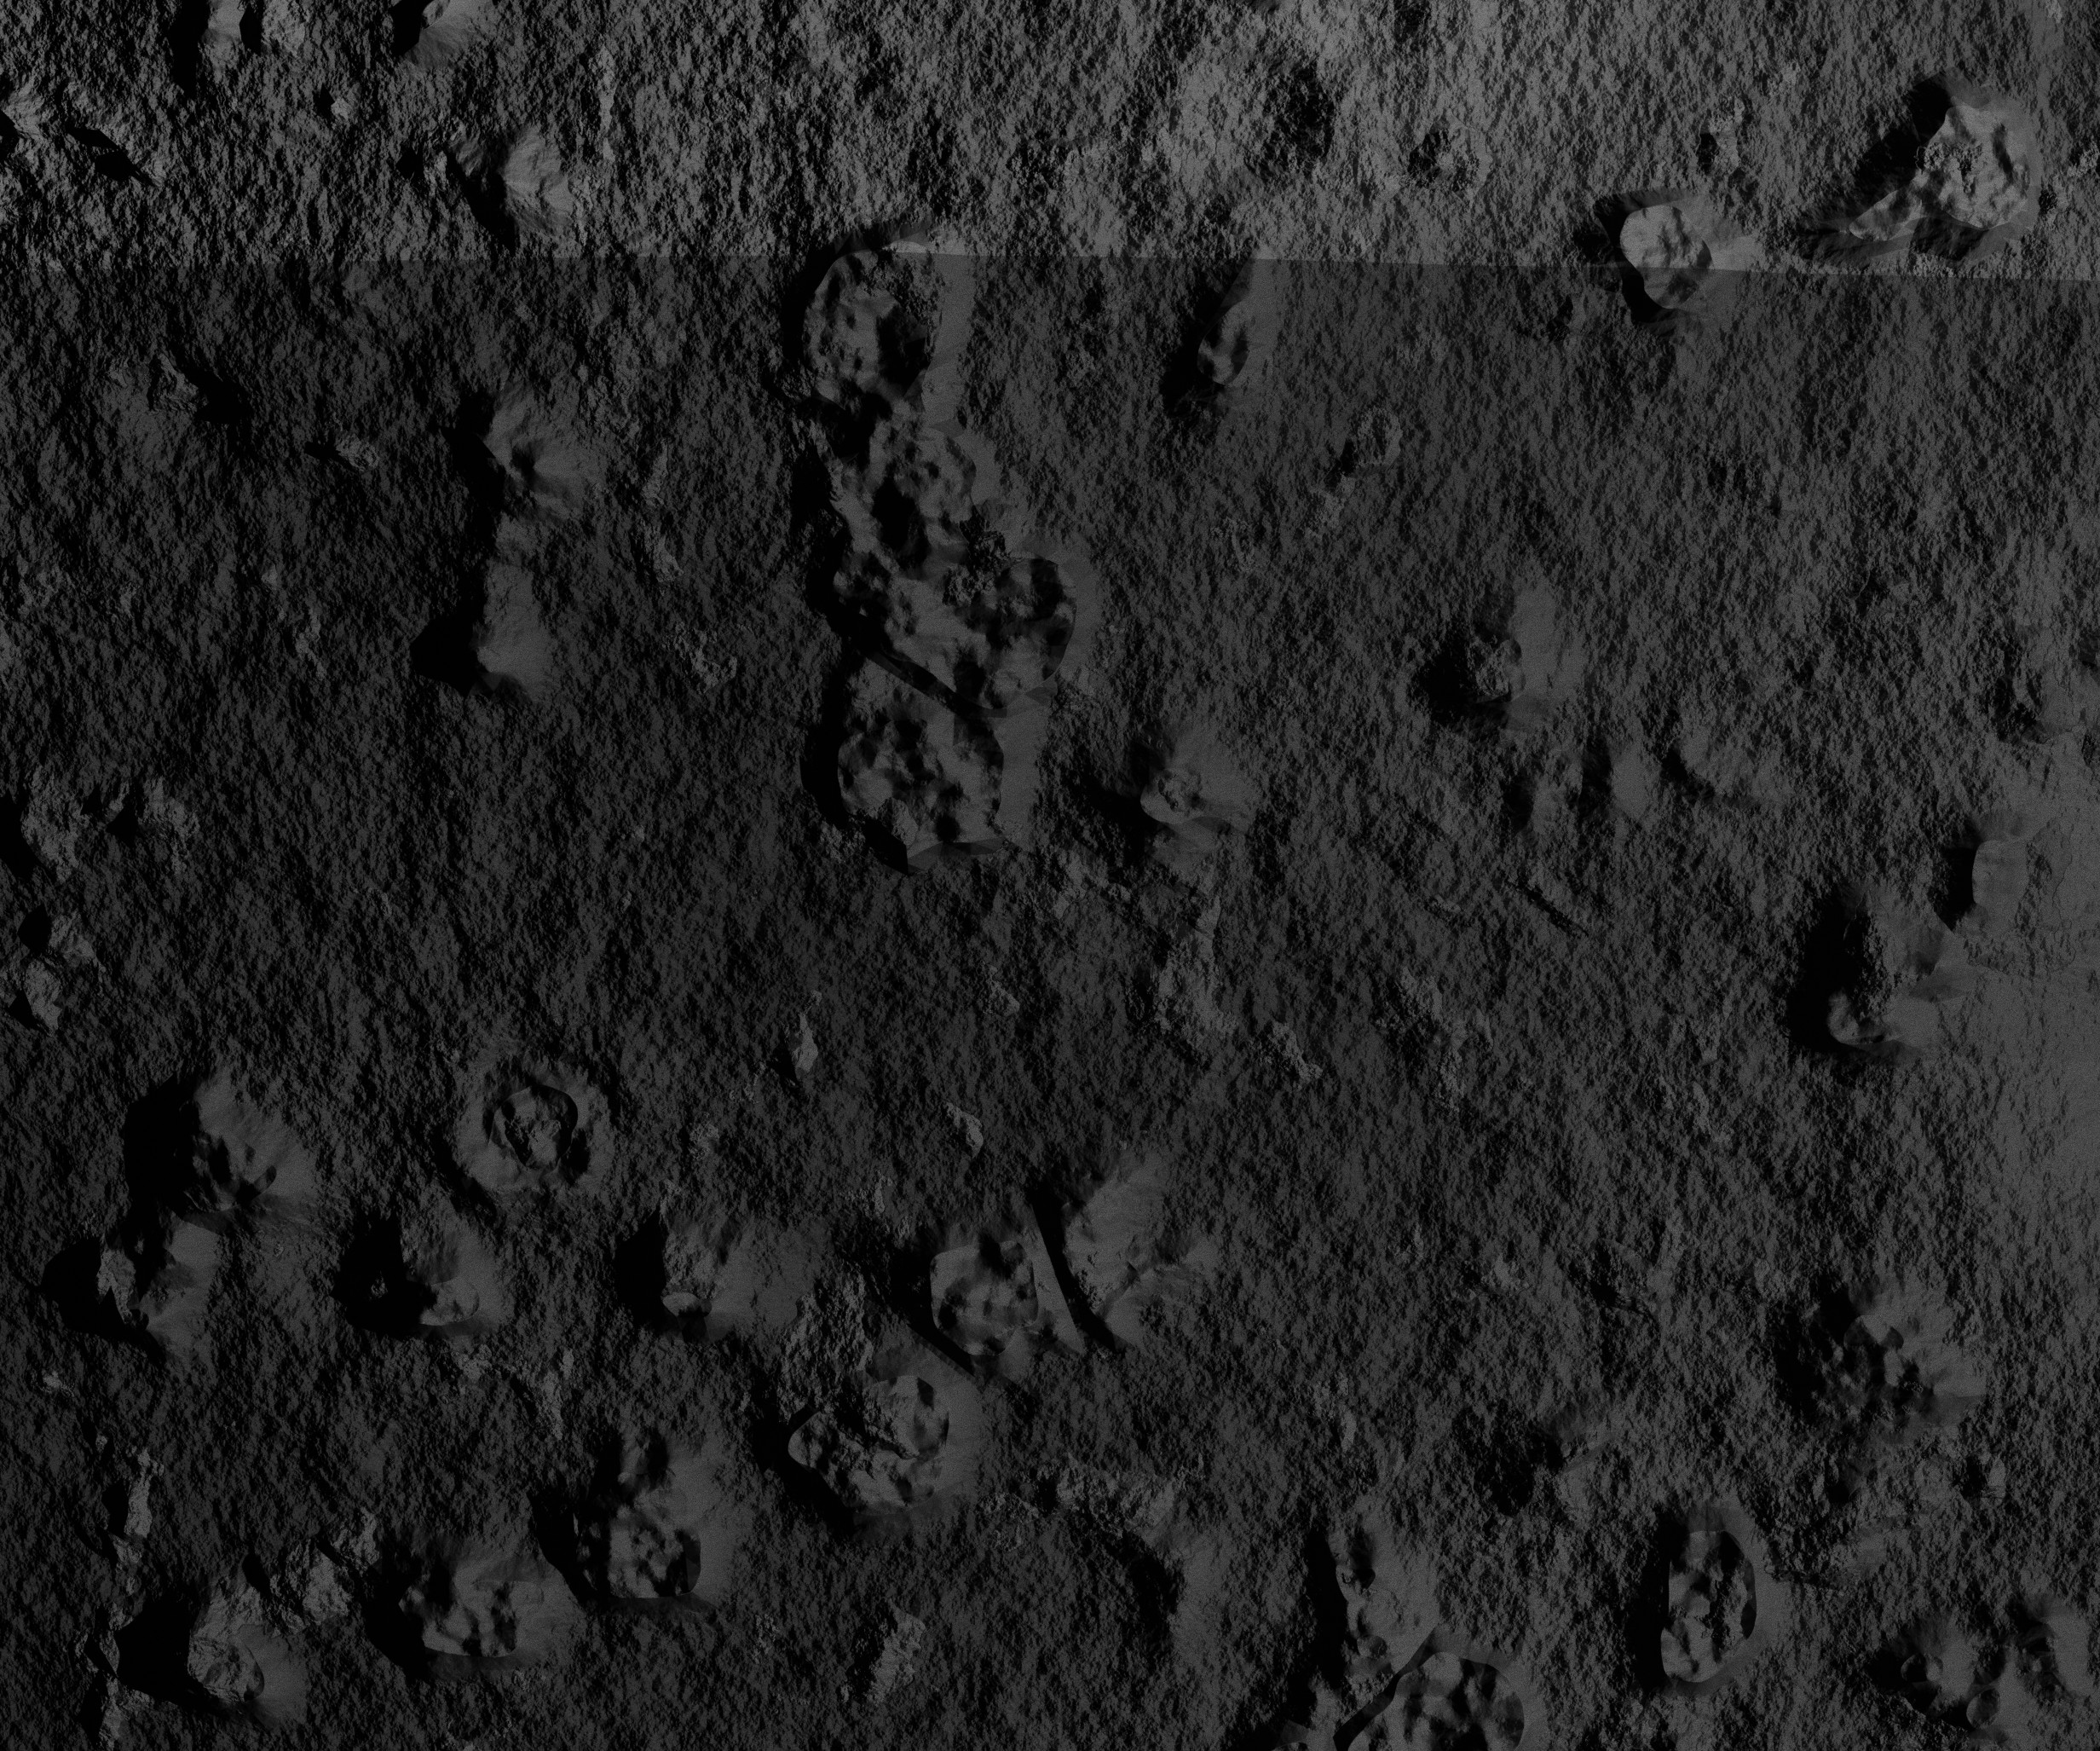
\includegraphics[width=\textwidth]{doc/thesis/0_figures/rendering_artefacts/50_10_SssbOnly_2017-08-15T115845-190000.jpg}
        \caption{}
        \label{fig:render_artefacts_50}
    \end{subfigure}
    \begin{subfigure}[b]{0.32\textwidth}
        \centering
        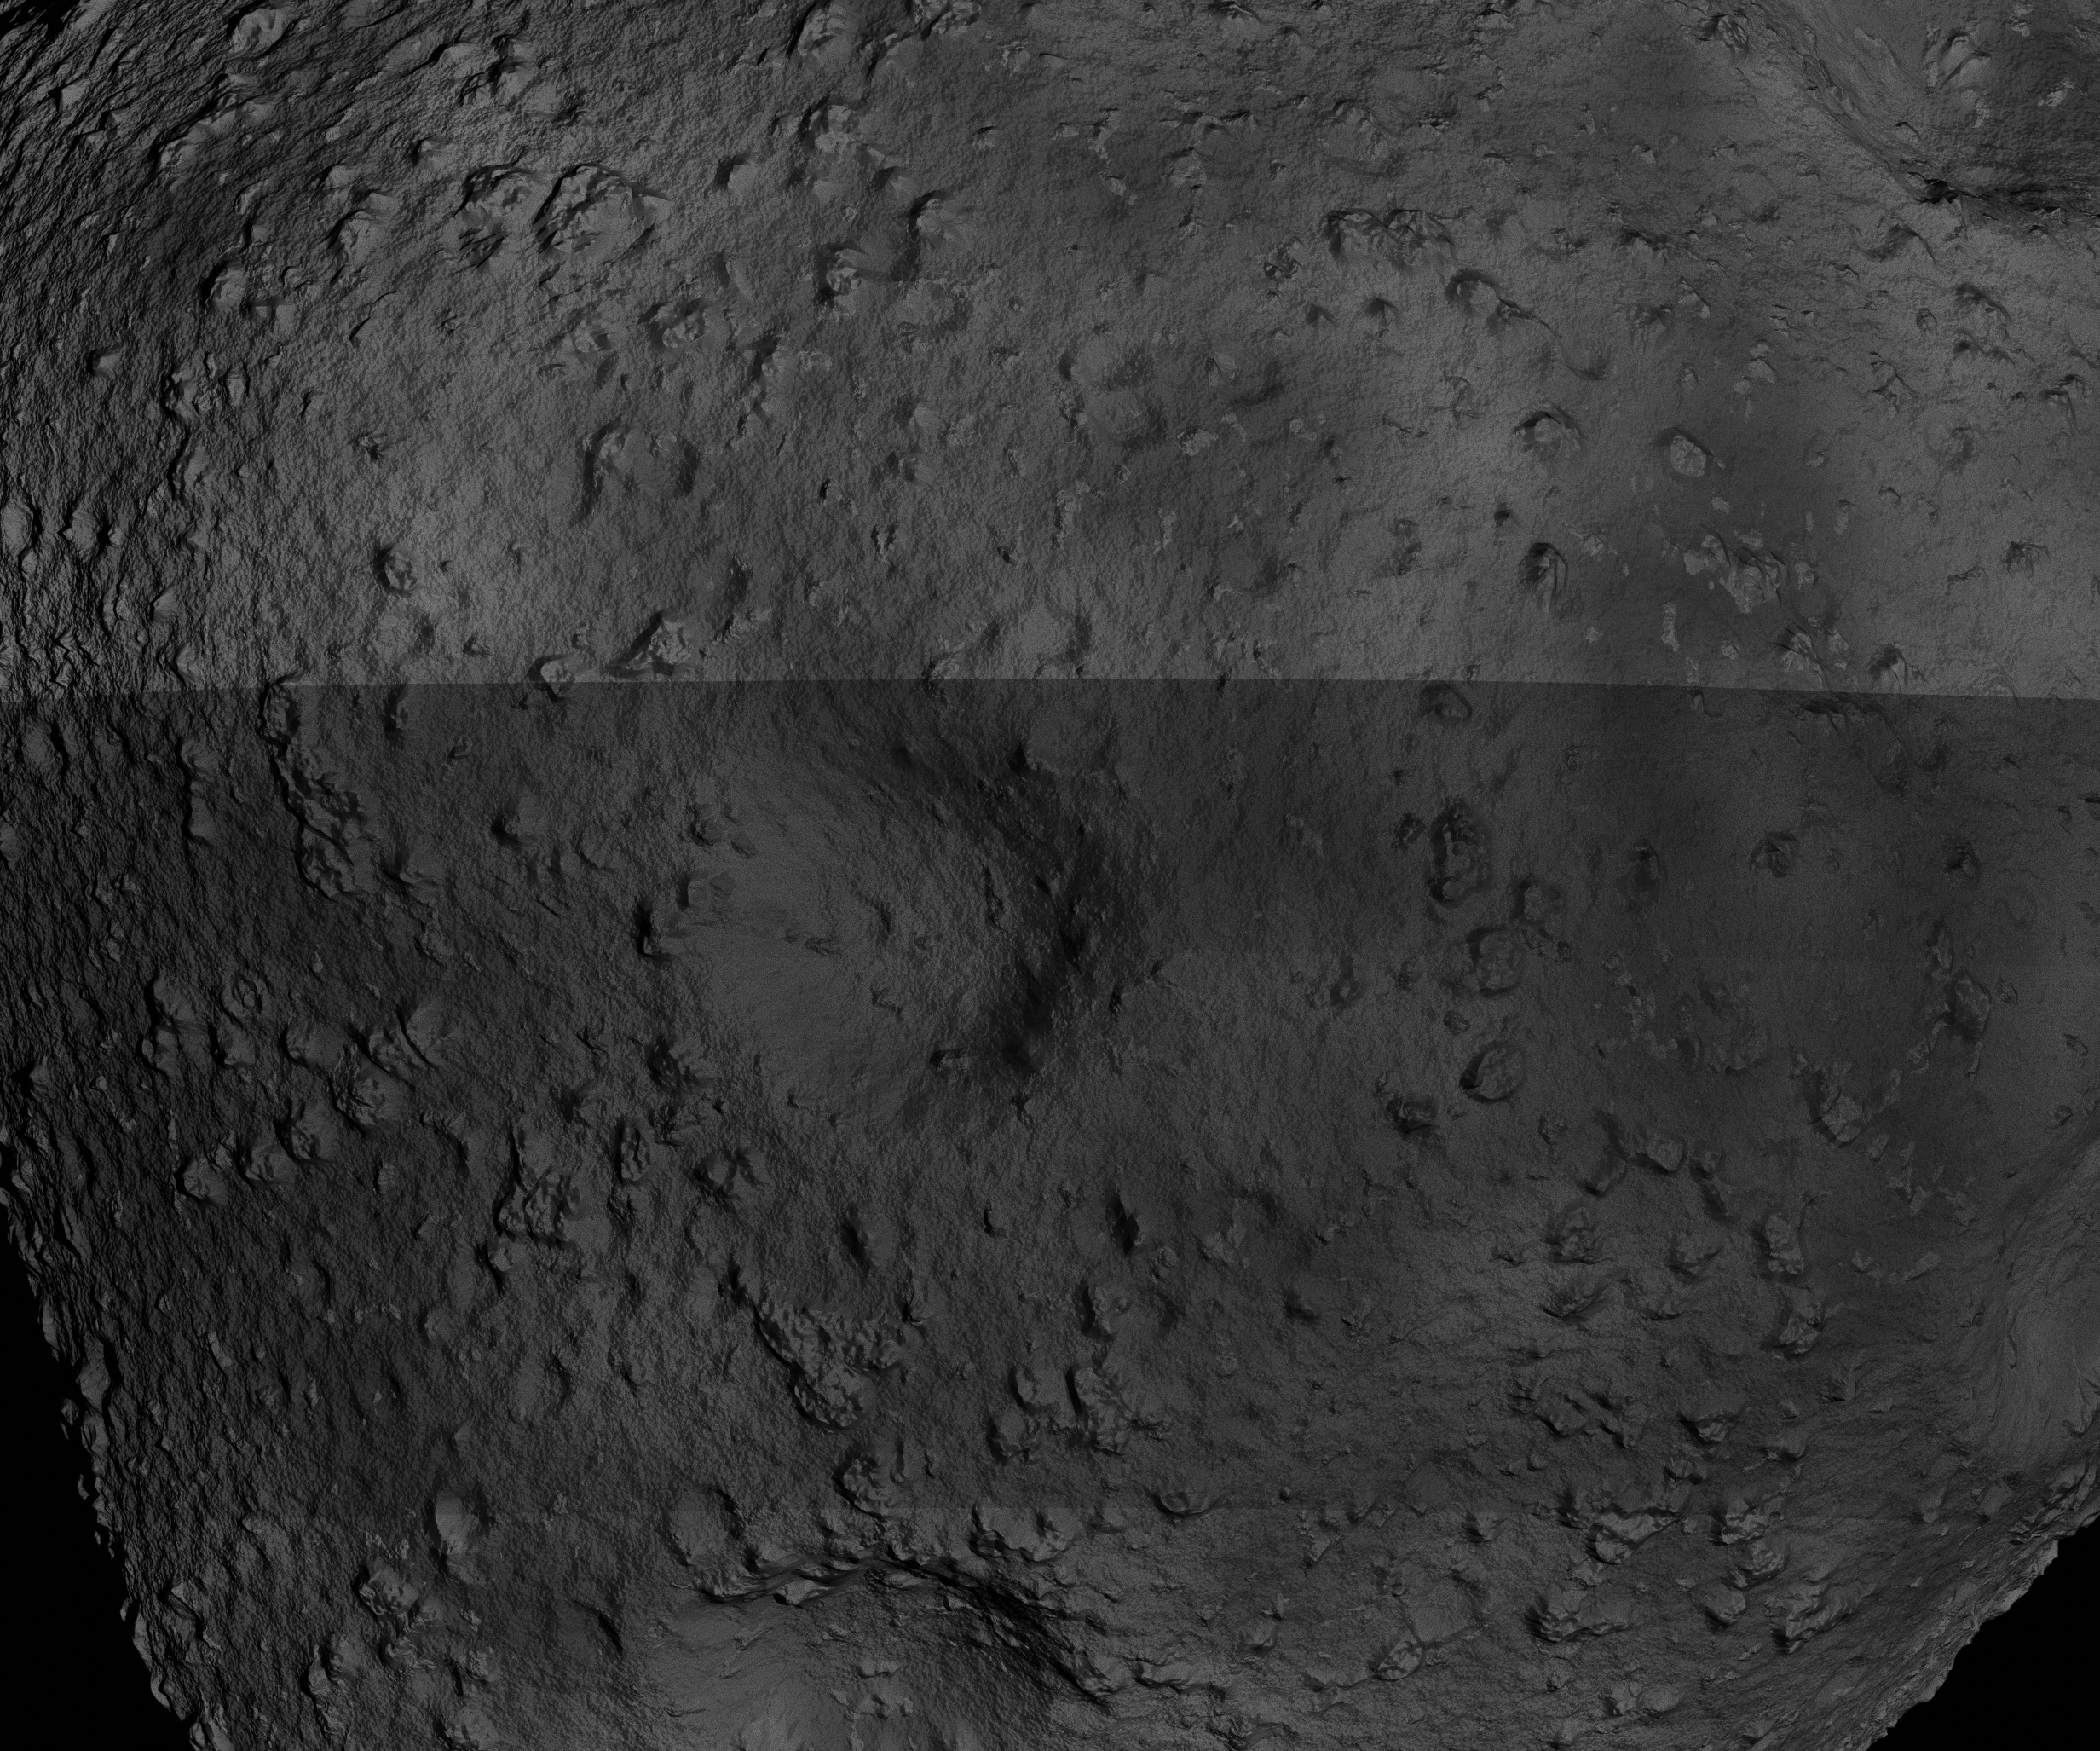
\includegraphics[width=\textwidth]{doc/thesis/0_figures/rendering_artefacts/200_10_SssbOnly_2017-08-15T115845-190000.jpg}
        \caption{}
        \label{fig:render_artefacts_200}
    \end{subfigure}
    \begin{subfigure}[b]{0.32\textwidth}
        \centering
        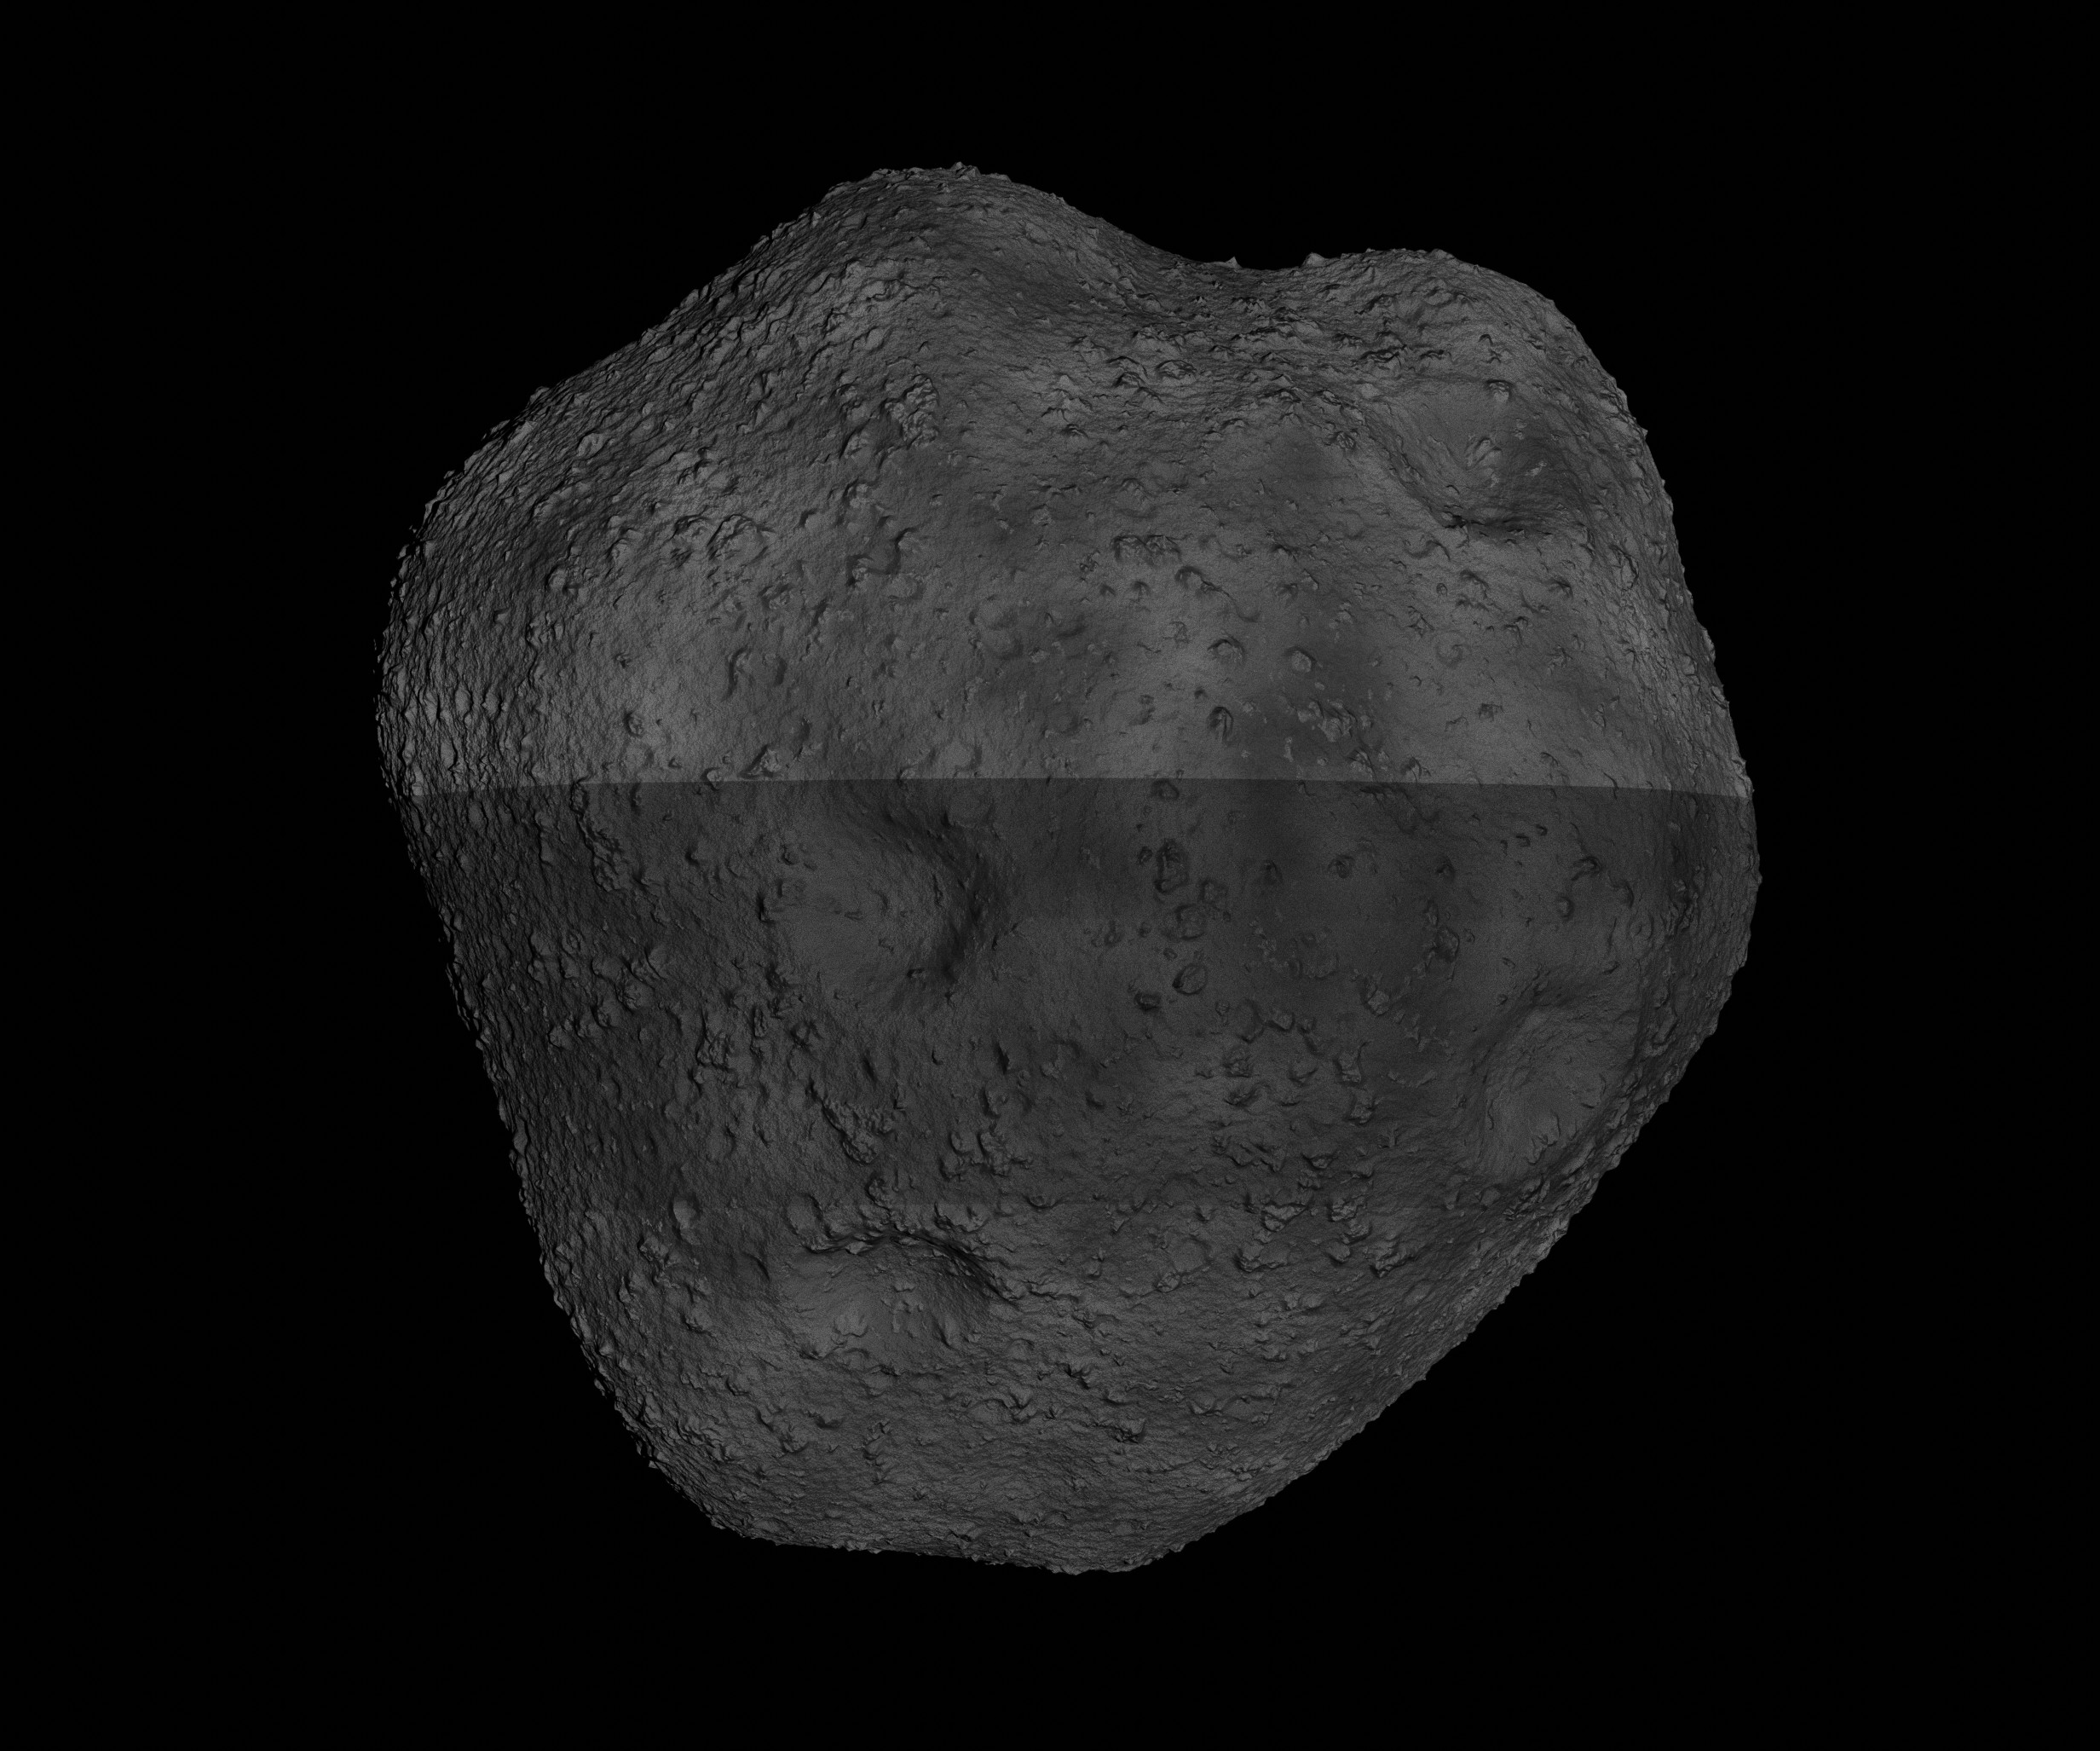
\includegraphics[width=\textwidth]{doc/thesis/0_figures/rendering_artefacts/400_10_SssbOnly_2017-08-15T115845-190000.jpg}
        \caption{}
        \label{fig:render_artefacts_400}
    \end{subfigure}
    \caption{Surface of a \SI{10}{\kilo\meter} \gls{sssb} for varying fly-by distances. Rendering artefacts, the stripes, are clearly visible in all three images. (a)~Closest-approach \SI{50}{\kilo\meter}. (b)~Closest-approach \SI{200}{\kilo\meter}. (c)~Closest-approach \SI{400}{\kilo\meter}.}
    \label{fig:render_artefacts}
\end{figure}

A second problem occurred in a \SI{50}{\kilo\meter} fly-by simulation with a \SI{1}{\kilo\meter} \gls{sssb}. A single image was found to be darker than all other images in the data set. Figure~\ref{fig:render_dark} shows three images where the middle image is overall darker except for one small patch of white pixels. Three pixels are much brighter than any other pixel in the image. These are so-called \textit{fireflies}~\cite{Valenza2015BlenderCookbook}. Figure~\ref{fig:render_dark} contains composed images for better visibility of the artefact. The artefact is not introduced by the composition process since it exists in the raw rendered images. No second image with the same issue was found in any other data set therefore the problem was not investigated further.

\begin{figure}[htb]
    \centering
        \begin{subfigure}[b]{0.32\textwidth}
            \centering
            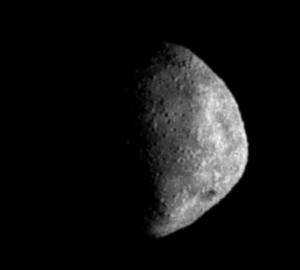
\includegraphics[width=\textwidth]{doc/thesis/0_figures/composition_darkening/50km_Inst_2017-08-15T115816-993000_center.png}
            \label{fig:render_dark_1}
        \end{subfigure}
        \begin{subfigure}[b]{0.32\textwidth}
            \centering
            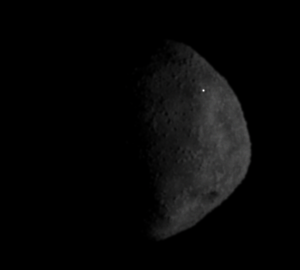
\includegraphics[width=\textwidth]{doc/thesis/0_figures/composition_darkening/Inst_2017-08-15T115818-000000_center.png}
            \label{fig:render_dark_2}
        \end{subfigure}
        \begin{subfigure}[b]{0.32\textwidth}
            \centering
            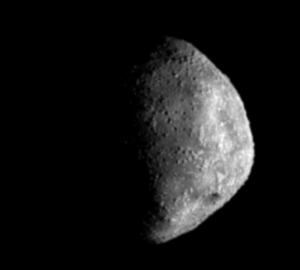
\includegraphics[width=\textwidth]{doc/thesis/0_figures/composition_darkening/Inst_2017-08-15T115819-007000_center.png}
            \label{fig:render_dark_3}
        \end{subfigure}
    \caption{Overall darkened \gls{sssb} image due to three pixels being much brighter. These pixels are referred to as fireflies. All three images are composed images for better visibility of the artefact. The images are cropped to display the \gls{sssb} nucleus and artefact better.}
    \label{fig:render_dark}
\end{figure}

\clearpage

\subsection{Compression} \label{sec:results_comp}
The \gls{sispo} software package was used to study the effects of compression in different scenarios. The scenarios are presented in Table~\ref{tab:sim_params}. Two compression algorithms were used to study compression effects. The \gls{png} format was used because of its wide support among different software packages and \gls{jp2} is used as an improved version over commonly used \gls{jpeg}. The \gls{png} and \gls{jp2} formats were selected as general examples to characterise the compression effects on reconstruction. Neither of these two algorithms is intended to represent image processing on-board a spacecraft. Scenarios with varying \gls{sssb} nucleus sizes and fly-by distance were simulated. 
Comparison of the different compression algorithms is based on several output parameters. The data size of the compressed image series, the number of points in the dense reconstructed point cloud, the number of vertices and the number of faces of the refined reconstructed model. These outputs relate well to the level of detail of the rendered images, since \gls{sfm} algorithms rely on surface details for reconstruction.

\subsubsection{Image Quality Comparison} \label{sec:img_quali_comp}
To compare the image quality after different levels of compression, a specific image is selected which is compressed to different levels. Since reconstruction is mostly influenced by features, a scene with a distance of \SI{50}{\kilo\meter} was selected for comparison. Once the overall images, containing the entire \gls{sssb} in the \gls{fov}, and closeups, highlighted by the red frame in Figure~\ref{fig:img_quality_frame} are studied. Overall images are used to show compression effects on an entire scene while the closeup images reveal compression effects on surface details. Difference images and histograms are used to further investigate the effects of compression. Difference images are created by converting the \gls{rgb} images to greyscale and taking the L2-norm after subtracting each pixel from the respective value of the \gls{png} greyscale image. The result is a greyscale difference image showing the L2-norm differences. For the histograms, the zero values were removed to only show differences. Therefore, the total number of pixels and the percentage compared to the original that were used for the histogram are given as well.

\begin{figure}[htb]
    \centering
    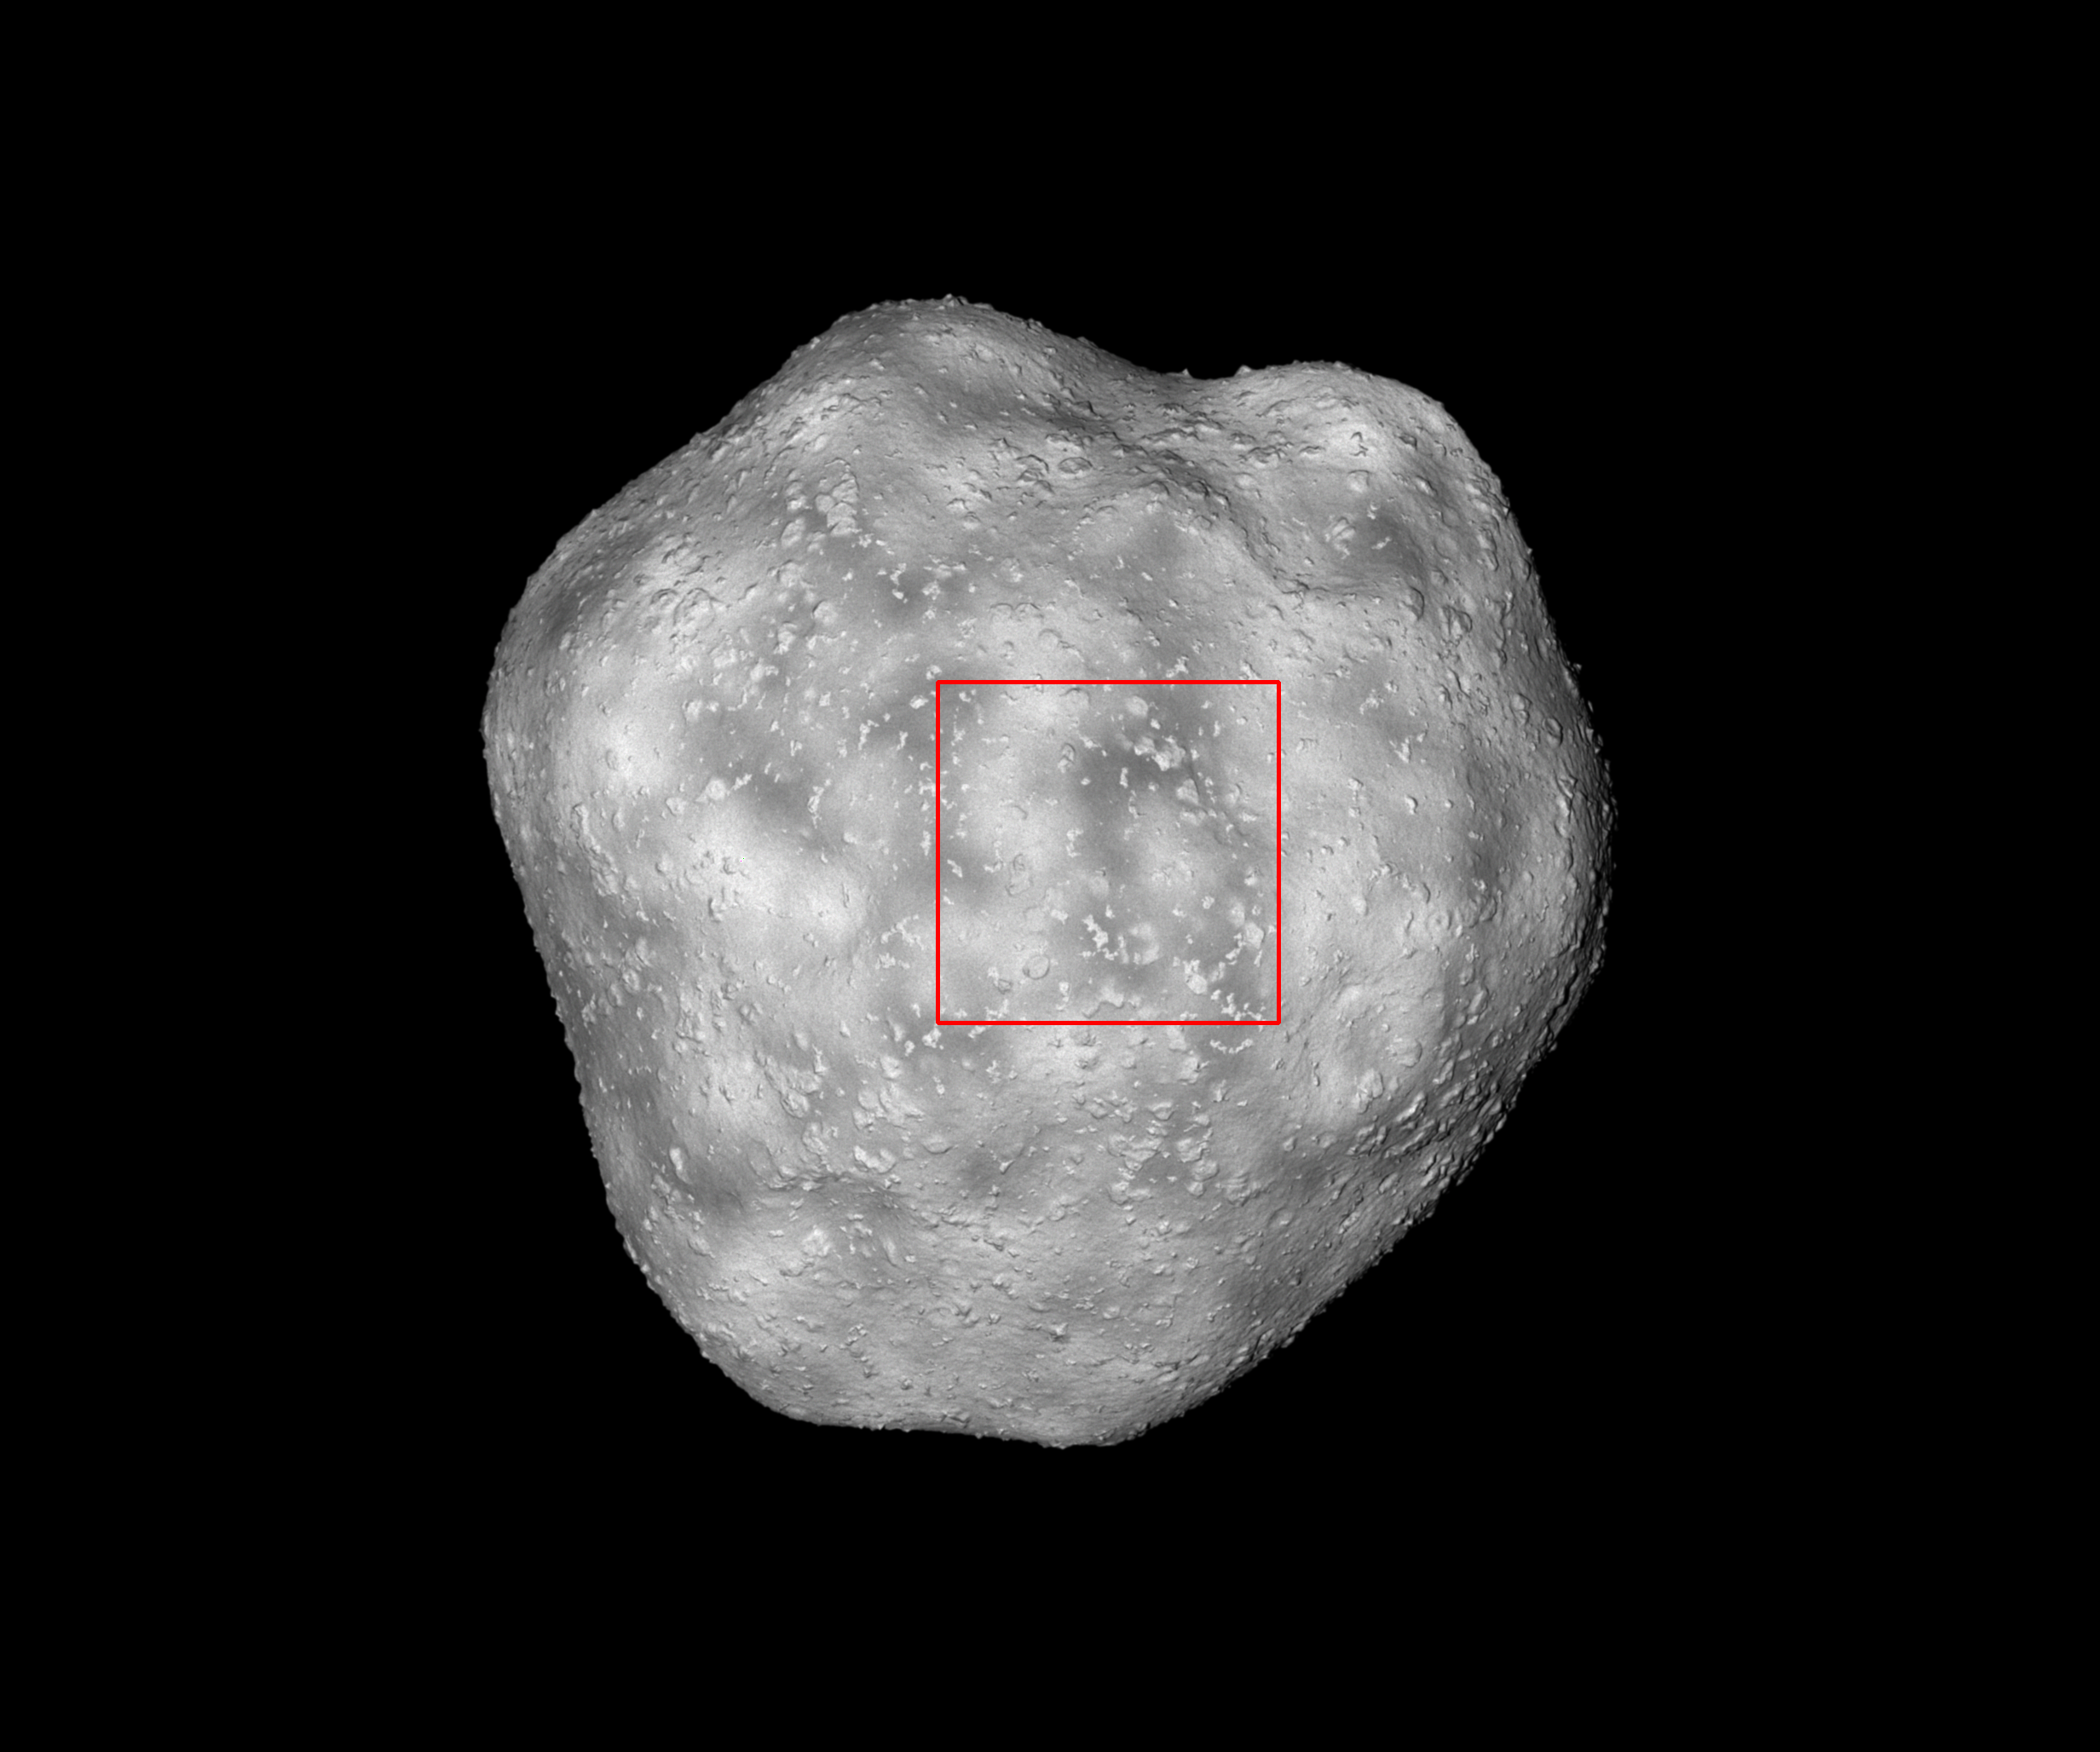
\includegraphics[width=.7\textwidth]{doc/thesis/0_figures/compare_quality/set1/jp2_1000_frame}
    \caption{Scene used for quality comparison. The area highlighted in red is studied up closer. The specific area was selected since it includes a wide range of colours and various sized surface features.}
    \label{fig:img_quality_frame}
\end{figure}

Figures~\ref{fig:img_quality_comp_jp2_1} to \ref{fig:img_quality_comp_jp2_1000} show the compressed overall image, the difference histograms as well as the difference images after compression with \gls{jp2} with quality levels \SI{1}{}, \SI{5}{}, \SI{10}{}, \SI{100}{} and \SI{1000}{}. Quality level \SI{5}{} is used since most changes due to compression occur at low quality levels.

\begin{figure}[htb]
    \centering
    \begin{subfigure}[b]{0.48\textwidth}
        \centering
        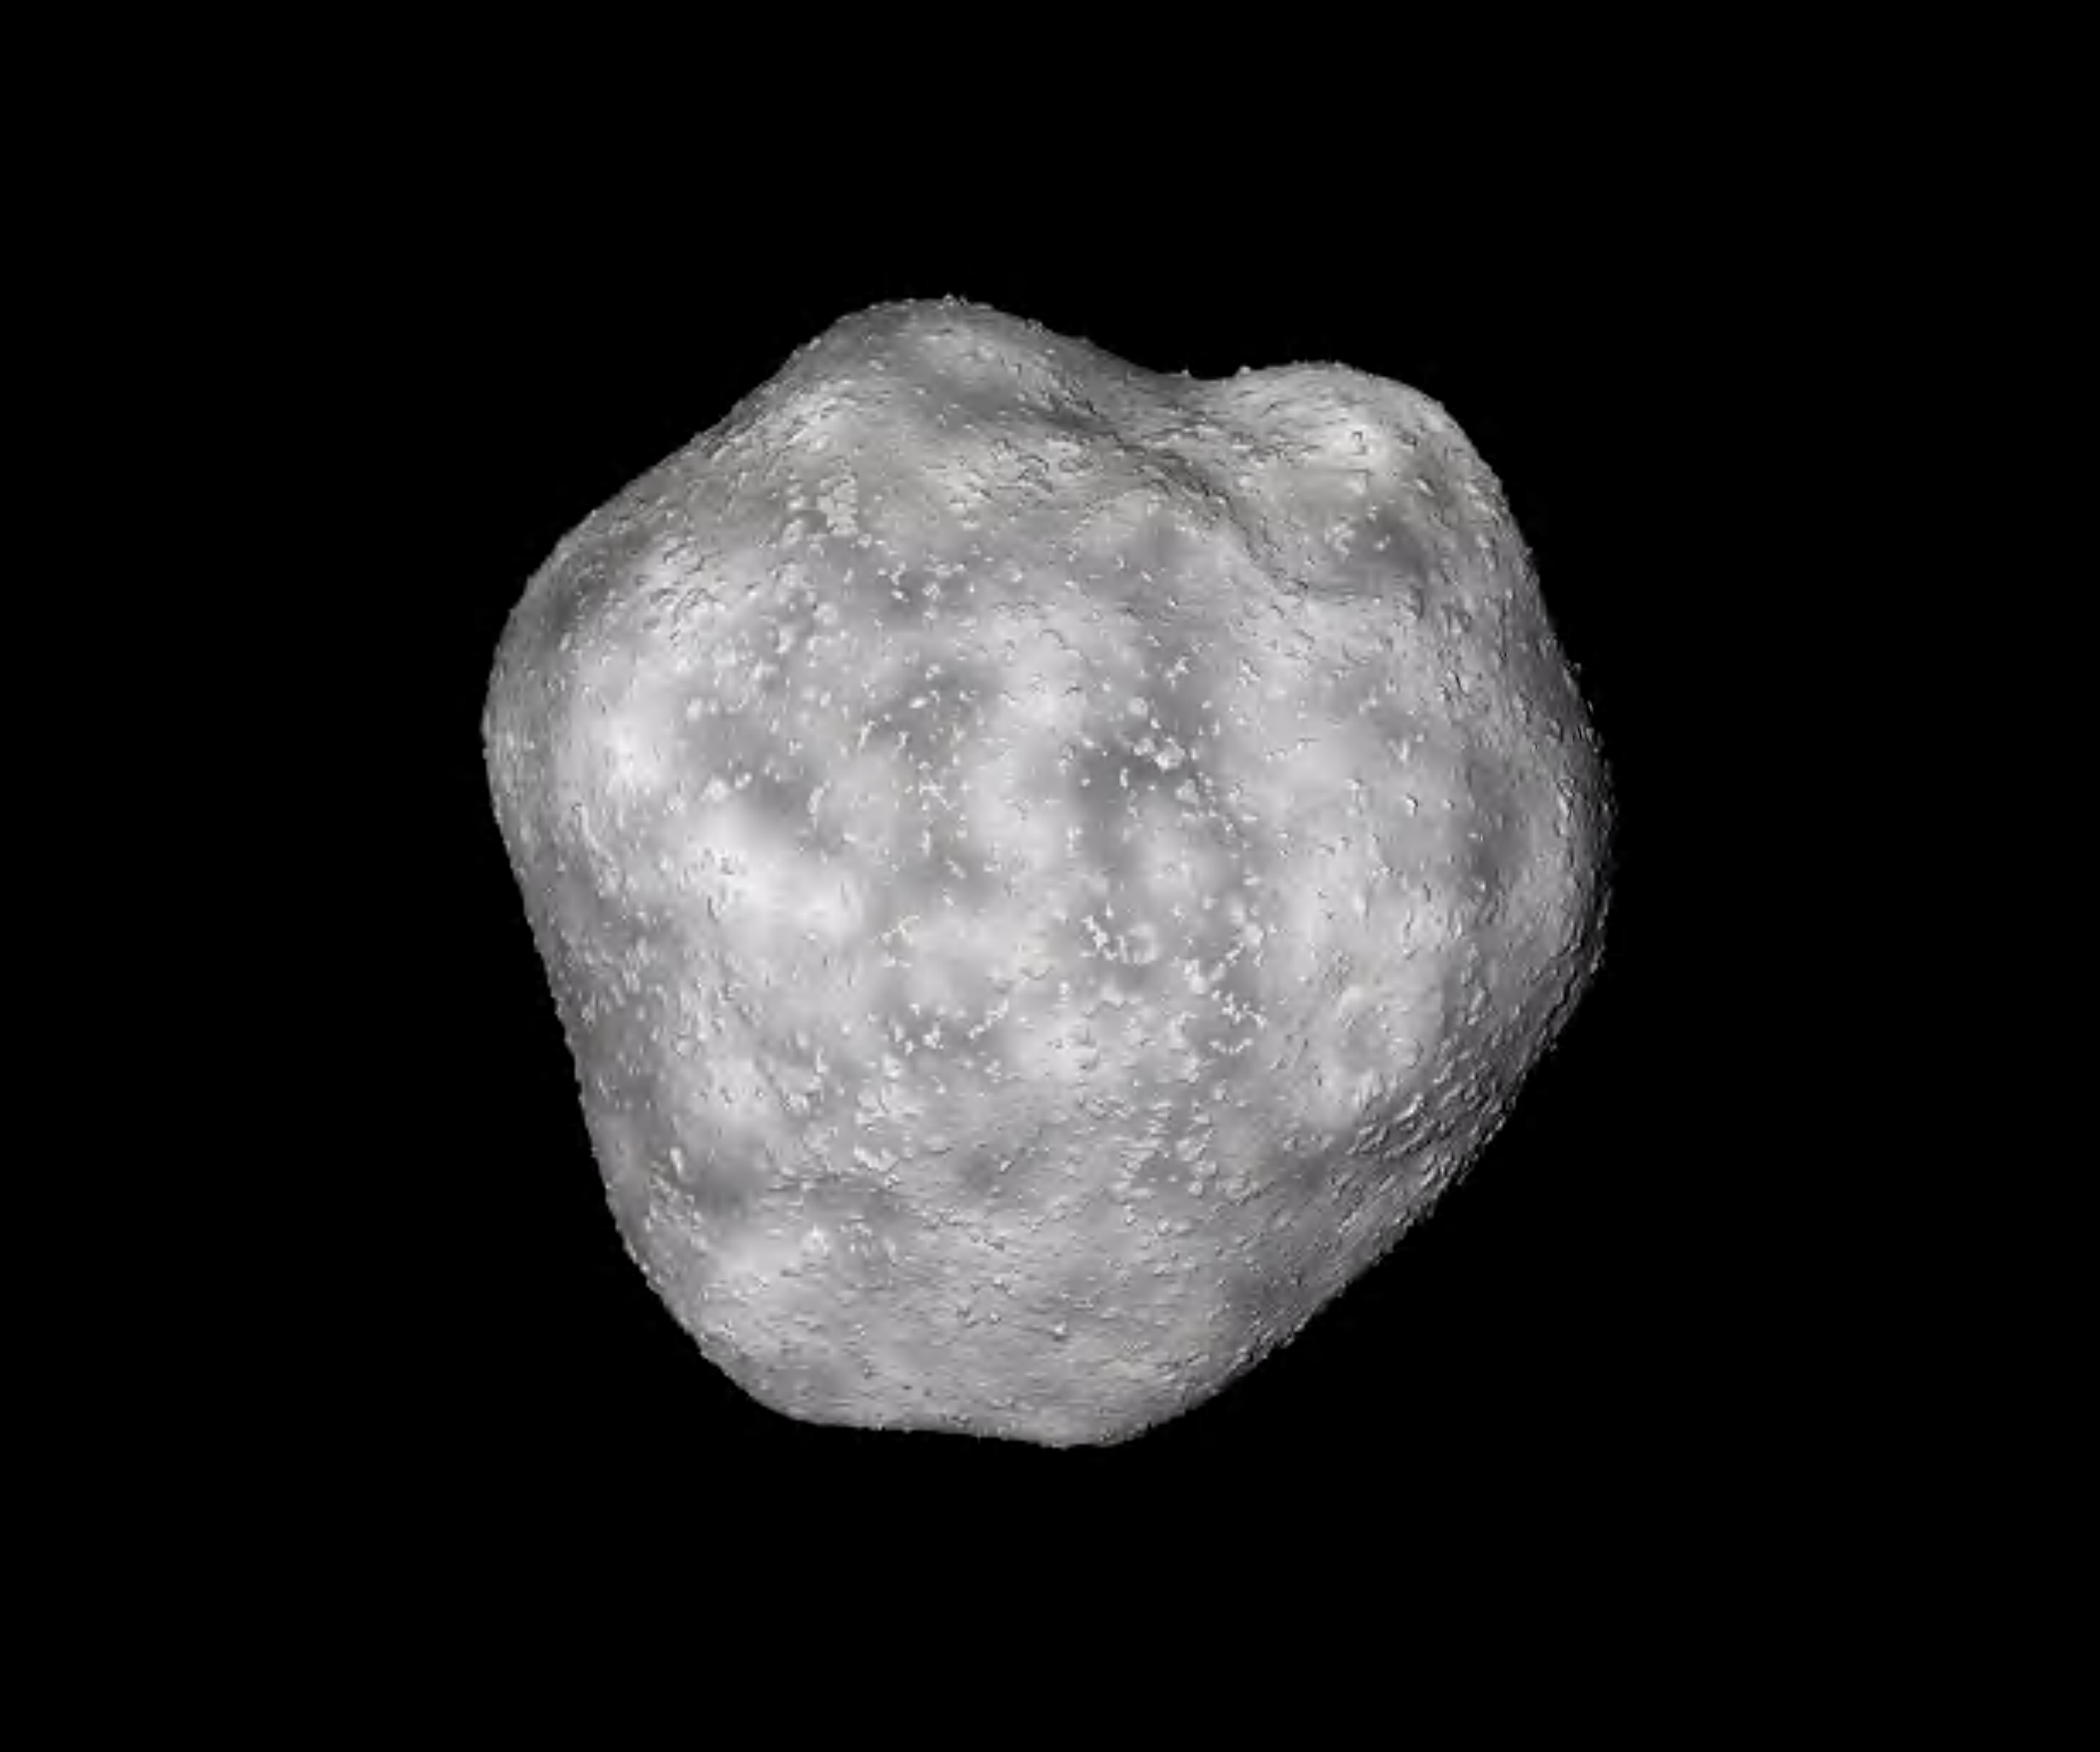
\includegraphics[width=\textwidth]{doc/thesis/0_figures/compare_quality/set1/jp2_1}
        \caption{}
        \label{fig:img_quality_comp_jp2_1_orig}
    \end{subfigure}
    \begin{subfigure}[b]{0.48\textwidth}
        \centering
        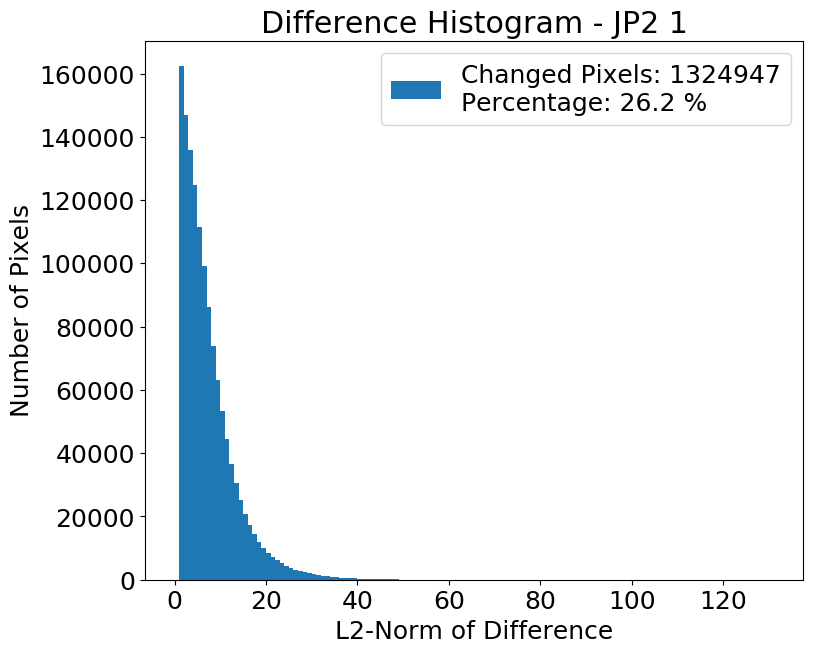
\includegraphics[width=\textwidth]{doc/thesis/0_figures/compare_quality/set1/jp2_1_diff_histogram}
        \caption{}
        \label{fig:img_quality_comp_jp2_1_histo}
    \end{subfigure}
    \\
    \begin{subfigure}[b]{0.48\textwidth}
        \centering
        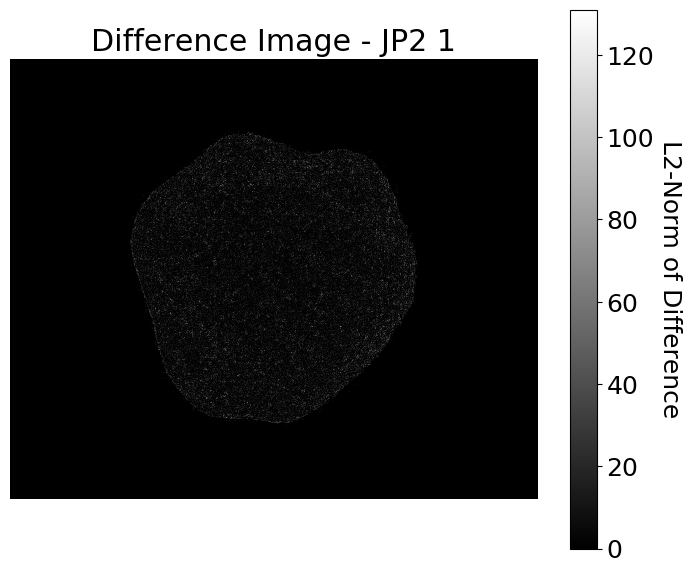
\includegraphics[width=\textwidth]{doc/thesis/0_figures/compare_quality/set1/jp2_1_diff_heatmap}
        \caption{}
        \label{fig:img_quality_comp_jp2_1_diff}
    \end{subfigure}
    \begin{subfigure}[b]{0.48\textwidth}
        \centering
        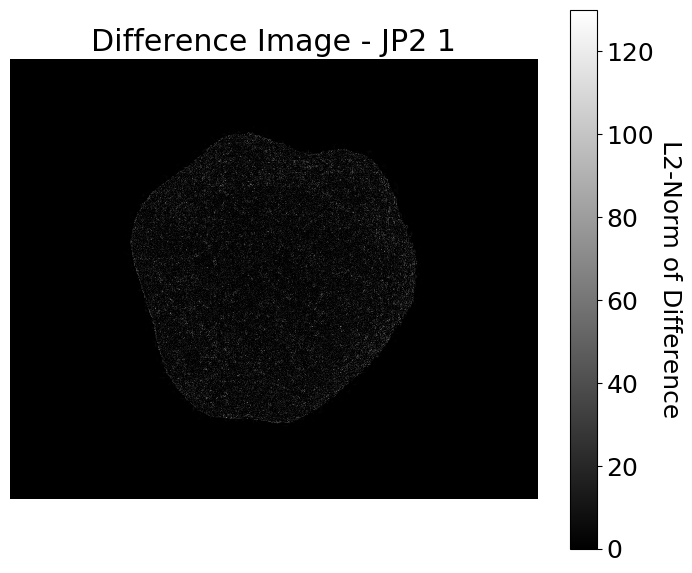
\includegraphics[width=\textwidth]{doc/thesis/0_figures/compare_quality/set1/jp2_1_diff_heatmap_rel}
        \caption{}
        \label{fig:img_quality_comp_jp2_1_diff_rel}
    \end{subfigure}
    \caption{Overall rendered image after compression with \gls{jp2} quality level 1. The L2-norm is applied to the difference between the greyscale images of the lossless and respective lossy image. (a) Image after lossy compression. (b) Histogram of L2-norms of differences. (c) L2-norm difference image with a colour scale from $0$ to $131$ for comparison between various compression levels. (d) L2-norm difference image with a colour scale from $0$ to the maximum L2-norm value for better visibility of compression effects.}
    \label{fig:img_quality_comp_jp2_1}
\end{figure}


\begin{figure}[htb]
    \centering
    \begin{subfigure}[b]{0.48\textwidth}
        \centering
        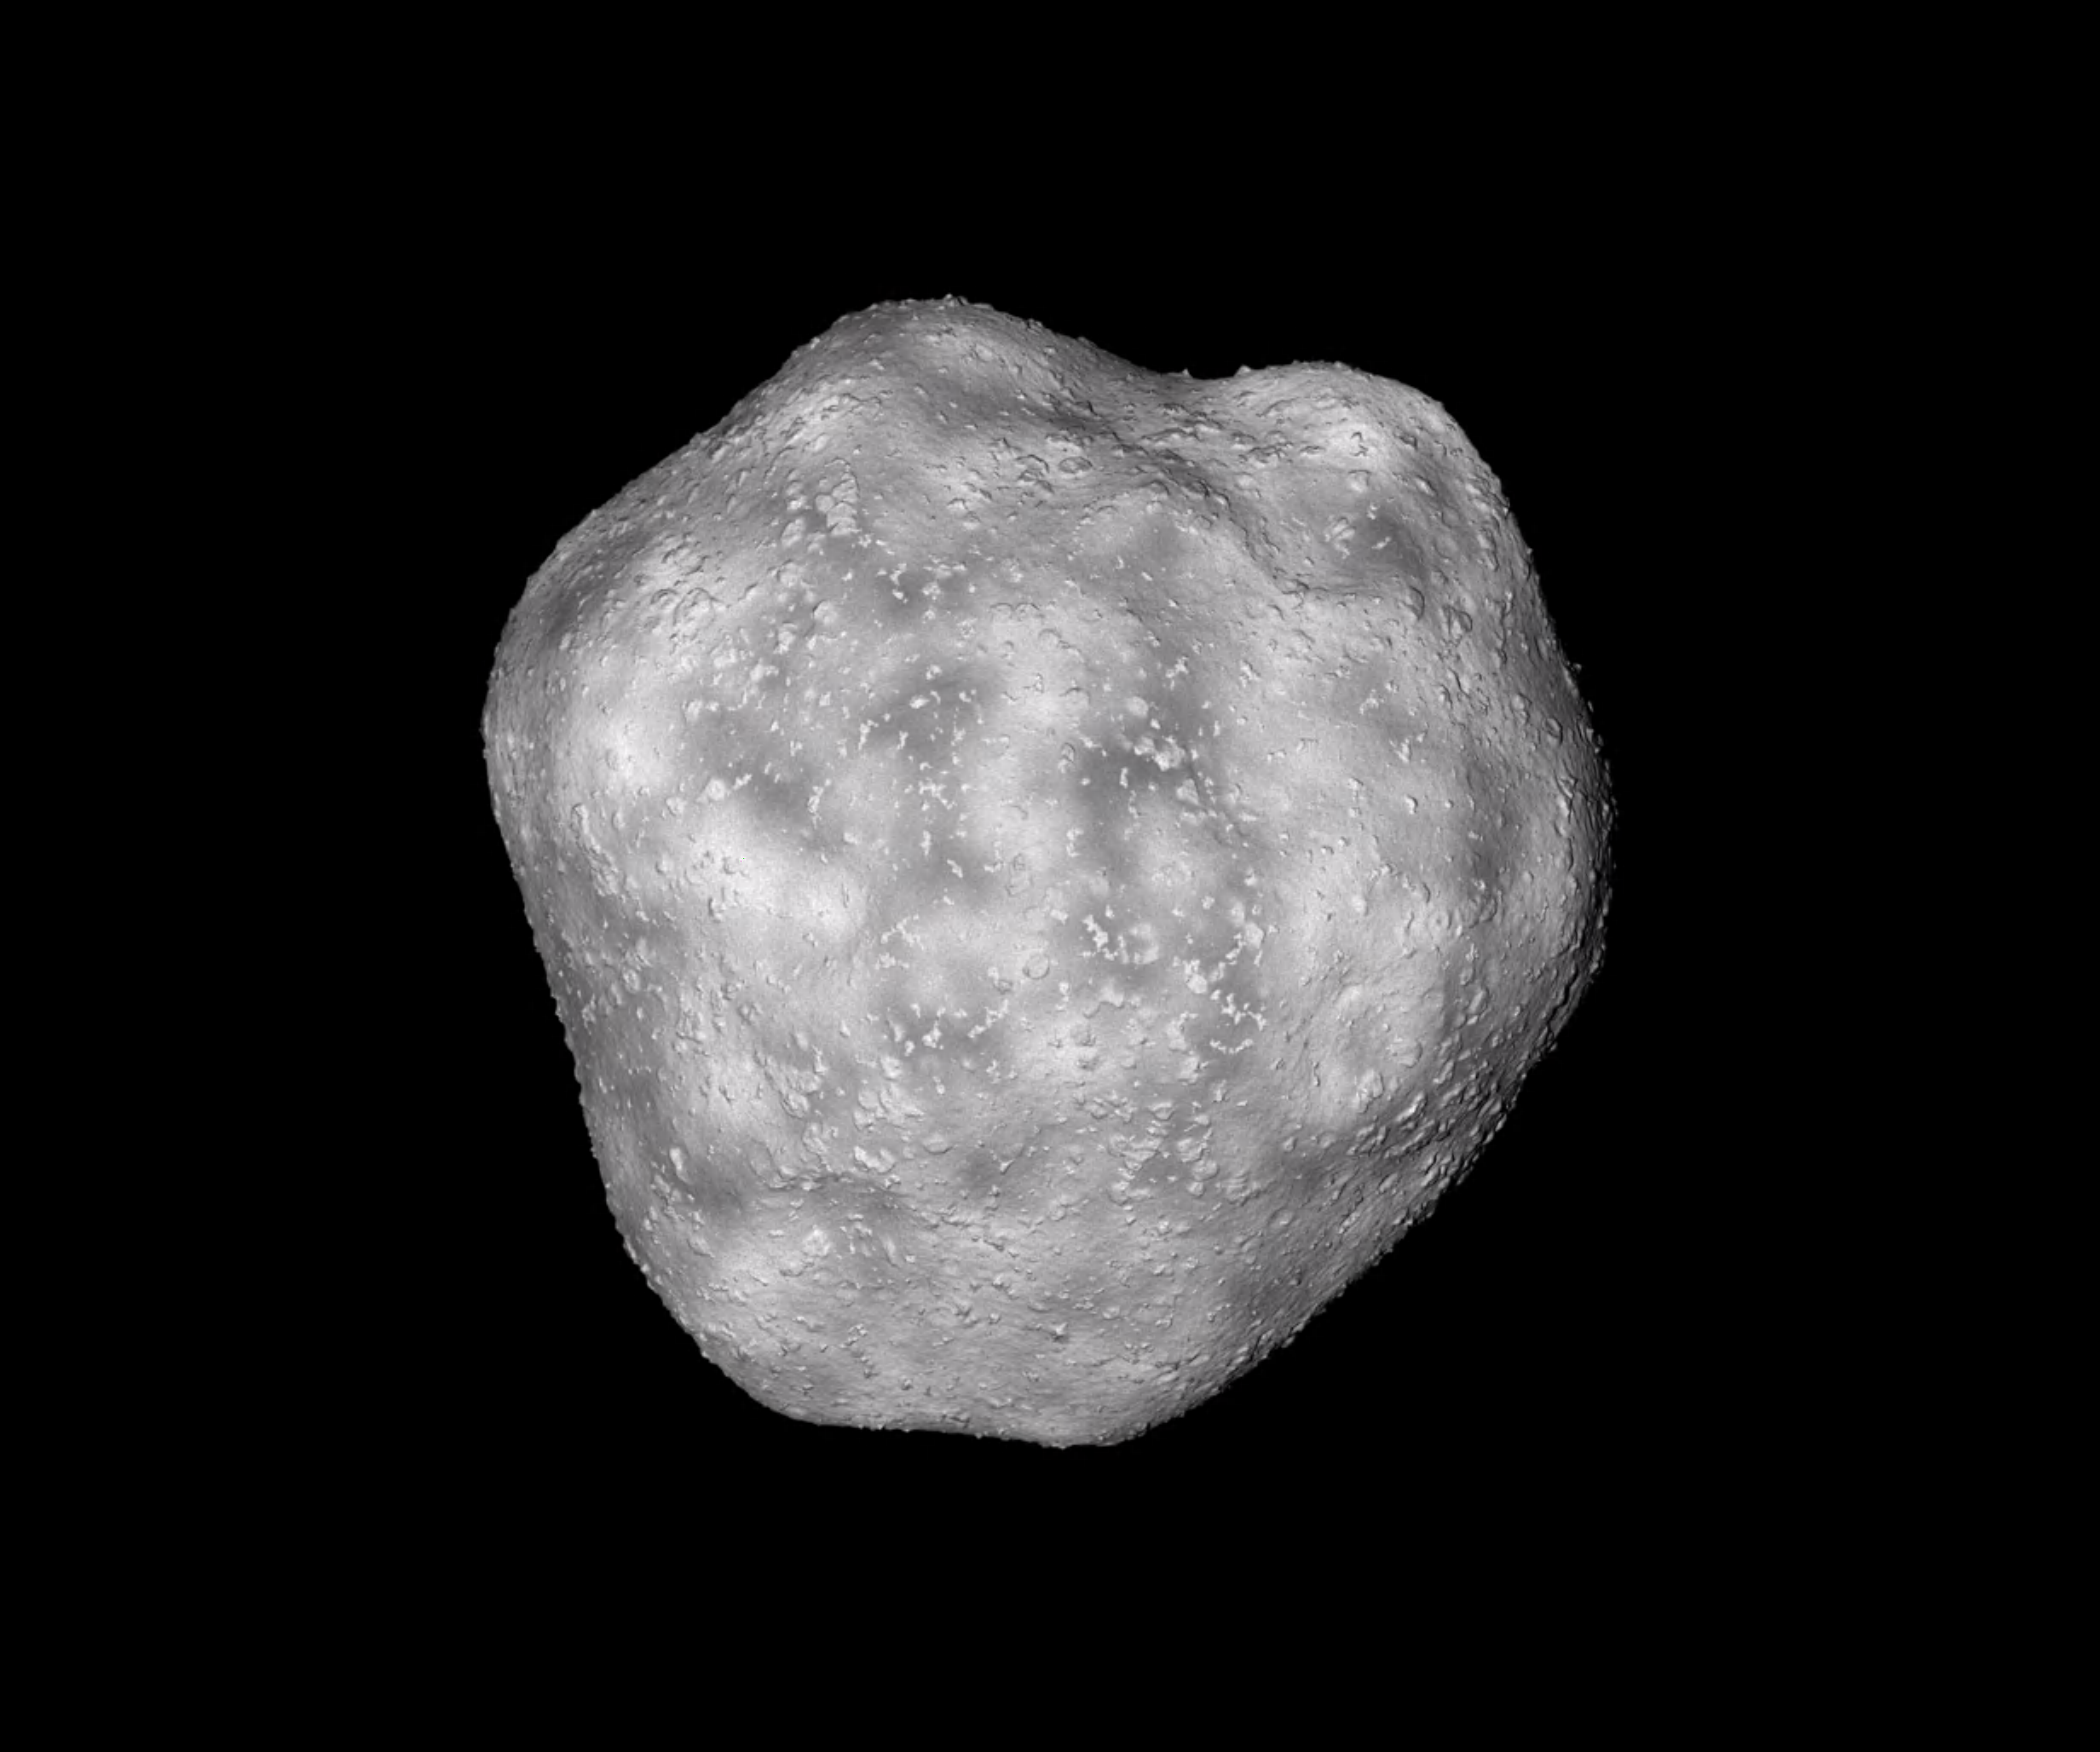
\includegraphics[width=\textwidth]{doc/thesis/0_figures/compare_quality/set1/jp2_5.png}
        \caption{}
        \label{fig:img_quality_comp_jp2_5_orig}
    \end{subfigure}
    \begin{subfigure}[b]{0.48\textwidth}
        \centering
        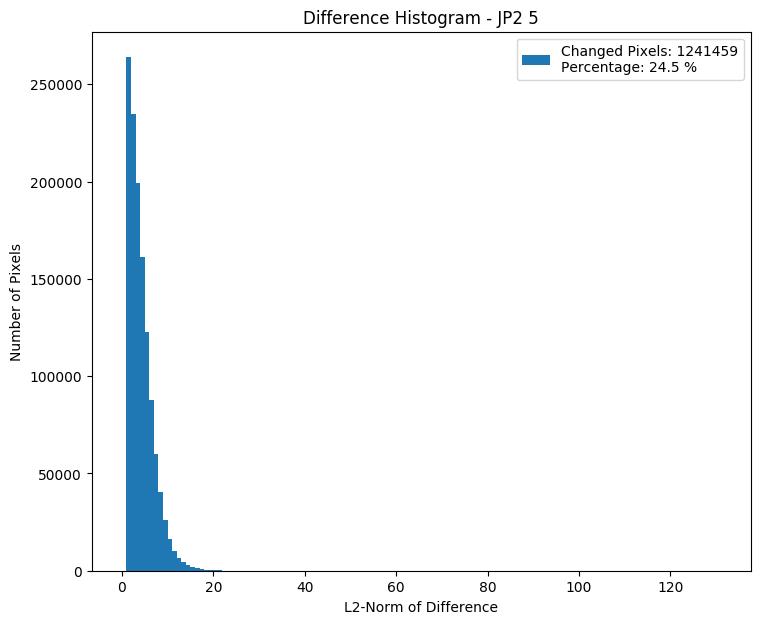
\includegraphics[width=\textwidth]{doc/thesis/0_figures/compare_quality/set1/jp2_5_diff_histogram.png}
        \caption{}
        \label{fig:img_quality_comp_jp2_5_histo}
    \end{subfigure}
    \\
    \begin{subfigure}[b]{0.48\textwidth}
        \centering
        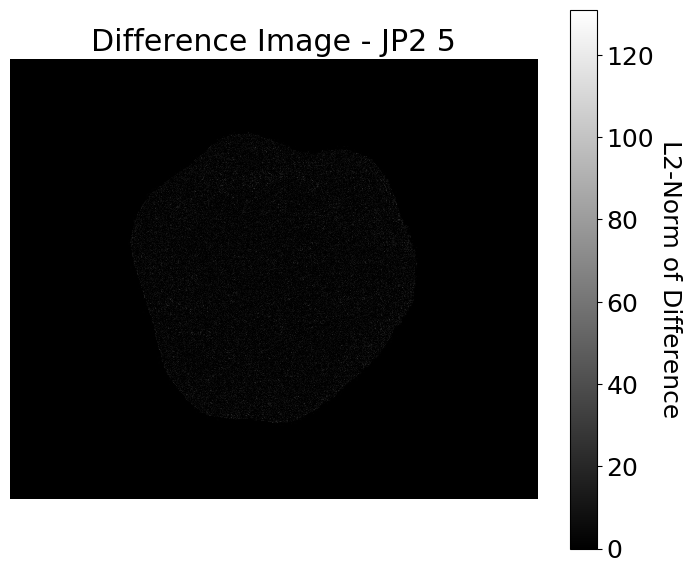
\includegraphics[width=\textwidth]{doc/thesis/0_figures/compare_quality/set1/jp2_5_diff_heatmap.png}
        \caption{}
        \label{fig:img_quality_comp_jp2_5_diff}
    \end{subfigure}
    \begin{subfigure}[b]{0.48\textwidth}
        \centering
        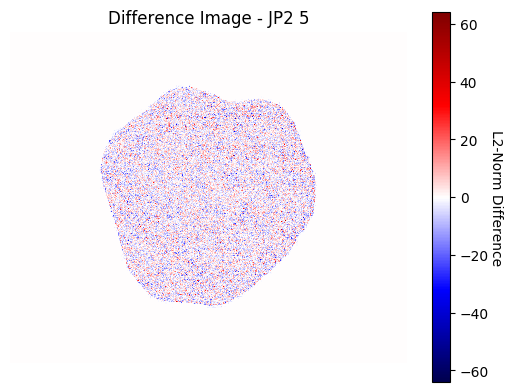
\includegraphics[width=\textwidth]{doc/thesis/0_figures/compare_quality/set1/jp2_5_diff_heatmap_rel.png}
        \caption{}
        \label{fig:img_quality_comp_jp2_5_diff_rel}
    \end{subfigure}
    \caption{Overall rendered image after compression with \gls{jp2} quality level 5. The L2-norm is applied to the difference between the greyscale images of the lossless and respective lossy image. (a) Image after lossy compression. (b) Histogram of L2-norms of differences. (c) L2-norm difference image with a colour scale from $0$ to $131$ for comparison between various compression levels. (d) L2-norm difference image with a colour scale from $0$ to the maximum L2-norm value for better visibility of compression effects.}
    \label{fig:img_quality_comp_jp2_5}
\end{figure}


\begin{figure}[htb]
    \centering
    \begin{subfigure}[b]{0.48\textwidth}
        \centering
        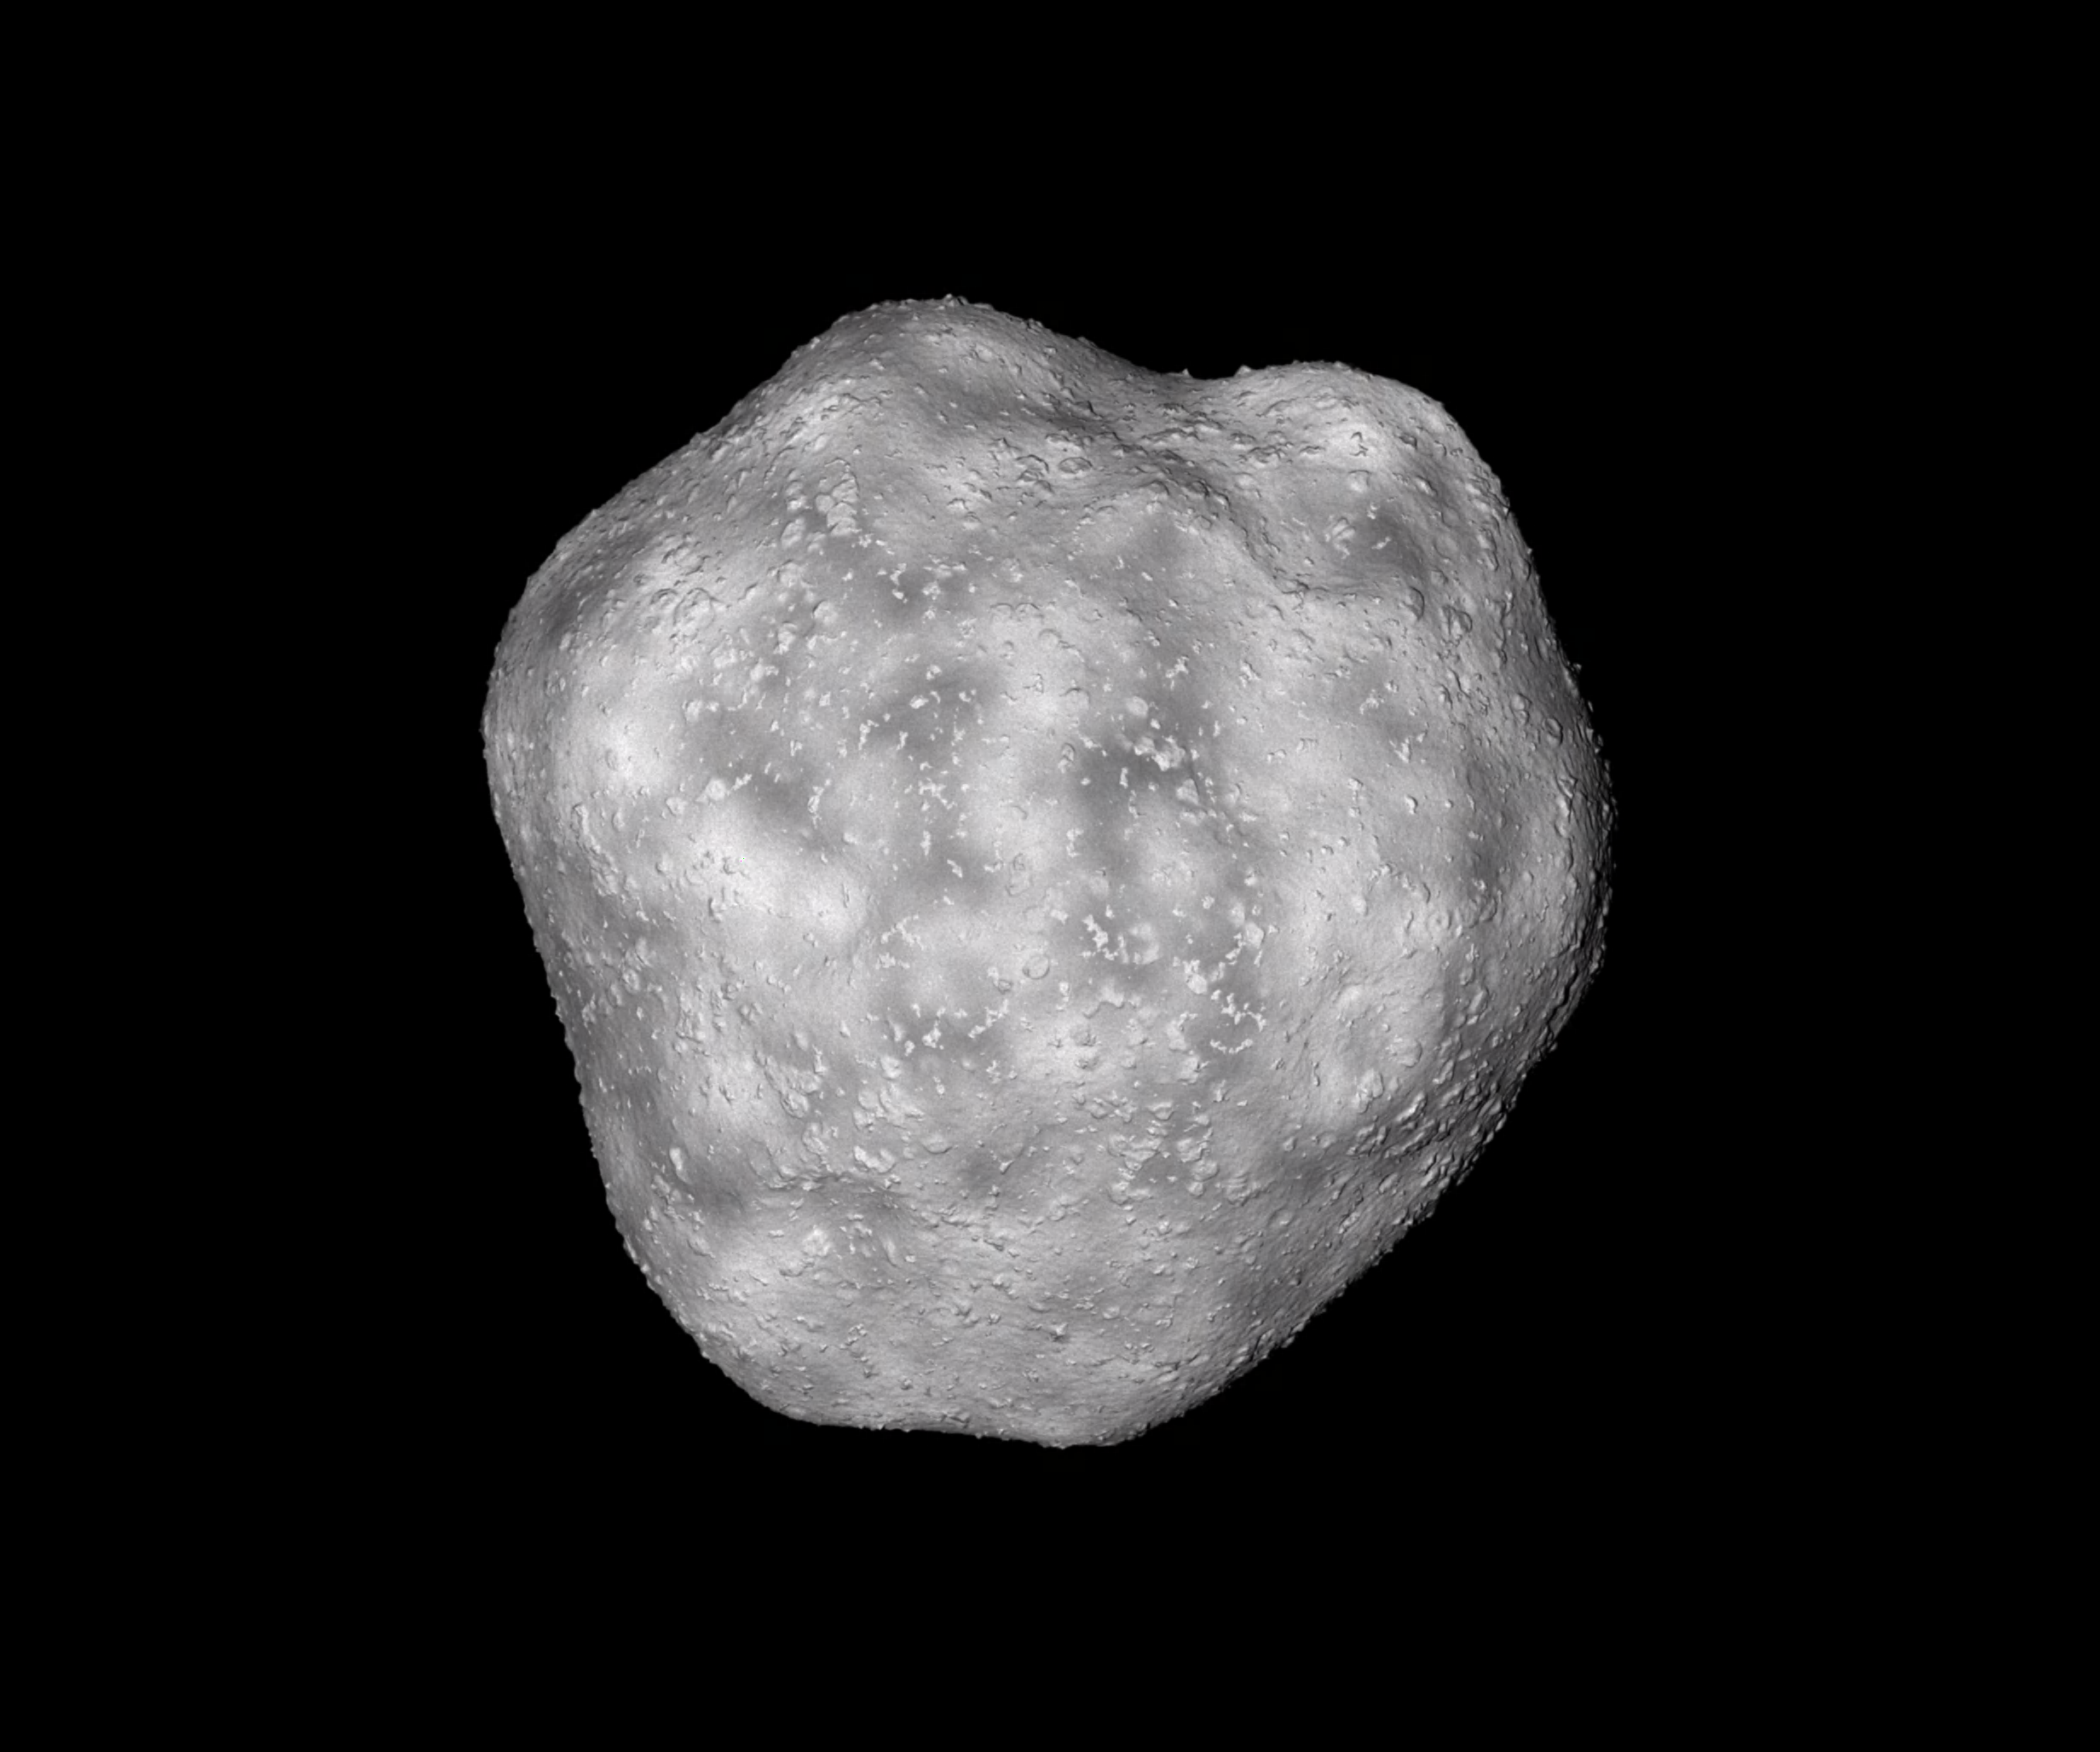
\includegraphics[width=\textwidth]{doc/thesis/0_figures/compare_quality/set1/jp2_10.png}
        \caption{}
        \label{fig:img_quality_comp_jp2_10_orig}
    \end{subfigure}
    \begin{subfigure}[b]{0.48\textwidth}
        \centering
        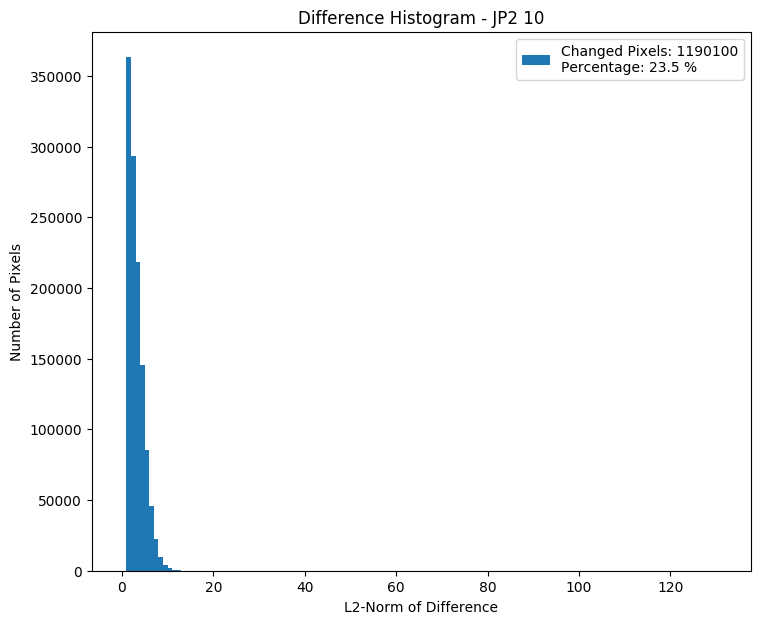
\includegraphics[width=\textwidth]{doc/thesis/0_figures/compare_quality/set1/jp2_10_diff_histogram.png}
        \caption{}
        \label{fig:img_quality_comp_jp2_10_histo}
    \end{subfigure}
    \\
    \begin{subfigure}[b]{0.48\textwidth}
        \centering
        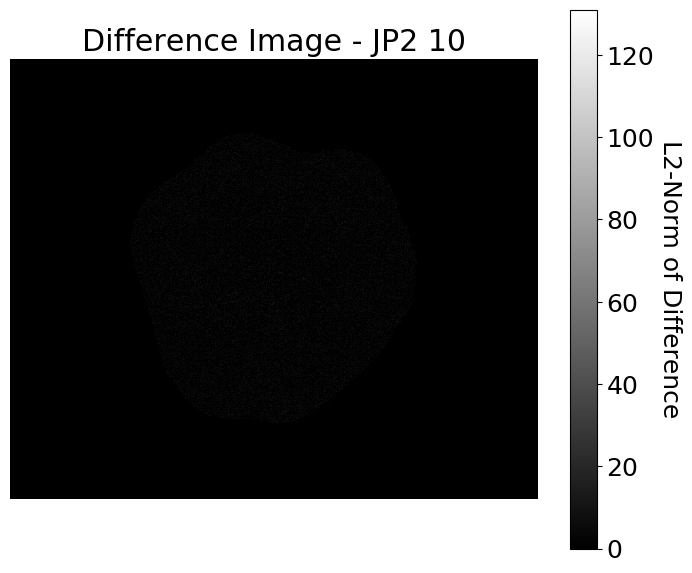
\includegraphics[width=\textwidth]{doc/thesis/0_figures/compare_quality/set1/jp2_10_diff_heatmap.png}
        \caption{}
        \label{fig:img_quality_comp_jp2_10_diff}
    \end{subfigure}
    \begin{subfigure}[b]{0.48\textwidth}
        \centering
        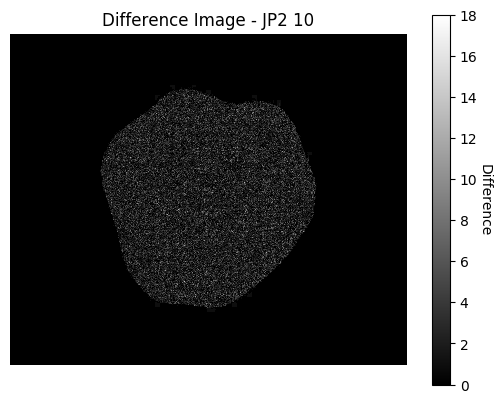
\includegraphics[width=\textwidth]{doc/thesis/0_figures/compare_quality/set1/jp2_10_diff_heatmap_rel.png}
        \caption{}
        \label{fig:img_quality_comp_jp2_10_diff_rel}
    \end{subfigure}
    \caption{Overall rendered image after compression with \gls{jp2} quality level 10. The L2-norm is applied to the difference between the greyscale images of the lossless and respective lossy image. (a) Image after lossy compression. (b) Histogram of L2-norms of differences. (c) L2-norm difference image with a colour scale from $0$ to $131$ for comparison between various compression levels. (d) L2-norm difference image with a colour scale from $0$ to the maximum L2-norm value for better visibility of compression effects.}
    \label{fig:img_quality_comp_jp2_10}
\end{figure}

\begin{figure}[htb]
    \centering
    \begin{subfigure}[b]{0.48\textwidth}
        \centering
        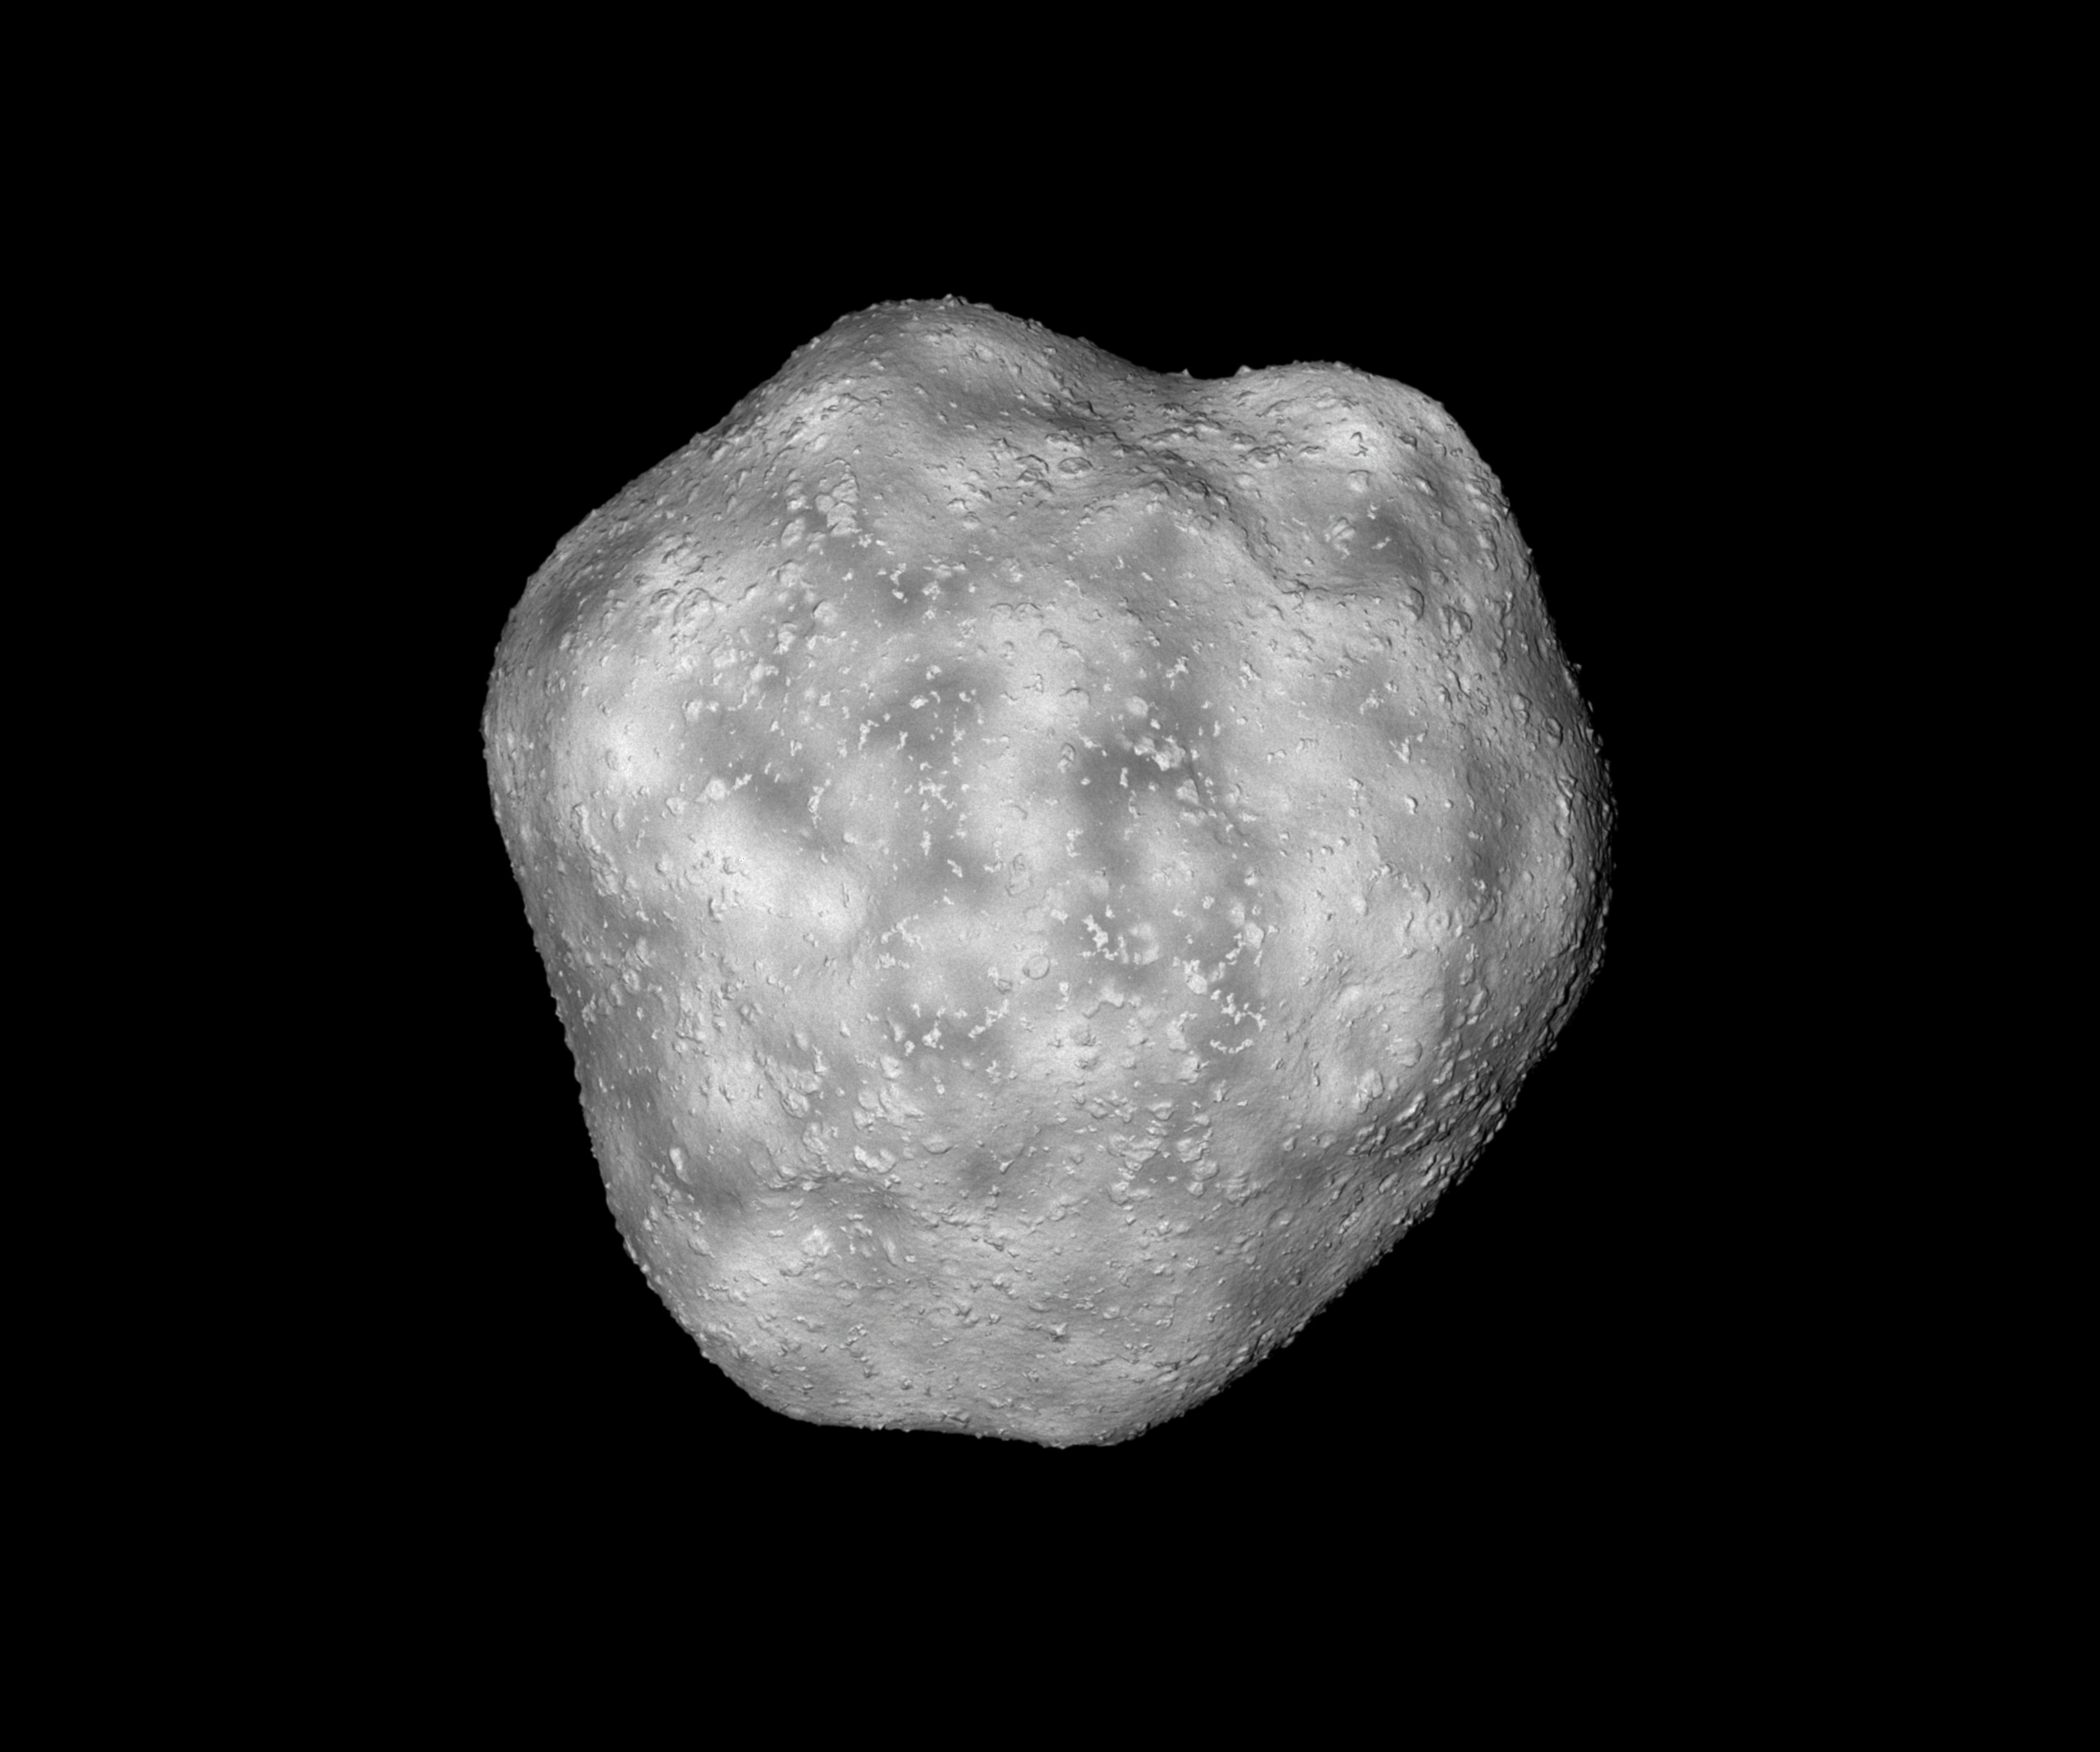
\includegraphics[width=\textwidth]{doc/thesis/0_figures/compare_quality/set1/jp2_100.png}
        \caption{}
        \label{fig:img_quality_comp_jp2_100_orig}
    \end{subfigure}
    \begin{subfigure}[b]{0.48\textwidth}
        \centering
        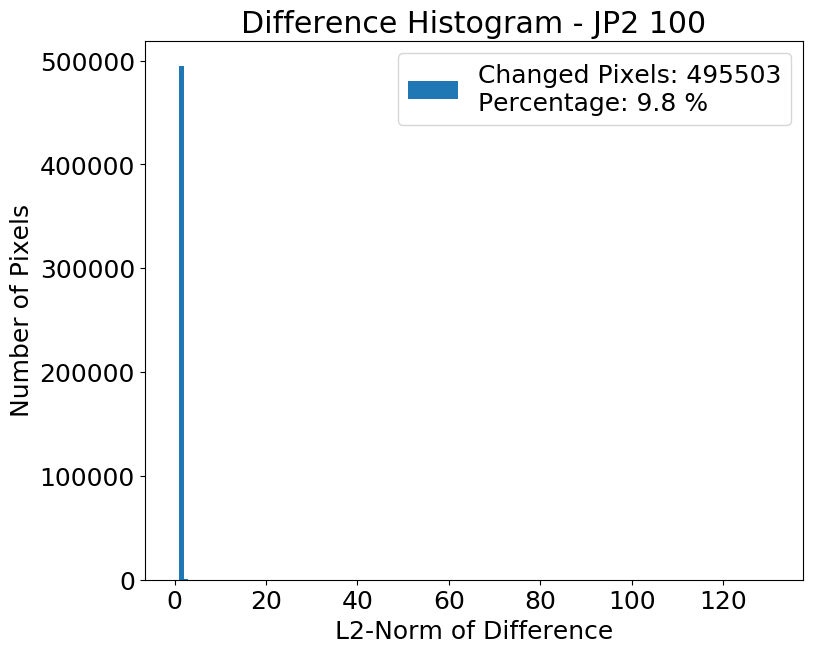
\includegraphics[width=\textwidth]{doc/thesis/0_figures/compare_quality/set1/jp2_100_diff_histogram.png}
        \caption{}
        \label{fig:img_quality_comp_jp2_100_histo}
    \end{subfigure}
    \\
    \begin{subfigure}[b]{0.48\textwidth}
        \centering
        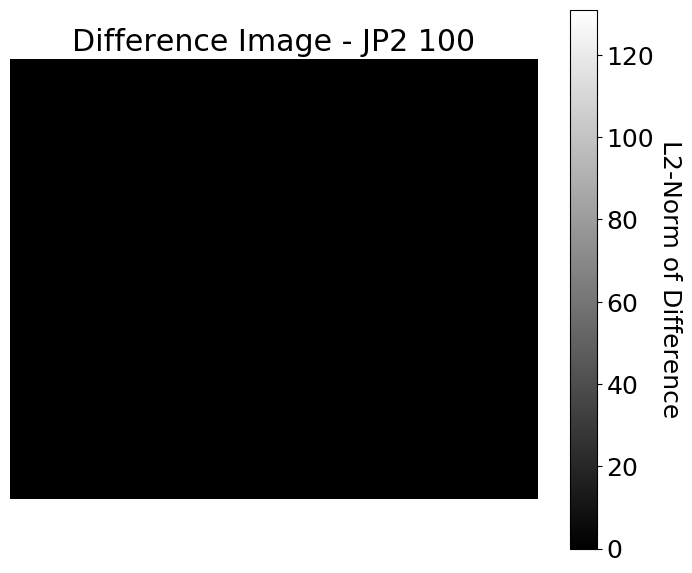
\includegraphics[width=\textwidth]{doc/thesis/0_figures/compare_quality/set1/jp2_100_diff_heatmap.png}
        \caption{}
        \label{fig:img_quality_comp_jp2_100_diff}
    \end{subfigure}
    \begin{subfigure}[b]{0.48\textwidth}
        \centering
        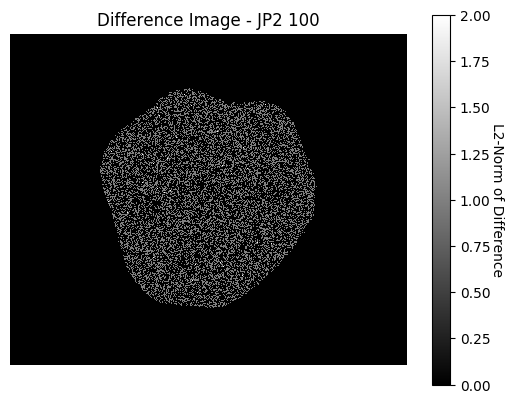
\includegraphics[width=\textwidth]{doc/thesis/0_figures/compare_quality/set1/jp2_100_diff_heatmap_rel.png}
        \caption{}
        \label{fig:img_quality_comp_jp2_100_diff_rel}
    \end{subfigure}
    \caption{Overall rendered image after compression with \gls{jp2} quality level 100. The L2-norm is applied to the difference between the greyscale images of the lossless and respective lossy image. (a) Image after lossy compression. (b) Histogram of L2-norms of differences. (c) L2-norm difference image with a colour scale from $0$ to $131$ for comparison between various compression levels. (d) L2-norm difference image with a colour scale from $0$ to the maximum L2-norm value for better visibility of compression effects.}
    \label{fig:img_quality_comp_jp2_100}
\end{figure}

\begin{figure}[htb]
    \centering
    \begin{subfigure}[b]{0.48\textwidth}
        \centering
        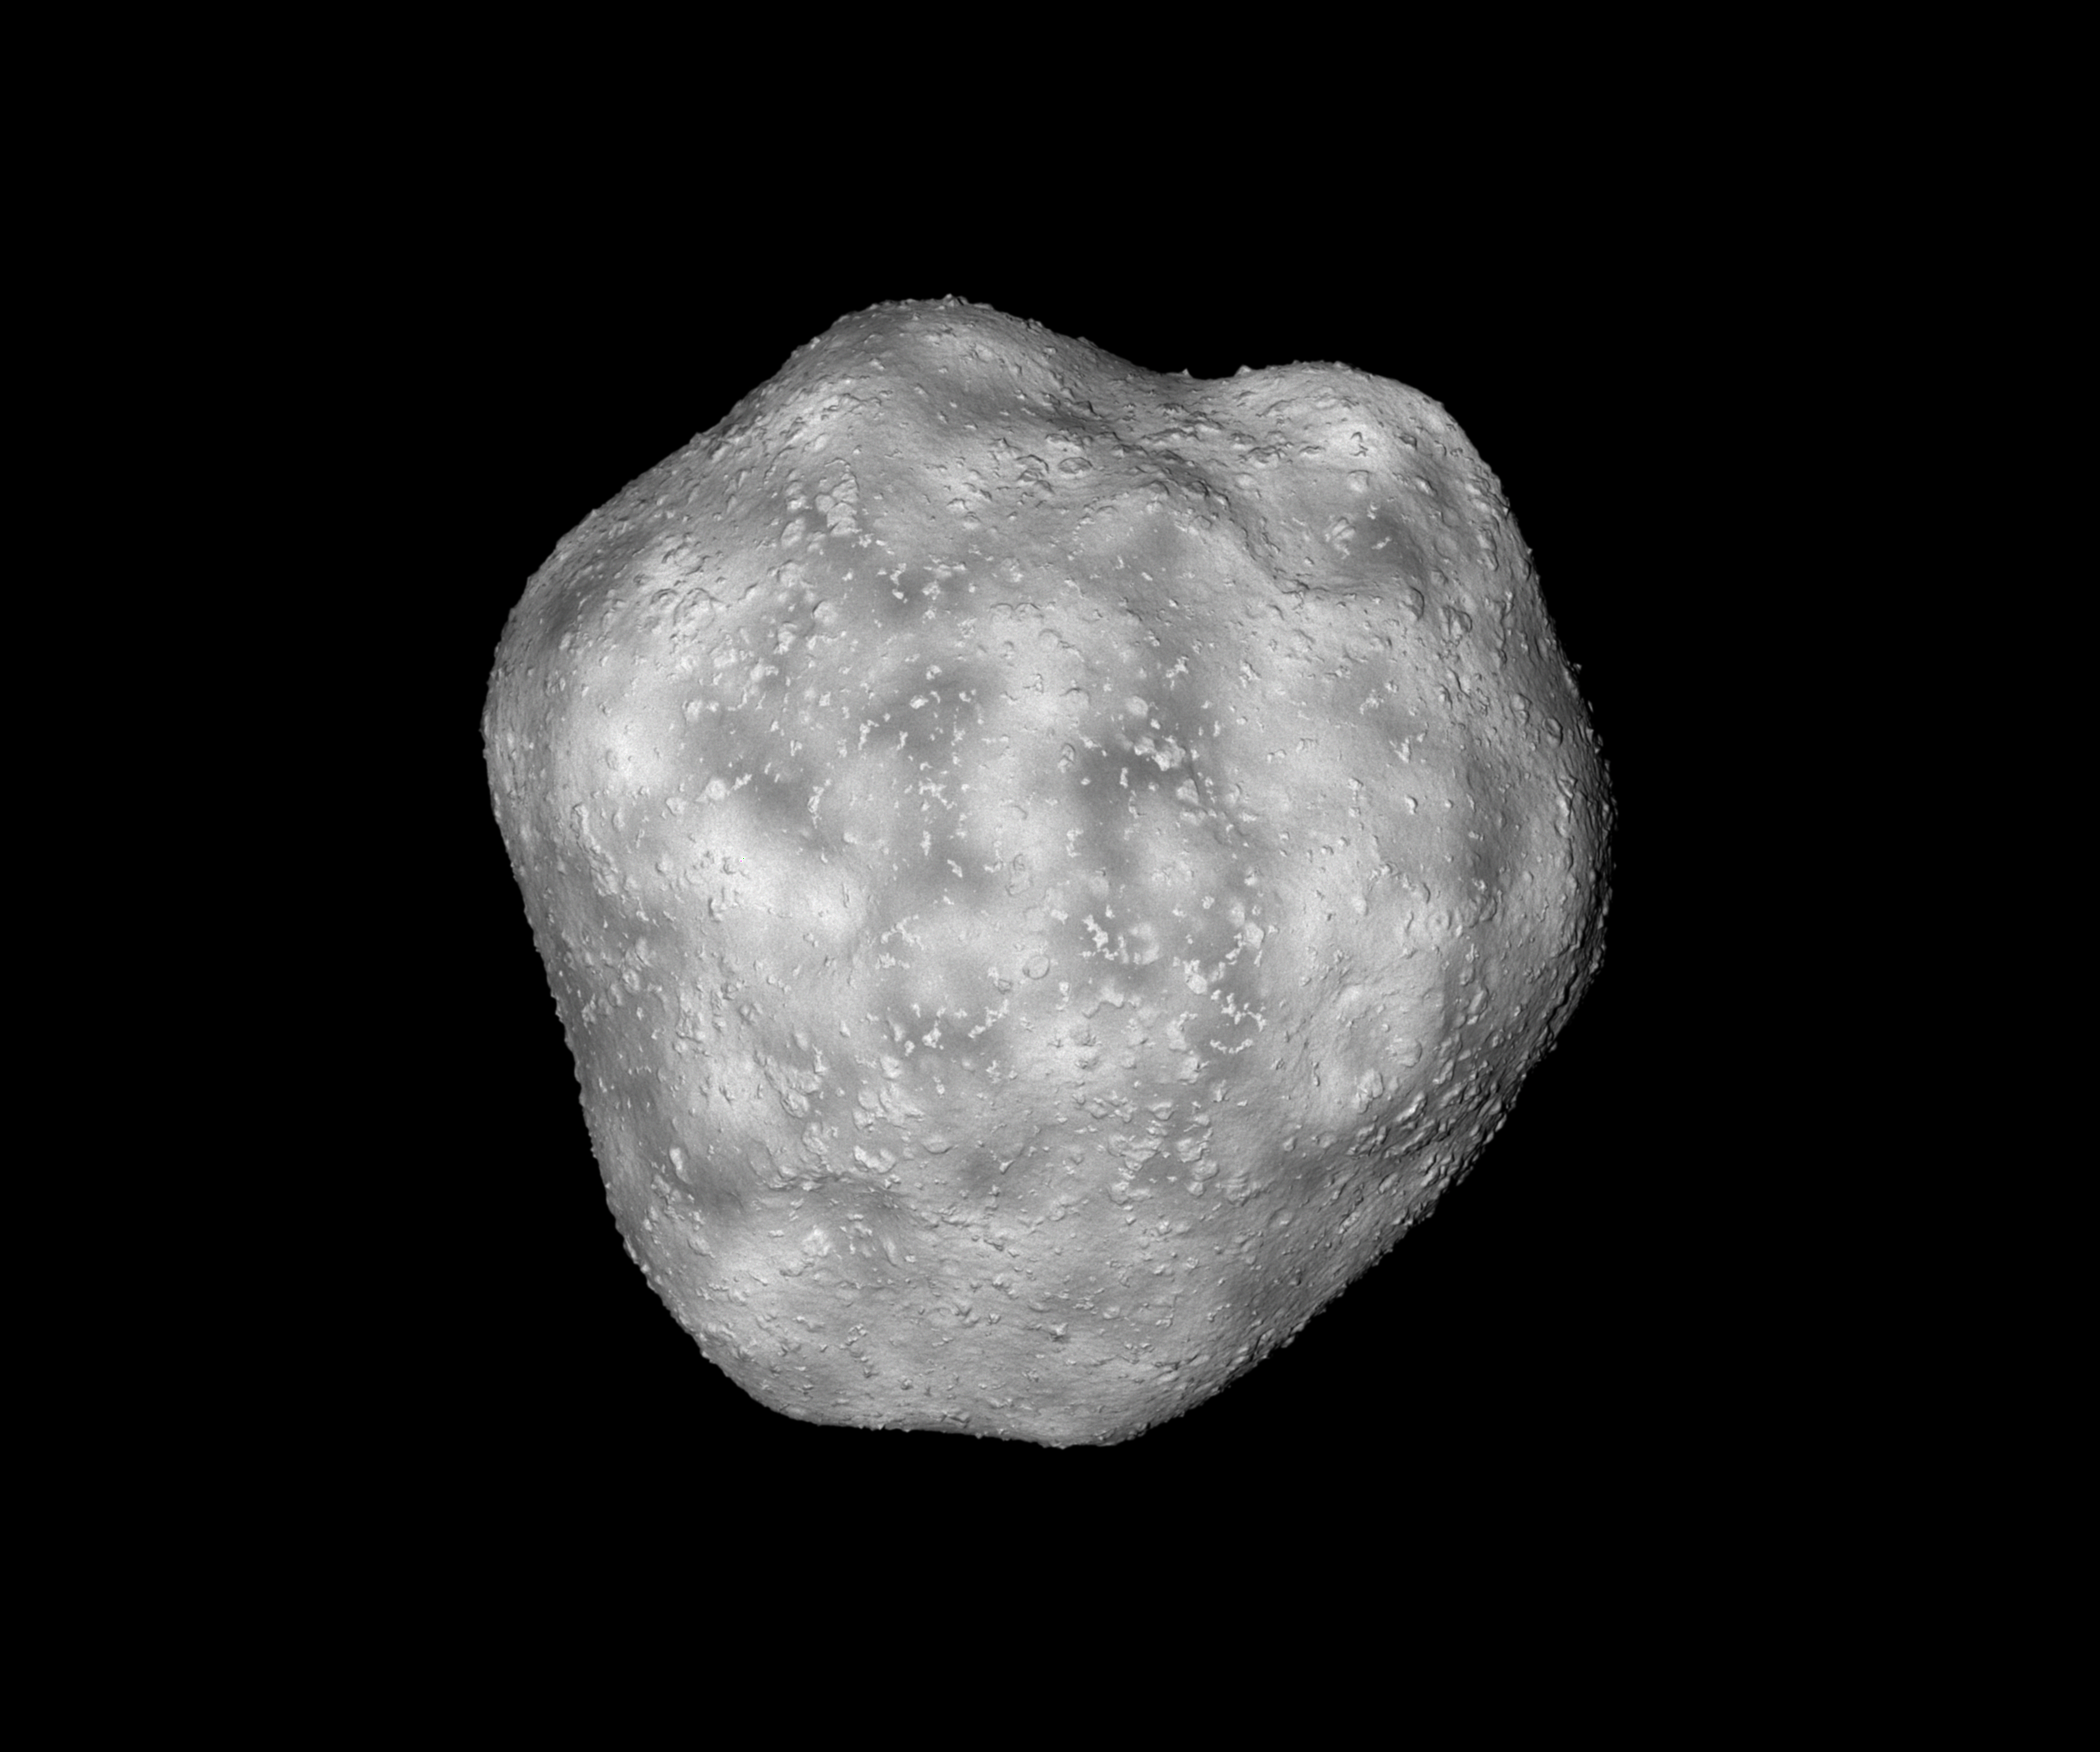
\includegraphics[width=\textwidth]{doc/thesis/0_figures/compare_quality/set1/jp2_1000.png}
        \caption{}
        \label{fig:img_quality_comp_jp2_1000_orig}
    \end{subfigure}
    \begin{subfigure}[b]{0.48\textwidth}
        \centering
        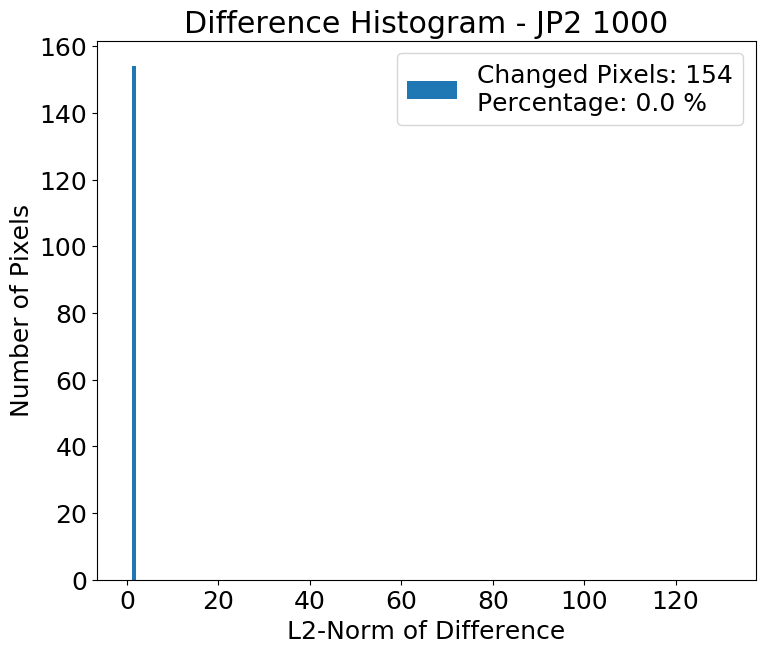
\includegraphics[width=\textwidth]{doc/thesis/0_figures/compare_quality/set1/jp2_1000_diff_histogram.png}
        \caption{}
        \label{fig:img_quality_comp_jp2_1000_histo}
    \end{subfigure}
    \\
    \begin{subfigure}[b]{0.48\textwidth}
        \centering
        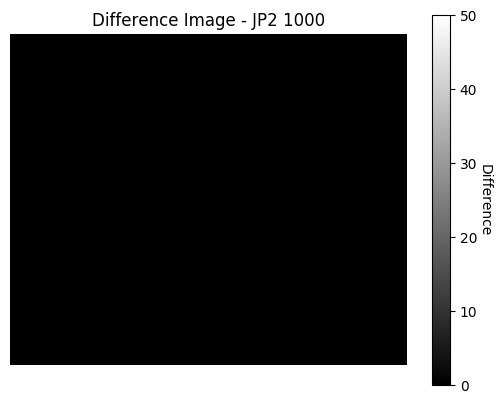
\includegraphics[width=\textwidth]{doc/thesis/0_figures/compare_quality/set1/jp2_1000_diff_heatmap.png}
        \caption{}
        \label{fig:img_quality_comp_jp2_1000_diff}
    \end{subfigure}
    \begin{subfigure}[b]{0.48\textwidth}
        \centering
        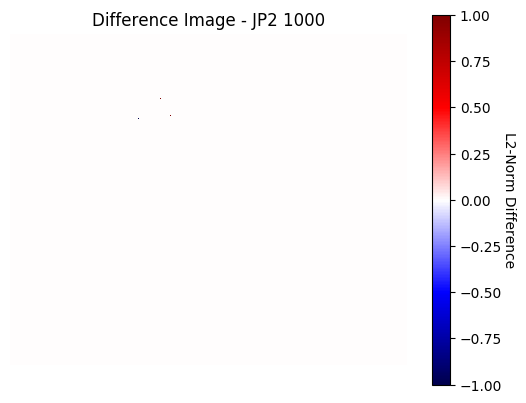
\includegraphics[width=\textwidth]{doc/thesis/0_figures/compare_quality/set1/jp2_1000_diff_heatmap_rel.png}
        \caption{}
        \label{fig:img_quality_comp_jp2_1000_diff_rel}
    \end{subfigure}
    \caption{Overall rendered image after compression with \gls{jp2} quality level 1000. The L2-norm is applied to the difference between the greyscale images of the lossless and respective lossy image. (a) Image after lossy compression. (b) Histogram of L2-norms of differences. (c) L2-norm difference image with a colour scale from $0$ to $131$ for comparison between various compression levels. (d) L2-norm difference image with a colour scale from $0$ to the maximum L2-norm value for better visibility of compression effects.}
    \label{fig:img_quality_comp_jp2_1000}
\end{figure}

Overall images show that lossy compression introduces artefacts for all quality levels. Visual inspection of the rendered images does not reveal many changes between different quality levels. However, the histograms reveal that the number of altered pixels and the amount of alteration increases with decreasing quality level. The difference image for quality level 1000 in Figure~\ref{fig:img_quality_comp_jp2_1000_diff_rel} shows the minute changes from compression. The difference images in Figures~\ref{fig:img_quality_comp_jp2_1_diff_rel}, Figure~\ref{fig:img_quality_comp_jp2_5_diff_rel}, Figure~\ref{fig:img_quality_comp_jp2_10_diff_rel} and Figure~\ref{fig:img_quality_comp_jp2_100_diff_rel} outline the shape of the \gls{sssb} showing that compression artefacts are spread across the entire \gls{sssb}. However, when comparing the difference images in Figures~\ref{fig:img_quality_comp_jp2_1_diff}, \ref{fig:img_quality_comp_jp2_5_diff}, \ref{fig:img_quality_comp_jp2_10_diff}, \ref{fig:img_quality_comp_jp2_100_diff} and \ref{fig:img_quality_comp_jp2_1000_diff} which use the same scale for all quality levels, we see the alteration in quality levels \SI{100}{} and \SI{1000}{} are much lower compared to quality levels \SI{1}{}, \SI{5}{} and \SI{10}{}.

Figures~\ref{fig:img_quality_comp_jp2_1_center} to \ref{fig:img_quality_comp_jp2_1000_center} show the compressed closeup image, the difference histograms as well as the difference images after compression with \gls{jp2} with quality levels \SI{1}{}, \SI{5}{}, \SI{10}{}, \SI{100}{} and \SI{1000}{}.

\begin{figure}[htb]
    \centering
    \begin{subfigure}[b]{0.48\textwidth}
        \centering
        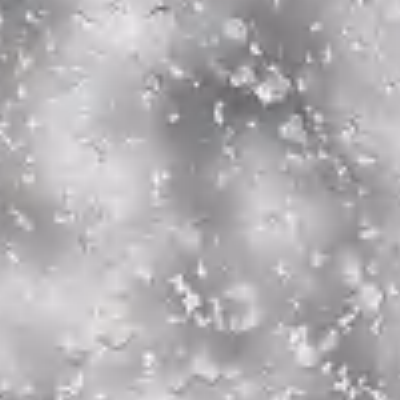
\includegraphics[width=\textwidth]{doc/thesis/0_figures/compare_quality/set1/jp2_1_center.png}
        \caption{}
        \label{fig:img_quality_comp_jp2_1_center_orig}
    \end{subfigure}
    \begin{subfigure}[b]{0.48\textwidth}
        \centering
        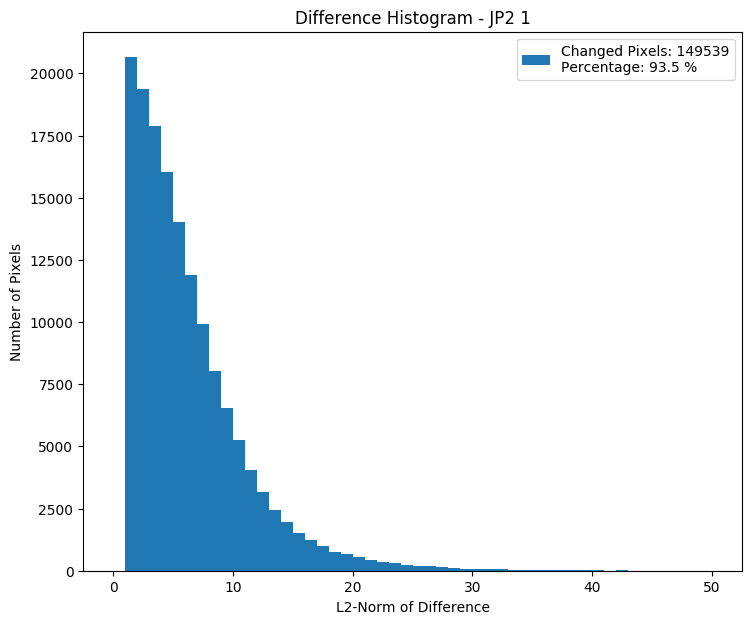
\includegraphics[width=\textwidth]{doc/thesis/0_figures/compare_quality/set1/jp2_1_center_diff_histogram.png}
        \caption{}
        \label{fig:img_quality_comp_jp2_1_center_histo}
    \end{subfigure}
    \\
    \begin{subfigure}[b]{0.48\textwidth}
        \centering
        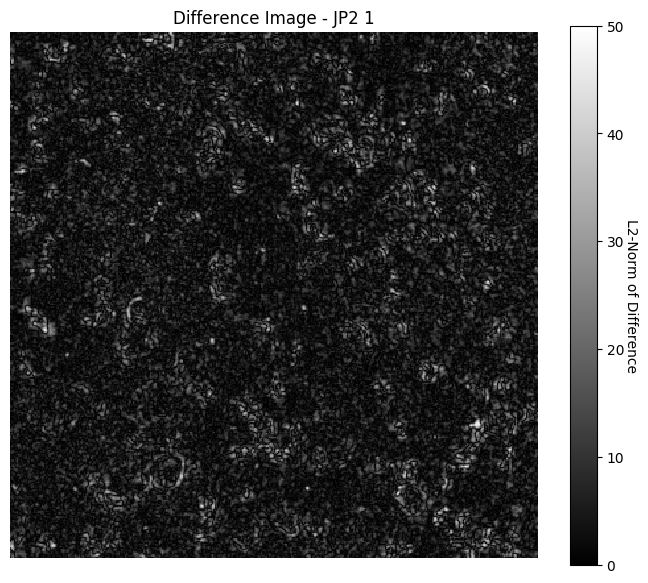
\includegraphics[width=\textwidth]{doc/thesis/0_figures/compare_quality/set1/jp2_1_center_diff_heatmap.png}
        \caption{}
        \label{fig:img_quality_comp_jp2_1_center_diff}
    \end{subfigure}
    \begin{subfigure}[b]{0.48\textwidth}
        \centering
        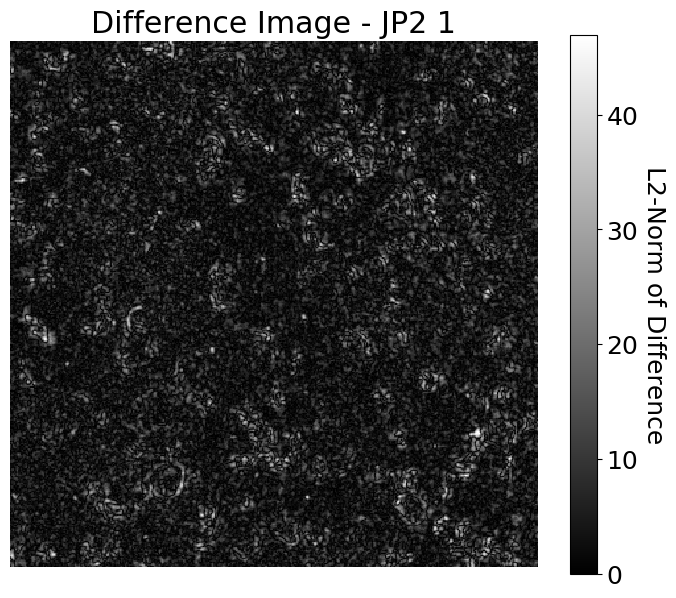
\includegraphics[width=\textwidth]{doc/thesis/0_figures/compare_quality/set1/jp2_1_center_diff_heatmap_rel.png}
        \caption{}
        \label{fig:img_quality_comp_jp2_1_center_diff_rel}
    \end{subfigure}
    \caption{Close-up rendered image after compression with \gls{jp2} quality level 1. The L2-norm is applied to the difference between the greyscale images of the lossless and respective lossy image. (a) Image after lossy compression. (b) Histogram of L2-norms of differences. (c) L2-norm difference image with a colour scale from $0$ to $131$ for comparison between various compression levels. (d) L2-norm difference image with a colour scale from $0$ to the maximum L2-norm value for better visibility of compression effects.}
    \label{fig:img_quality_comp_jp2_1_center}
\end{figure}

\begin{figure}[htb]
    \centering
    \begin{subfigure}[b]{0.48\textwidth}
        \centering
        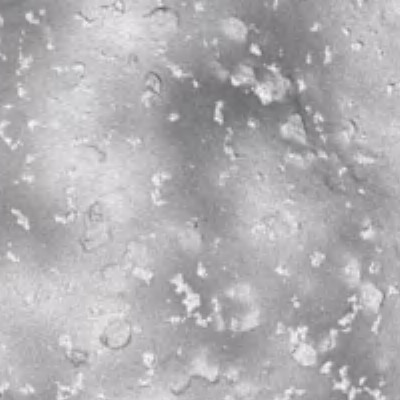
\includegraphics[width=\textwidth]{doc/thesis/0_figures/compare_quality/set1/jp2_5_center.png}
        \caption{}
        \label{fig:img_quality_comp_jp2_5_center_orig}
    \end{subfigure}
    \begin{subfigure}[b]{0.48\textwidth}
        \centering
        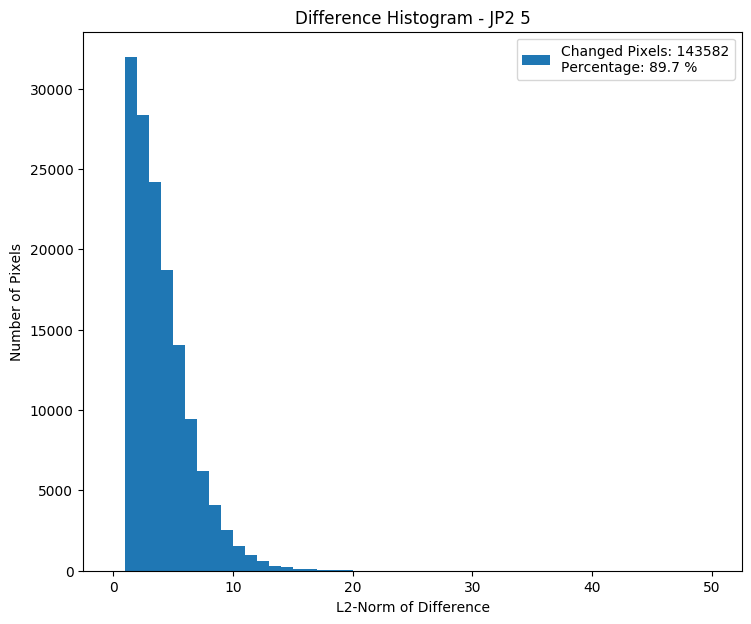
\includegraphics[width=\textwidth]{doc/thesis/0_figures/compare_quality/set1/jp2_5_center_diff_histogram.png}
        \caption{}
        \label{fig:img_quality_comp_jp2_5_center_histo}
    \end{subfigure}
    \\
    \begin{subfigure}[b]{0.48\textwidth}
        \centering
        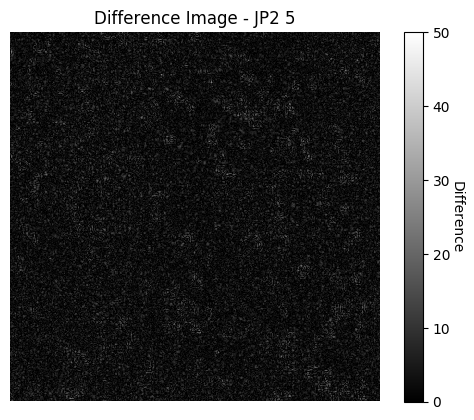
\includegraphics[width=\textwidth]{doc/thesis/0_figures/compare_quality/set1/jp2_5_center_diff_heatmap.png}
        \caption{}
        \label{fig:img_quality_comp_jp2_5_center_diff}
    \end{subfigure}
    \begin{subfigure}[b]{0.48\textwidth}
        \centering
        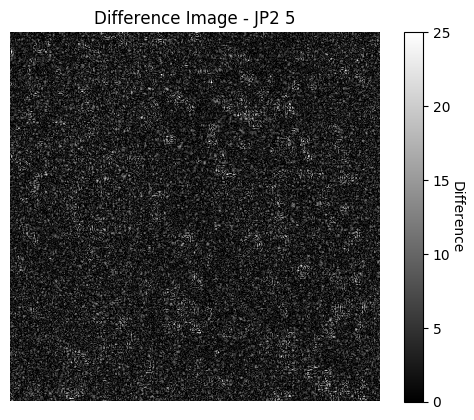
\includegraphics[width=\textwidth]{doc/thesis/0_figures/compare_quality/set1/jp2_5_center_diff_heatmap_rel.png}
        \caption{}
        \label{fig:img_quality_comp_jp2_5_center_diff_rel}
    \end{subfigure}
    \caption{Close-up rendered image after compression with \gls{jp2} quality level 5. The L2-norm is applied to the difference between the greyscale images of the lossless and respective lossy image. (a) Image after lossy compression. (b) Histogram of L2-norms of differences. (c) L2-norm difference image with a colour scale from $0$ to $131$ for comparison between various compression levels. (d) L2-norm difference image with a colour scale from $0$ to the maximum L2-norm value for better visibility of compression effects.}
    \label{fig:img_quality_comp_jp2_5_center}
\end{figure}

\begin{figure}[htb]
    \centering
    \begin{subfigure}[b]{0.48\textwidth}
        \centering
        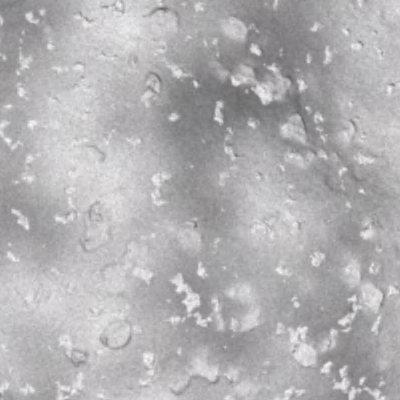
\includegraphics[width=\textwidth]{doc/thesis/0_figures/compare_quality/set1/jp2_10_center.png}
        \caption{}
        \label{fig:img_quality_comp_jp2_10_center_orig}
    \end{subfigure}
    \begin{subfigure}[b]{0.48\textwidth}
        \centering
        \includegraphics[width=\textwidth]{doc/thesis/0_figures/compare_quality/set1/jp2_10_center_diff_histogram.png}
        \caption{}
        \label{fig:img_quality_comp_jp2_10_center_histo}
    \end{subfigure}
    \\
    \begin{subfigure}[b]{0.48\textwidth}
        \centering
        \includegraphics[width=\textwidth]{doc/thesis/0_figures/compare_quality/set1/jp2_10_center_diff_heatmap.png}
        \caption{}
        \label{fig:img_quality_comp_jp2_10_center_diff}
    \end{subfigure}
    \begin{subfigure}[b]{0.48\textwidth}
        \centering
        \includegraphics[width=\textwidth]{doc/thesis/0_figures/compare_quality/set1/jp2_10_center_diff_heatmap_rel.png}
        \caption{}
        \label{fig:img_quality_comp_jp2_10_center_diff_rel}
    \end{subfigure}
    \caption{Close-up rendered image after compression with \gls{jp2} quality level 10. The L2-norm is applied to the difference between the greyscale images of the lossless and respective lossy image. (a) Image after lossy compression. (b) Histogram of L2-norms of differences. (c) L2-norm difference image with a colour scale from $0$ to $131$ for comparison between various compression levels. (d) L2-norm difference image with a colour scale from $0$ to the maximum L2-norm value for better visibility of compression effects.}
    \label{fig:img_quality_comp_jp2_10_center}
\end{figure}

\begin{figure}[htb]
    \centering
    \begin{subfigure}[b]{0.48\textwidth}
        \centering
        \includegraphics[width=\textwidth]{doc/thesis/0_figures/compare_quality/set1/jp2_100_center.png}
        \caption{}
        \label{fig:img_quality_comp_jp2_100_center_orig}
    \end{subfigure}
    \begin{subfigure}[b]{0.48\textwidth}
        \centering
        \includegraphics[width=\textwidth]{doc/thesis/0_figures/compare_quality/set1/jp2_100_center_diff_histogram.png}
        \caption{}
        \label{fig:img_quality_comp_jp2_100_center_histo}
    \end{subfigure}
    \\
    \begin{subfigure}[b]{0.48\textwidth}
        \centering
        \includegraphics[width=\textwidth]{doc/thesis/0_figures/compare_quality/set1/jp2_100_center_diff_heatmap.png}
        \caption{}
        \label{fig:img_quality_comp_jp2_100_center_diff}
    \end{subfigure}
    \begin{subfigure}[b]{0.48\textwidth}
        \centering
        \includegraphics[width=\textwidth]{doc/thesis/0_figures/compare_quality/set1/jp2_100_center_diff_heatmap_rel.png}
        \caption{}
        \label{fig:img_quality_comp_jp2_100_center_diff_rel}
    \end{subfigure}
    \caption{Close-up rendered image after compression with \gls{jp2} quality level 100. The L2-norm is applied to the difference between the greyscale images of the lossless and respective lossy image. (a) Image after lossy compression. (b) Histogram of L2-norms of differences. (c) L2-norm difference image with a colour scale from $0$ to $131$ for comparison between various compression levels. (d) L2-norm difference image with a colour scale from $0$ to the maximum L2-norm value for better visibility of compression effects.}
    \label{fig:img_quality_comp_jp2_100_center}
\end{figure}

\begin{figure}[htb]
    \centering
    \begin{subfigure}[b]{0.48\textwidth}
        \centering
        \includegraphics[width=\textwidth]{doc/thesis/0_figures/compare_quality/set1/jp2_1000_center.png}
        \caption{}
        \label{fig:img_quality_comp_jp2_1000_center_orig}
    \end{subfigure}
    \begin{subfigure}[b]{0.48\textwidth}
        \centering
        \includegraphics[width=\textwidth]{doc/thesis/0_figures/compare_quality/set1/jp2_1000_center_diff_histogram.png}
        \caption{}
        \label{fig:img_quality_comp_jp2_1000_center_histo}
    \end{subfigure}
    \\
    \begin{subfigure}[b]{0.48\textwidth}
        \centering
        \includegraphics[width=\textwidth]{doc/thesis/0_figures/compare_quality/set1/jp2_1000_center_diff_heatmap.png}
        \caption{}
        \label{fig:img_quality_comp_jp2_1000_center_diff}
    \end{subfigure}
    \begin{subfigure}[b]{0.48\textwidth}
        \centering
        \includegraphics[width=\textwidth]{doc/thesis/0_figures/compare_quality/set1/jp2_1000_center_diff_heatmap_rel.png}
        \caption{}
        \label{fig:img_quality_comp_jp2_1000_center_diff_rel}
    \end{subfigure}
    \caption{Close-up rendered image after compression with \gls{jp2} quality level 1000. The L2-norm is applied to the difference between the greyscale images of the lossless and respective lossy image. (a) Image after lossy compression. (b) Histogram of L2-norms of differences. (c) L2-norm difference image with a colour scale from $0$ to $131$ for comparison between various compression levels. (d) L2-norm difference image with a colour scale from $0$ to the maximum L2-norm value for better visibility of compression effects.}
    \label{fig:img_quality_comp_jp2_1000_center}
\end{figure}

Comparing the closeup images for the various quality levels in Figures~\ref{fig:img_quality_comp_jp2_1_center_orig}, \ref{fig:img_quality_comp_jp2_5_center_orig}, \ref{fig:img_quality_comp_jp2_10_center_orig}, \ref{fig:img_quality_comp_jp2_100_center_orig} and \ref{fig:img_quality_comp_jp2_1000_center_orig} reveals a degradation of image quality with decreasing compression quality levels. The histograms confirm that the number of altered pixels and the amount of alteration increases with decreasing quality level. The difference image for quality level 1000 in Figure~\ref{fig:img_quality_comp_jp2_1000_center_diff_rel} and the respective histogram show that there were no altered pixels for quality level 1000, i.e. the compression was lossless. The difference image in Figure~\ref{fig:img_quality_comp_jp2_100_center_diff_rel} resembles random noise. In contrast, the difference images in Figure~\ref{fig:img_quality_comp_jp2_1_center_diff_rel}, Figure~\ref{fig:img_quality_comp_jp2_5_center_diff_rel} and Figure~\ref{fig:img_quality_comp_jp2_10_center_diff_rel} show non-random artefacts related to surface features when comparing to the unaltered image in Figure~\ref{fig:img_quality_comp_jp2_1000_center_orig}. However, when comparing the difference images in Figures~\ref{fig:img_quality_comp_jp2_1_center_diff}, \ref{fig:img_quality_comp_jp2_5_center_diff}, \ref{fig:img_quality_comp_jp2_10_center_diff}, \ref{fig:img_quality_comp_jp2_100_center_diff} and \ref{fig:img_quality_comp_jp2_1000_center_diff} which use the same scale for all quality levels, we see the alteration in quality levels \SI{100}{} and \SI{1000}{} are much lower compared to quality levels \SI{1}{}, \SI{5}{} and \SI{10}{}.

When comparing the results for the overall images with the results for the closeup we see that the overall images are less altered by compression. Since the a substantial portion of the  overall images are covered by a black background, compression does change less pixels than in the closeup images. While the overall difference images resemble random noise, the closeup images reveal a relation between surface features and compression artefacts for low quality levels.

\clearpage

\subsection{Reconstruction}
\gls{sispo} reconstructs using default parameters given in Table~\ref{tab:comp_settings}. \textit{refine\_options} is set to NONE to make \gls{sfm} algorithms more likely to converge. Camera calibration as described in Section~\ref{sec:t_cv} is not needed since in space missions, the intrinsic camera parameters can be determined with sufficient accuracy before launch and therefore the parameters do not need to be optimised anymore.

\begin{table}[htb]
    \centering
    \caption{Reconstruction Settings}
    \label{tab:comp_settings}
    \begin{tabular}{l|l}
        \textbf{Parameter Name} & \textbf{Value} \\ \hline
        export\_type       & obj   \\
        focal & 66667 \\
        cam\_model & \SI{1}{}     \\
        geo\_model & \SI{10}{\kilo\meter\per\second} \\
        num\_overlaps  & \SI{4}{} \\
        use\_prior & \SI{1}{} \\
        use\_upright & \SI{0}{} \\
        force\_compute & \SI{0}{} \\
        descriptor & SIFT \\
        d\_preset & ULTRA \\
        method & FASTCASCADEHASHINGL2 \\
        refine\_options & NONE \\
        reduce\_memory & 1
    \end{tabular}
\end{table}

\gls{sispo} is choosing which result of which reconstruction method to use based on the number of reconstructed points. Comparing the chosen algorithm with the input parameter reveals that the first incremental \gls{sfm} reconstruction performs better when the fly-by distance is smaller while the second incremental \gls{sfm} algorithms performs better with farther fly-by distances.

\subsubsection{Reconstructed Model Comparison}
\Gls{3d} models were reconstructed for most scenarios presented in Table~\ref{tab:sim_params}. When using \SI{120}{} images, reconstruction was successful in all cases except for a \SI{400}{\kilo\meter} fly-by of a \SI{1}{\kilo\meter} nucleus and the highest compression ratio. Generally the number of reconstructed points decreases with a decreasing \gls{sssb} size and an increasing closest distance, i.e. with decreasing visible size in the images.
The number of points in the densified point cloud range from approximately \SI{6e6}{} for a \SI{50}{\kilo\meter} fly-by of a \SI{10}{\kilo\meter} \gls{sssb} to approximately \SI{2e3}{} for a \SI{400}{\kilo\meter} fly-by of a \SI{1}{\kilo\meter} \gls{sssb}. Since these two scenarios represent the two boundary cases of the simulation results, these are compared in more detail. The quality of other reconstructed \gls{3d} models are in between the presented results and are therefore not analysed further.

A comparison of the point clouds of the two scenarios is shown in Figure~\ref{fig:points_dense_comp}. The large variation in points after reconstruction and densification strongly influences the \gls{3d} model quality. However, both point clouds contain outliers which are removed later in the \gls{3d} models.

\begin{figure}[htb]
    \centering
        \begin{subfigure}[b]{0.42\textwidth}
            \centering
            \includegraphics[width=\textwidth,height=6.2cm]{doc/thesis/0_figures/models_quality/50_10/120_50_10_dense2.png}
            \caption{}
            \label{fig:points_50_10}
        \end{subfigure}
        \begin{subfigure}[b]{0.42\textwidth}
            \centering
            \includegraphics[width=\textwidth,height=6.2cm]{doc/thesis/0_figures/models_quality/400_1/120_400_1_points2.png}
            \caption{}
            \label{fig:points_400_1}
        \end{subfigure}
    \caption{Images showing point clouds of two fly-by scenarios of two boundary cases with working reconstructions. (a) Point cloud with $\approx\SI{6e6}{}$ points of a \SI{10}{\kilo\meter} \gls{sssb} after a \SI{50}{\kilo\meter} fly-by. (b) Point cloud with $\approx\SI{2e3}{}$ points of a \SI{1}{\kilo\meter} \gls{sssb} after a \SI{400}{\kilo\meter} fly-by. Point cloud densification failed for this scenario, therefore the sparse point cloud is depicted.}
    \label{fig:points_dense_comp}
\end{figure}

To compare the \gls{3d} models, the meshes after refinement are used, since texturing only changes the appearance but not model quality. When comparing the \gls{3d} models in Figure~\ref{fig:models_comp}, the influence of the number of points is clearly visible. It is possible to see single vertices that make up the model in Figure~\ref{fig:models_400_1}. In contrast, the more detailed model in Figure~\ref{fig:models_50_10} represents surface features such as boulders.

\begin{figure}[htb]
    \centering
        \begin{subfigure}[b]{0.42\textwidth}
            \centering
            \includegraphics[width=\textwidth,height=6.2cm]{doc/thesis/0_figures/models_quality/50_10/120_50_10_refine2.png}
            \caption{\SI{10}{\kilo\meter} \gls{sssb} after a \SI{50}{\kilo\meter} fly-by with $\approx\SI{1e6}{}$ vertices.} %1072422
            \label{fig:models_50_10}
        \end{subfigure}
        \begin{subfigure}[b]{0.42\textwidth}
            \centering
            \includegraphics[width=\textwidth,height=6.2cm]{doc/thesis/0_figures/models_quality/400_1/120_400_1_mesh2.png}
            \caption{\SI{1}{\kilo\meter} \gls{sssb} after a \SI{400}{\kilo\meter} fly-by with $\approx\SI{700}{}$ vertices.}
            \label{fig:models_400_1}
        \end{subfigure}
    \caption{Images showing \gls{3d} models reconstructed from the point clouds shown in Figure~\ref{fig:points_dense_comp}. (a) Reconstructed mesh with $\approx\SI{1e6}{}$ vertices of a \SI{10}{\kilo\meter} \gls{sssb} after a \SI{50}{\kilo\meter} fly-by. (b) Reconstructed mesh with $\approx\SI{700}{}$ vertices of a \SI{1}{\kilo\meter} \gls{sssb} after a \SI{400}{\kilo\meter} fly-by. Mesh refinement failed in this scenario, therefore the sparse mesh is depicted.}
    \label{fig:models_comp}
\end{figure}

\subsubsection{Compression Effects on Reconstructed 3D Models}
To compare  quality of the reconstructed \gls{3d} models numerically, the number of points after densification, the number of vertices and the number of faces of the refined meshed model are compared for different levels of compression for the same simulation scenario. The number of points, vertices and faces are used because they relate to the level of detail of a \gls{3d} model. Moreover, the number of points in relation to the number of vertices can be used to analyse the amount of outliers in the point cloud since outlier points cannot be included into a meaningful \gls{3d} model. All values are normalised to the \gls{png} case to compare lossless compression against lossy compression with varying quality levels.

First we compare the theoretical raw size of an image series of \SI{120}{} images to the highest compression ratio of lossless compression with \gls{png}. An image series of \SI{120}{}~\gls{rgb} images with $\SI{2454}{} \times \SI{2054}{}$~pixels and a colour depth of \SI{1}{\byte} has a data size of $d = 120 \times 2454 \times 2054 \times 3 \times \SI{1}{\byte} = \SI{1814.6}{\mega\byte}$. The \gls{png} data sets have sizes ranging from \SI{5.2}{\mega\byte} to \SI{564.6}{\mega\byte}, i.e. \SI{0.3}{\percent} to \SI{31.1}{\percent} of the raw data size depending on the simulation scenario. The varying apparent size of the nucleus and the resulting portion with constant black values of an image can be compressed well with \gls{png}.
% 564573825 / 5172917; 1814585760

Figure~\ref{fig:recon_stats_1} and Figure~\ref{fig:recon_stats_10} compare the effects of lossless compression using \gls{png} and lossy compression using \gls{jp2}.

\begin{figure}[htb]
    \centering
        \begin{subfigure}[b]{0.49\textwidth}
            \centering
            \includegraphics[width=\textwidth]{doc/thesis/0_figures/recon/50km_1k}
            \caption{}
            \label{fig:recon_120_50_1}
        \end{subfigure}
        \begin{subfigure}[b]{0.49\textwidth}
            \centering
            \includegraphics[width=\textwidth]{doc/thesis/0_figures/recon/100km_1k}
            \caption{}
            \label{fig:recon_120_100_1}
        \end{subfigure}
        \\
        \begin{subfigure}[b]{0.49\textwidth}
            \centering
            \includegraphics[width=\textwidth]{doc/thesis/0_figures/recon/200km_1k}
            \caption{}
            \label{fig:recon_120_200_1}
        \end{subfigure}
        \begin{subfigure}[b]{0.49\textwidth}
            \centering
            \includegraphics[width=\textwidth]{doc/thesis/0_figures/recon/400km_1k}
            \caption{}
            \label{fig:recon_120_400_1}
        \end{subfigure}
    \caption{Bar graphs comparing output of reconstruction after image compression with varying quality levels for a \SI{1}{\kilo\meter} \gls{sssb} with varying fly-by distances. (a) Fly-by distance \SI{50}{\kilo\meter}. (b) Fly-by distance \SI{100}{\kilo\meter}. (c) Fly-by distance \SI{200}{\kilo\meter}. (d) Fly-by distance \SI{400}{\kilo\meter}.}
    \label{fig:recon_stats_1}
\end{figure}

Figure~\ref{fig:recon_stats_1} reveals that for a \SI{100}{\kilo\meter} fly-by, the number of reconstructed vertices and faces increases with increasing degrees of compression. The artefacts introduced by compression create additional features for the \gls{sfm} algorithms. While the number of points for the lowest quality level in Figure~\ref{fig:recon_120_50_1} contains more points than the \gls{png} case, the number of vertices and faces is much lower. Hence the densified point cloud contained a higher number of outliers that were removed during meshed creation. If the number of vertices decreased more than the number of points, compression increased the number of outliers. In contrast, in the \SI{400}{\kilo\meter} case, the compression deteriorated the quality of the reconstructed models substantially. Due to the small visual size of the \gls{sssb} nucleus, there is only a small number of usable features which are removed by compression. Only for the \SI{200}{\kilo\meter} case, the quality of the reconstructed \gls{3d} model decreases gradually with decreasing data size.

Figure~\ref{fig:recon_stats_1} shows that compression with \gls{jp2} quality levels 1000 and 100 do not differ much. For the \SI{100}{\kilo\meter} and \SI{200}{\kilo\meter} cases, even \gls{jp2} quality 10 has the same size as 100 and 1000. This can be explained with a high number of black pixels which can be compressed efficiently without losing information and a small visible nucleus size.

\begin{figure}[htb]
    \centering
        \begin{subfigure}[b]{0.49\textwidth}
            \centering
            \includegraphics[width=\textwidth]{doc/thesis/0_figures/recon/50km_10k}
            \caption{}
            \label{fig:recon_120_50_10}
        \end{subfigure}
        \begin{subfigure}[b]{0.49\textwidth}
            \centering
            \includegraphics[width=\textwidth]{doc/thesis/0_figures/recon/100km_10k}
            \caption{}
            \label{fig:recon_120_100_10}
        \end{subfigure}
        \\
        \begin{subfigure}[b]{0.49\textwidth}
            \centering
            \includegraphics[width=\textwidth]{doc/thesis/0_figures/recon/200km_10k}
            \caption{}
            \label{fig:recon_120_200_10}
        \end{subfigure}
        \begin{subfigure}[b]{0.49\textwidth}
            \centering
            \includegraphics[width=\textwidth]{doc/thesis/0_figures/recon/400km_10k}
            \caption{}
            \label{fig:recon_120_400_10}
        \end{subfigure}
    \caption{Bar graphs comparing output of reconstruction after image compression with varying quality levels for a \SI{10}{\kilo\meter} \gls{sssb} with varying fly-by distances. (a) Fly-by distance \SI{50}{\kilo\meter}. (b) Fly-by distance \SI{100}{\kilo\meter}. (c) Fly-by distance \SI{200}{\kilo\meter}. (d) Fly-by distance \SI{400}{\kilo\meter}.}
    \label{fig:recon_stats_10}
\end{figure}

The size of the four data sets in Figure~\ref{fig:recon_stats_10} decrease with each decreasing quality level, i.e. most images contain the \gls{sssb} nucleus to a large extent. Surprisingly, the \gls{jp2} quality 10 data sets contain the highest number of faces after reconstruction for all cases but the \SI{100}{\kilo\meter} fly-by. As described in Section~\ref{sec:render_problems}, rendered images with a \SI{10}{\kilo\meter} \gls{sssb} contain stripes. The stripes increase the density of points in the sparse point cloud as seen in Figure~\ref{fig:point_cloud_stripe}. Realistic images would not have the stripe artefacts and therefore the number of points in the point cloud reconstructed from real images would be lower. Compression reduces the effect of this issue, hence the data sets with quality 5 contain the best \gls{3d}~models. Additionally, the brightening effect by compression described at the end of Section~\ref{sec:img_quali_comp} might improve reconstruction for more compressed images since more features might be detected or detected features might be less likely to be considered outliers.

Comparing the graphs in Figure~\ref{fig:recon_stats_1} to those in Figure~\ref{fig:recon_stats_10} reveals that the size of the \gls{jp2} quality 1 data sets are bigger for the \SI{1}{\kilo\meter} \gls{sssb} compared to the \SI{10}{\kilo\meter} \gls{sssb}. This is best explained by a larger black portion in the \SI{1}{\kilo\meter} case because the black area is well compressed for \gls{png} already. For the \SI{10}{\kilo\meter} data set, \gls{png} cannot compress the data much because the images are covered by the \gls{sssb} to a big extent.

Furthermore, there are more samples with a stronger decreased number of vertices than reconstructed points with a \SI{10}{\kilo\meter} \gls{sssb} compared to a \SI{1}{\kilo\meter} \gls{sssb} thus compression introduces more outliers for a \SI{10}{\kilo\meter} \gls{sssb} than for a \SI{1}{\kilo\meter} \gls{sssb}. The stringer correlation between outliers and compression for \SI{10}{\kilo\meter} \glspl{sssb} stems from the increase image area covered by the nucleus compare to a \SI{1}{\kilo\meter} nucleus.

\begin{figure}[htb]
    \centering
    \includegraphics[width=.6\textwidth]{doc/thesis/0_figures/models_quality/50_10/120_50_10_point1.png}
    \caption{Sparse point cloud of a \SI{10}{\kilo\meter} \gls{sssb} after a \SI{50}{\kilo\meter} fly-by. The point cloud contains a high point density where the stripe artefact exists in rendered images.}
    \label{fig:point_cloud_stripe}
\end{figure}

\subsubsection{Reconstruction Algorithms}
Since \gls{sispo} uses three \gls{sfm} algorithms, it is investigated which algorithm is most successful under which parameter set. Tables~\ref{tab:recon_best_algo_1} and Table~\ref{tab:recon_best_algo_10} show which algorithm reconstructs the most points in which scenario. The tables are colour-coded to improve readability.

\begin{table}[htb]
    \centering
    \caption{\Gls{sfm} algorithm with most reconstructed points for each scenario with a \SI{1}{\kilo\meter} \gls{sssb}. Seq1 refers to algorithm IncrementalSfM, Seq2 refers to algorithm IncrementalSfM2 and Glob refers to algorithm GlobalSfM.}
    \label{tab:recon_best_algo_1}
    \resizebox{\textwidth}{!}{%
    \begin{tabular}{l|lllll}
        \begin{tabular}[c]{@{}l@{}}Compression/\\ Distance [km]\end{tabular} &\gls{png} & \gls{jp2} 1000 & \gls{jp2} 100 & \gls{jp2} 10 & \gls{jp2} 1 \\ \hline
        50 & \cellcolor[HTML]{9698ED}Seq1 & \cellcolor[HTML]{9698ED}Seq1 & \cellcolor[HTML]{9698ED}Seq1 & \cellcolor[HTML]{9698ED}Seq1 & \cellcolor[HTML]{9698ED}Seq1 \\
        100 & \cellcolor[HTML]{FFCC67}Seq2 & \cellcolor[HTML]{9698ED}Seq1 & \cellcolor[HTML]{9698ED}Seq1 & \cellcolor[HTML]{9698ED}Seq1 & \cellcolor[HTML]{FFCC67}Seq2 \\
        200 & \cellcolor[HTML]{FFCC67}Seq2 & \cellcolor[HTML]{FFCC67}Seq2 & \cellcolor[HTML]{FFCC67}Seq2 & \cellcolor[HTML]{FFCC67}Seq2 & \cellcolor[HTML]{FFCC67}Seq2 \\
        400 & \cellcolor[HTML]{FFCC67}Seq2 & \cellcolor[HTML]{FFCC67}Seq2 & \cellcolor[HTML]{FFCC67}Seq2 & \cellcolor[HTML]{FFCC67}Seq2 & ---
    \end{tabular}%
    }
\end{table}

\begin{table}[htb]
    \centering
    \caption{\Gls{sfm} algorithm with most reconstructed points for each scenario with a \SI{10}{\kilo\meter} \gls{sssb}. Seq1 refers to algorithm IncrementalSfM, Seq2 refers to algorithm IncrementalSfM2 and Glob refers to algorithm GlobalSfM.}
    \label{tab:recon_best_algo_10}
    \resizebox{\textwidth}{!}{%
    \begin{tabular}{l|lllll}
        \begin{tabular}[c]{@{}l@{}}Compression/\\ Distance [km]\end{tabular} &\gls{png} & \gls{jp2} 1000 & \gls{jp2} 100 & \gls{jp2} 10 & \gls{jp2} 1 \\ \hline
        50 & \cellcolor[HTML]{FFCC67}Seq2 & \cellcolor[HTML]{FFCC67}Seq2 & \cellcolor[HTML]{FFCC67}Seq2 & \cellcolor[HTML]{FFCC67}Seq2 & \cellcolor[HTML]{FFCC67}Seq2 \\
        100 & \cellcolor[HTML]{FFCC67}Seq2 & \cellcolor[HTML]{FFCC67}Seq2 & \cellcolor[HTML]{FFCC67}Seq2 & \cellcolor[HTML]{FFCC67}Seq2 & \cellcolor[HTML]{FFCC67}Seq2 \\
        200 & \cellcolor[HTML]{FFCC67}Seq2 & \cellcolor[HTML]{FFCC67}Seq2 & \cellcolor[HTML]{FFCC67}Seq2 & \cellcolor[HTML]{FFCC67}Seq2 & \cellcolor[HTML]{FFCC67}Seq2 \\
        400 & \cellcolor[HTML]{9698ED}Seq1 & \cellcolor[HTML]{C0C0C0}Glob & \cellcolor[HTML]{FFCC67}Seq2 & \cellcolor[HTML]{9698ED}Seq1 & \cellcolor[HTML]{9698ED}Seq1
    \end{tabular}%
    }
\end{table}

%\cellcolor[HTML]{C0C0C0}

While the global \gls{sfm} algorithm was able to reconstruct a point cloud in various cases, only once it created the best output, for a \SI{400}{\kilo\meter} fly-by of a \SI{10}{\kilo\meter} \gls{sssb}. The number of points in the reconstructed point cloud of the incremental \gls{sfm} algorithms exceeded those of the global \gls{sfm} algorithm in the other cases.

The results in Table~\ref{tab:recon_best_algo_1} suggest that IncrementalSfM produces better results when the \gls{sssb} is closer, i.e. more details are visible, and IncrementalSfM2 produces better results when being further away from the nucleus. However, looking at Table~\ref{tab:recon_best_algo_10} does not support this, since the IncrementalSfM2 was the best algorithm in nearly all cases. In contract, other algorithms than IncrementalSfM2 were only used for the largest distance. Hence, the success of the algorithms does not only depend on the amount of details of the images. A possible explanation for the data is, that IncrementalSfM is more successful than IncrementalSfM2 in well-defined scenarios, i.e. scenarios where many surface details are visible, but the nucleus never covers the entire image. As discussed in Section~\ref{sec:recon_problems}, if the nucleus covers the entire \gls{fov} it causes problems to the reconstruction process, making the scenario less well-defined.

\subsubsection{Reconstruction Problems} \label{sec:recon_problems}
\begin{figure}[htb]
    \centering
        \begin{subfigure}[b]{0.42\textwidth}
            \centering
            \includegraphics[width=\textwidth,height=6.2cm]{doc/thesis/0_figures/models_quality/broken/broken_points1.png}
            \caption{\SI{10}{\kilo\meter} \gls{sssb} after a \SI{100}{\kilo\meter} fly-by.} %1072422
            \label{fig:models_broken_points}
        \end{subfigure}
        \begin{subfigure}[b]{0.42\textwidth}
            \centering
            \includegraphics[width=\textwidth,height=6.2cm]{doc/thesis/0_figures/models_quality/broken/broken_refine2.png}
            \caption{\SI{1}{\kilo\meter} \gls{sssb} after a \SI{100}{\kilo\meter} fly-by.}
            \label{fig:models_broken_mesh}
        \end{subfigure}
    \caption{Images showing an erroneous reconstructed \gls{3d} model of a \SI{1}{\kilo\meter} \gls{sssb} after a \SI{100}{\kilo\meter} fly-by. The model is inverted, i.e. resembling the inside of an egg shell, and contains holes. (a) Sparse point cloud. (b) Refined mesh.}
    \label{fig:models_broken}
\end{figure}

Another problem is a flattening of the model when the minimum distance to the \gls{sssb} is small. In the image series used for reconstructing Figure~\ref{fig:model_flat}, the nucleus does not entirely fit into the \gls{fov} in \SI{65}{} out of \SI{120}{} images. The \gls{fov} of \SI{39}{} out of \SI{120}{} images is completely covered by the nucleus, i.e. the \gls{sssb} extends beyond the corners of the \gls{fov}. With such a high percentage of images not providing information about the overall shape of the object to the reconstruction pipeline , the model becomes flatter.

\begin{figure}[htb]
    \centering
    \includegraphics[width=.5\textwidth]{doc/thesis/0_figures/models_quality/50_10/120_50_10_refine1.png}
    \caption{Refined mesh of a \SI{10}{\kilo\meter} \gls{sssb} after a \SI{50}{\kilo\meter} fly-by. The \gls{3d} model does not represent a hemisphere but rather a flat wall which is bend on the left hand side of the image.}
    \label{fig:model_flat}
\end{figure}

% \subsubsection{Reconstruction Limits}
% Reconstructing the \gls{sssb} nucleus for a range of fly-by scenarios allows to show some of the limits of the reconstruction pipeline.
% Closer seems not to be a problem, farther away means less and less features. \SI{400}{\kilo\meter} worked with \SI{1}{\kilo\meter} \gls{sssb}. 
% \SI{0.1}{\kilo\meter} worked until \SI{100}{\kilo\meter} closest approach.
